\documentclass[%
 reprint,
 amsmath,amssymb,
 aps,
 floatfix,
 nofootinbib,
]{revtex4-2}

\usepackage{graphicx}
\usepackage{dcolumn}
\usepackage{subcaption}
\graphicspath{{./figures/}}
\usepackage{bm}
\usepackage{hyperref} % add hypertext capabilities
\usepackage{natbib}
\usepackage{url}
\usepackage{tikz}
\usepackage{booktabs}
\usepackage{multirow}
\usepackage{array}
\usepackage{tabularx}
\usepackage{todonotes}
\usetikzlibrary{positioning, shapes.geometric, arrows.meta, calc}

\begin{document}

\preprint{APS/123-QED}

\title{Enhancing Aneurysm Analysis with Surface Features}

\author{Clément Hervé}
\thanks{clement.herve@etu.minesparis.psl.eu}
\affiliation{Mines Paris, PSL University, Centre for Material Forming (CEMEF), UMR CNRS 7635, rue Claude Daunesse, 06904 Sophia-Antipolis, France}

\author{Paul Garnier}
\affiliation{Mines Paris, PSL University, Centre for Material Forming (CEMEF), UMR CNRS 7635, rue Claude Daunesse, 06904 Sophia-Antipolis, France}

\author{Jonathan Viquerat}
\affiliation{Mines Paris, PSL University, Centre for Material Forming (CEMEF), UMR CNRS 7635, rue Claude Daunesse, 06904 Sophia-Antipolis, France}

\author{Elie Hachem}
\affiliation{Mines Paris, PSL University, Centre for Material Forming (CEMEF), UMR CNRS 7635, rue Claude Daunesse, 06904 Sophia-Antipolis, France}


\begin{abstract}
Intracranial aneurysms pose a significant risk, as they often remain asymptomatic until rupture, which can lead to life-threatening complications. In this study, we introduce novel surface features to enhance the performance of neural networks for classifying and segmenting 3D intracranial aneurysms, as well as for improving blood flow simulations using graph neural networks. Our results show that incorporating these features significantly boosts the effectiveness of 3D point cloud processing models, enabling them to outperform state-of-the-art approaches. This advancement not only aids in the early detection and treatment of aneurysms but also contributes to a deeper understanding of their formation and progression. Neural networks using surface features from models trained on various data provide a way to improve 3D medical object processing, paving the way for future research in the medical field.
\end{abstract}

\makeatletter
\renewcommand{\MakeTextUppercase}[1]{#1}
\renewcommand{\section}{\@startsection{section}{1}{0pt}{-3.5ex plus -1ex minus -.2ex}{2.3ex plus .2ex}{\normalfont\large\bfseries}}
\renewcommand{\subsection}{\@startsection{subsection}{2}{0pt}{-3.25ex plus -1ex minus -.2ex}{1.5ex plus .2ex}{\normalfont\bfseries\raggedright}}
\renewcommand{\thesection}{\arabic{section}}
\renewcommand{\thesubsection}{\thesection.\arabic{subsection}}
\renewcommand{\bibsection}{\section*{References}}
\makeatother

\maketitle

\section{Introduction} \label{INTRO}

Intracranial aneurysms are life-threatening conditions that often remain undetected until rupture. Early detection is crucial to prevent such events. However, the main challenge is that aneurysms typically present no symptoms before rupturing, and their discovery often occurs incidentally during medical examinations for unrelated reasons. The objective is to enhance detection accuracy using various imaging techniques, such as Magnetic Resonance Angiography (MRA) scans. Furthermore, when aneurysms are detected, surgery is often required to prevent rupture. This procedure can be facilitated by using 3D simulations of blood flow, which help surgeons better understand aneurysm behavior and plan interventions accordingly.

By leveraging 3D modeling of the brain’s vascular system reconstructed from MRA images, it becomes easier to identify aneurysms. With this approach in mind, we trained classification and segmentation algorithms using the Intra 3D dataset \citep{yang2020intra}. This dataset provides 3D models of both healthy blood vessels and aneurysms in different formats, including meshes and point clouds. Intra 3D is part of the large MedMNIST v2 database \citep{Yang_2023}, which is a large 3D medical object database, and new classification and segmentation models such as 3DMedPT \citep{yu20213dmedicalpointtransformer} and GRAB-net \citep{10093984} have achieved good results on this dataset. Furthermore, the Intra3D study \citep{yang2020intra} also provides classification and segmentation results from neural networks trained on their dataset. From those neural networks, we selected PointNet \citep{pointnet} and PointNet++ \citep{pointnetpp}, which are designed to process 3D point clouds. These networks can learn to classify aneurysms based on their geometric features, enabling more accurate detection. Our goal is to improve the performance of these neural networks by incorporating additional surface features extracted from the 3D models of aneurysms and healthy vessels.

In the past years, several works on the simulation of blood flows using artificial intelligence have emerged. For example, physics-informed neural networks \citep{Arzani_2021} paved the way for mesh neural networks used for hemodynamics \citep{Suk_2024} and \citep{graphphysics}.

With these studies in mind, we also used the AnXplore dataset \citep{anxplore}, which contains 3D models of aneurysms and their corresponding blood flow simulations. It was created using 101 aneurysms from the Intra3D dataset \citep{yang2020intra}. The dataset is particularly useful to train graph neural networks \citep{pfaff2021learningmeshbasedsimulationgraph} (GNNs) to predict blood flow patterns in aneurysms \citep{graphphysics}. The architecture used in this work is an encode-process-decode architecture combined with attention mechanisms \citep{VaswaniSPUJGKP17} that further enhance the quality of the simulation.

To extract the surface features, we employed TRELLIS \citep{xiang2024structured}, an algorithm capable of generating 3D objects from text, 2D images, or other 3D objects. TRELLIS \citep{xiang2024structured} has become a widely used benchmark for 3D objects and scenes generation, with recent studies directly comparing their results to it, including Hunyuan3D 2.0 \citep{zhao2025hunyuan3d20scalingdiffusion} and LT3SD \citep{2024arXiv240908215M}. It has also been used to generate 3D assets for other studies in engineering and physics, for motion planning tasks with IMPACT \citep{ling2025impactintelligentmotionplanning} or reconstructing deformable object motion with PhysTwin \citep{jiang2025phystwinphysicsinformedreconstructionsimulation}. We reused the encoder architecture that maps 3D objects into a latent space to obtain embeddings and point positions from each object to improve the performance of the models.

These extracted features were then used to boost neural network performance, improving both aneurysm classification and segmentation, as well as the accuracy of blood flow simulations. We explored the effectiveness of using only these surface features for aneurysm classification, without relying on a dedicated point cloud processing neural network. We also conducted an in-depth analysis of the features to understand the information they capture. For this, we employed Principal Component Analysis (PCA) and t-distributed Stochastic Neighbor Embedding (t-SNE) visualizations to analyze the structure of the feature space and classified the aneurysms based on the point cloud from the PCA. Finally, we applied clustering techniques to the AnXplore dataset to examine whether aneurysms within the same clusters had similar shapes. The code is available at \url{https://github.com/clementhrv/trellis_for_intra.git}.

The main algorithms and neural network architectures are introduced in \autoref{RELATED}. The datasets used for evaluation are described in \autoref{DATASET}. In \autoref{FEATURES}, we analyze the extracted surface features and demonstrate their effectiveness for distinguishing between aneurysms and healthy vessels. Our methodology is presented in \autoref{METHODOLOGY}, and the results of the classification and segmentation tasks are discussed in \autoref{RESULTS}. Finally, we conclude with a summary of our findings and potential future work in \autoref{CONCLUSION}.

\begin{figure}[!h]
  \centering
  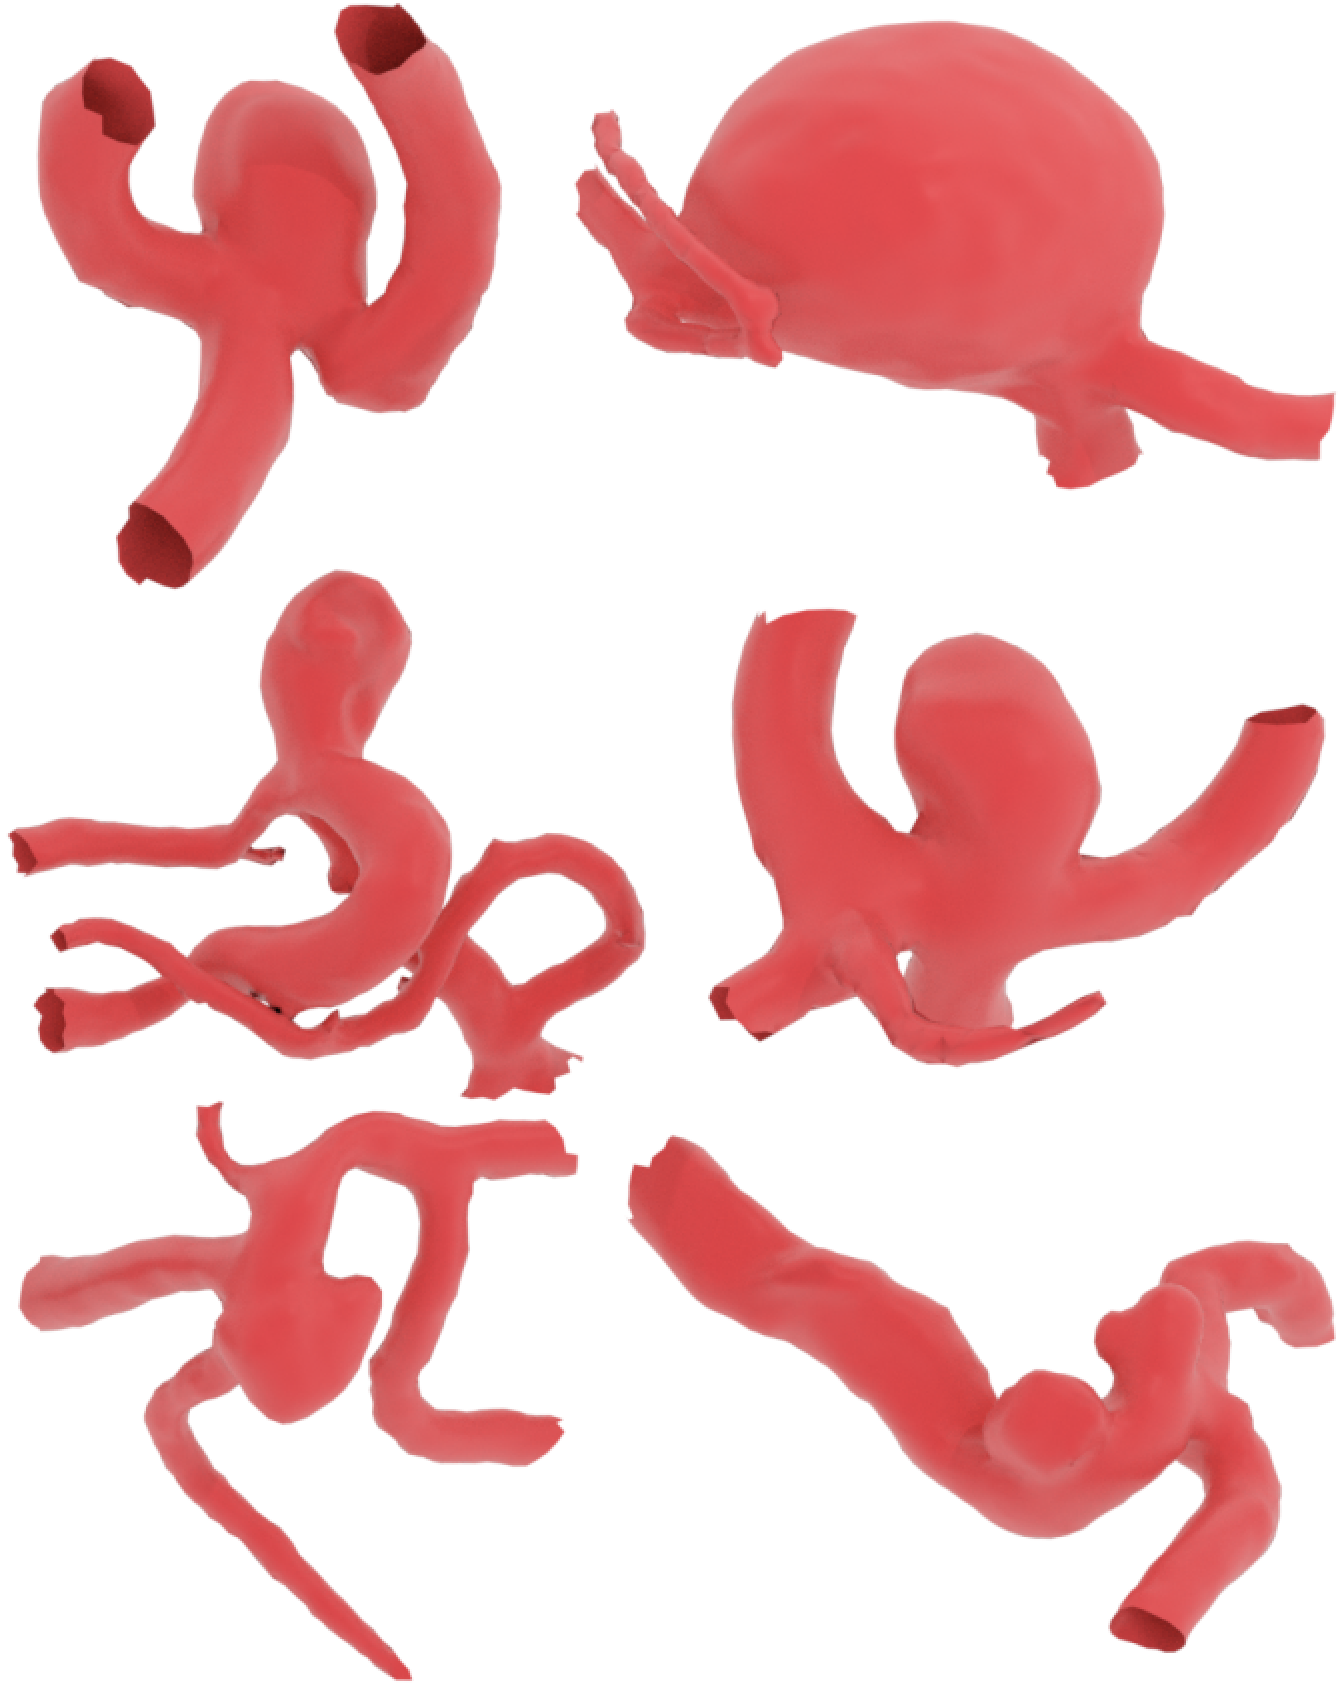
\includegraphics[width=0.5\textwidth]{intra.png}
  \caption{Examples of intracranial aneurysms and vessels from the Intra 3D dataset.}
  \label{fig:intra_aneurysms}
\end{figure}

\begin{figure}[!h]
  \centering
  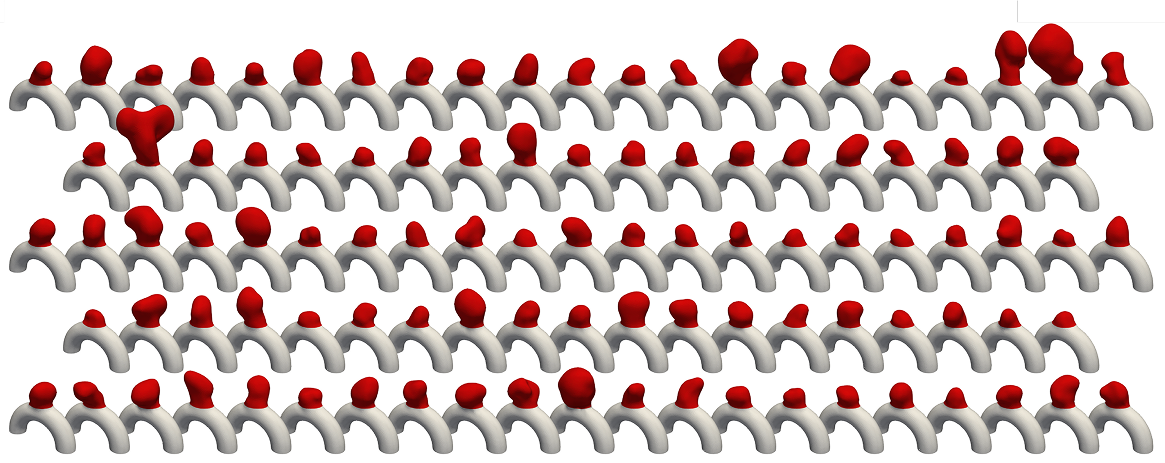
\includegraphics[width=0.5\textwidth]{anxplore.png}
  \caption{Examples of aneurysms from the AnXplore dataset}
  \label{fig:anxplore_aneurysms}
\end{figure}

\section{Related Algorithms} \label{RELATED}

\subsection{TRELLIS encoding}

\begin{figure*}
  \centering
  \begin{subfigure}[b]{0.44\textwidth}
    \centering
    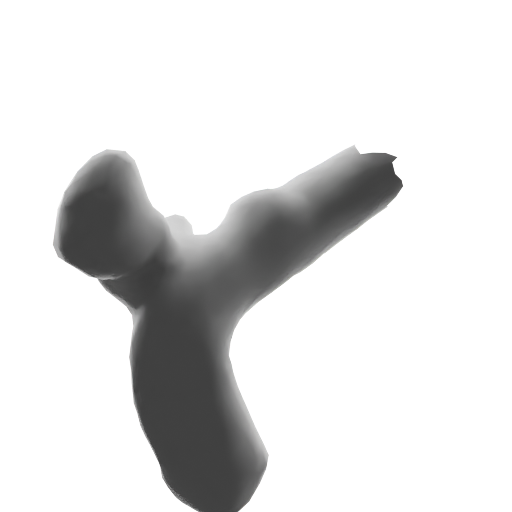
\includegraphics[width=0.22\textwidth]{003.png}
    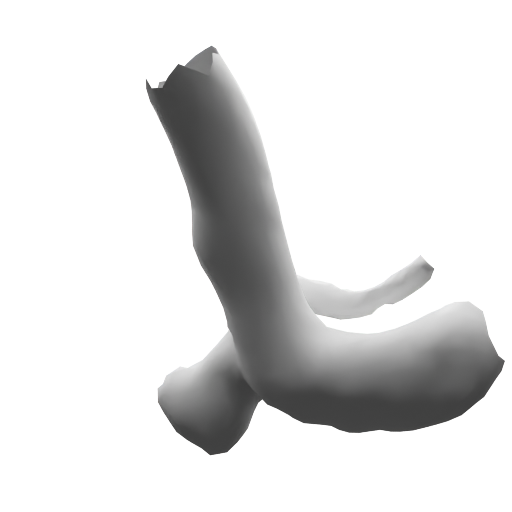
\includegraphics[width=0.22\textwidth]{016.png}
    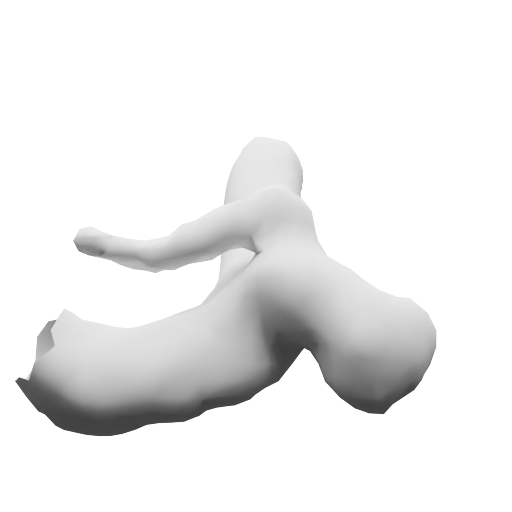
\includegraphics[width=0.22\textwidth]{030.png}
    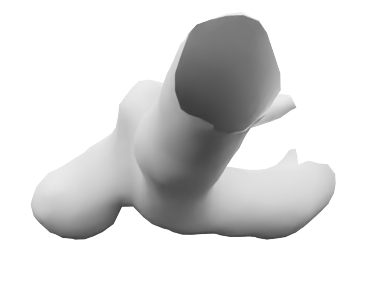
\includegraphics[width=0.22\textwidth]{087.png}
    \vspace{0.2cm} % Add some vertical space between rows
    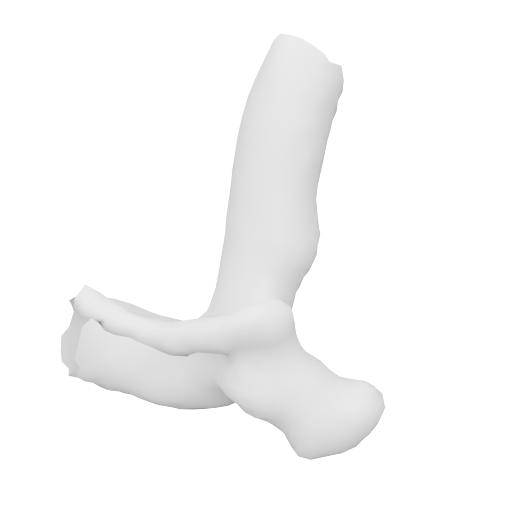
\includegraphics[width=0.22\textwidth]{129.png}
    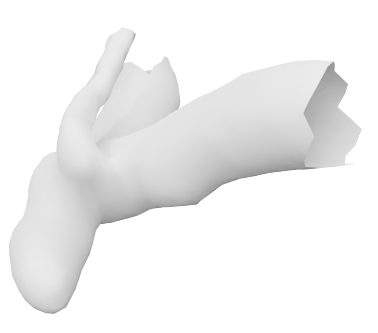
\includegraphics[width=0.22\textwidth]{131.png}
    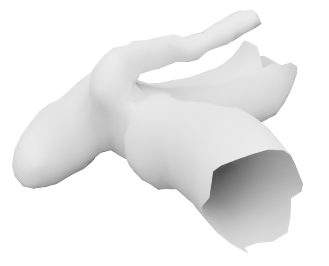
\includegraphics[width=0.22\textwidth]{135.png}
    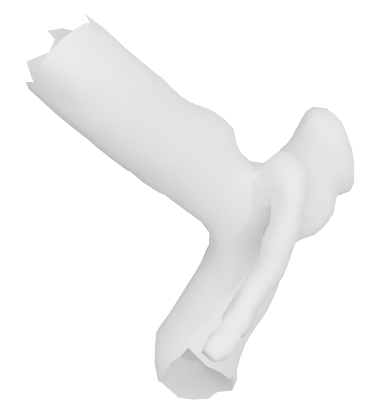
\includegraphics[width=0.22\textwidth]{146.png}
    \caption{Rendered views of 3D objects}
  \end{subfigure}
  \hfill
  \begin{subfigure}[b]{0.44\textwidth}
    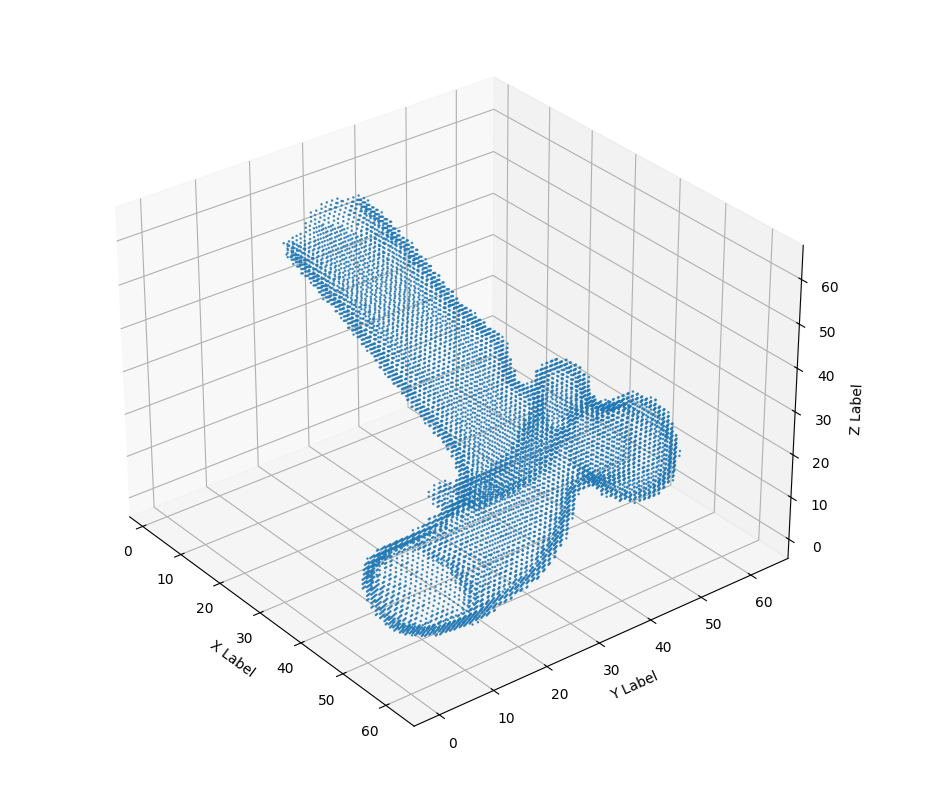
\includegraphics[width=\textwidth]{point_cloud.png}
    \caption{Point cloud}
  \end{subfigure}

  \caption{Illustrations of rendered views and point cloud of an aneurysm from the Intra 3D dataset.}
  \label{fig:combined_views}
\end{figure*}

TRELLIS \citep{xiang2024structured} is an advanced algorithm designed to generate 3D objects from diverse inputs, such as text prompts, multiple 2D views of an object, or another 3D object directly. For the 3D object-to-3D object transformation, TRELLIS employs a robust encoding process to extract detailed features from a mesh, facilitating accurate object reconstruction. This encoding process involves several key steps:

First, the 3D object is rendered from multiple angles to comprehensively capture its geometric details. These rendered views are then voxelized, converting the object into a three-dimensional grid of pixels (voxels) that represent its structure. In our case, this grid is a $64 \times 64 \times 64$ array, where the active voxels correspond to the surface of the object. On average, each object contains approximately 5,000 active voxels.

The voxelized object is then processed to calculate features for each voxel. TRELLIS uses the voxelized representation combined with random views of the object, which are processed using a pre-trained DINOv2 autoencoder \citep{oquab2024dinov2learningrobustvisual}. This autoencoder, based on a vision transformer architecture (ViT) \citep{dosovitskiy2021imageworth16x16words}, extracts high-dimensional features from the rendered images. It is trained to learn robust visual representations, which are then used to encode each voxel in the voxelized grid.

The resulting feature-position pairs are passed into a transformer-based sparse variational autoencoder (VAE). The encoder serializes the inputs with positional encodings and processes them using shifted window attention to efficiently model local interactions. The encoder outputs structured latent tokens, each represented by a 1024-dimensional vector associated with a specific voxel position,

The TRELLIS encoder has already been trained using 500,000 3D assets from 4 public datasets, Objaverse (XL) \citep{deitke2023objaversexluniverse10m3d} , ABO \citep{collins2022abodatasetbenchmarksrealworld}, 3DFUTURE \citep{fu20203dfuture3dfurnitureshape}, and HSSD \citep{khanna2023habitatsyntheticscenesdataset}. We used the encoder directly on Intra 3D \citep{yang2020intra} and AnXplore \citep{anxplore} datasets to extract the features from the meshes of aneurysms and vessels.  

This process is illustrated in Figure \ref{fig:combined_views}.

\subsection{Point Cloud-Based Methods}

Point cloud-based methods are commonly used for 3D object classification and segmentation. We explored two models: PointNet \citep{pointnet} and PointNet++ \citep{pointnetpp}. These two algorithms are effective for processing 3D objects, for example, in the Intra 3D dataset \citep{yang2020intra} or for non-medical data such as ModelNet40 \citep{7298801}.
PointNet is a pioneering architecture that treats a point cloud \( \mathcal{X} = \{x_1, \dots, x_N\} \subset \mathbb{R}^3 \) as an unordered set of points. To maintain permutation invariance, the network applies a shared multi-layer perceptron (MLP) to each point independently and aggregates the resulting features using a symmetric function, typically max pooling:

\vspace{-0.35cm}

\[
g = \max_{i=1,\dots,N} \phi(x_i),
\]

\vspace{-0.1cm}

where \( \phi \) is a shared MLP and \( g \) is a global feature vector summarizing the shape. This global descriptor can be directly used for classification. For segmentation, the global feature is concatenated with local point features before being passed to another shared MLP, enabling point-wise predictions with contextual awareness.

PointNet also includes a learnable alignment module, the T-Net, which estimates an affine transformation to align the input points or features. A regularization term \( \| I - T T^\top \|_F^2 \) is used to ensure that the transformation remains close to orthogonal, enhancing robustness to spatial variations.

\vspace{0.2cm}

PointNet++ builds on PointNet by introducing a hierarchical structure that captures local geometric features at multiple scales. It organizes the input point cloud using a series of \textit{Set Abstraction (SA)} layers, each composed of a sampling step using Farthest Point Sampling (FPS) to select representative points, followed by a grouping step that finds local neighborhoods around each sampled point. Each neighborhood is then processed with a PointNet-like architecture to extract local features.

This process builds progressively more abstract feature representations while preserving spatial locality. To enable dense predictions for tasks like segmentation, PointNet++ uses \textit{Feature Propagation} layers that interpolate features back to the original resolution, leveraging both local and global context through skip connections.

Thanks to its hierarchical design and ability to model non-uniform point densities, PointNet++ substantially outperforms PointNet in complex 3D tasks.


\subsection{Graph Neural Networks (GNNs)}

Graph Neural Networks (GNNs) are a class of neural networks designed to process graph-structured data. They are particularly well-suited for tasks where the data can be represented with nodes and edges, such as 3D meshes.

The main idea behind GNNs is the message-passing mechanism. This mechanism allows nodes in a graph to exchange information with their neighbors. On each iteration or layer, nodes compute messages based on their features and the features of their neighbors. These messages are then aggregated to update the node's representation. This process can be repeated for multiple layers, allowing nodes to gather information from increasingly distant neighbors.

This concept has been adapted for 3D aneurysm modeling to simulate hemodynamics in \citep{graphphysics}. The encode-process-decode framework facilitates the application of GNNs on mesh structures, enabling the simulation of blood flow in aneurysms. Simulation performance is further enhanced by attention mechanisms \citep{VaswaniSPUJGKP17}, which focus computation on the most relevant mesh regions, thereby increasing both accuracy and efficiency.

For the simulation, \citep{graphphysics} represents the mesh by an undirected graph \( G = (V, E) \) with nodes \( V = \{x_i\}_{i=1}^N \), each \( x_i \in \mathbb{R}^p \). The input is the matrix \( X \in \mathbb{R}^{N \times p} \). The model follows an encode-process-decode architecture: the encoder maps \( X \) into a latent space \( Z_0 = \text{MLP}(X) \in \mathbb{R}^{N \times d} \) using two linear layers. The processor applies \( L \) transformer blocks; each block uses masked multi-head self-attention with the adjacency matrix \( A \in \{0,1\}^{N \times N} \) as a mask, computed as
\[
\text{Attention}(Z) = \text{softmax}\left(\frac{QK^\top \odot A}{\sqrt{d}}\right)V,
\]
where \( Q, K, V \) are learned linear projections of \( Z \). A Gated MLP with Gaussian Error Linear Unit (GeLU) \citep{hendrycks2023gaussianerrorlinearunits} non-linearity follows, defined as
\[
Z = W_f \big( \text{GeLU}(W_l Z + b_l) \odot (W_r Z + b_r) \big) + b_f,
\]
With residual connections and RMS (Root Mean Square)  normalization \citep{zhang2019rootmeansquarelayer} after each sub-layer. The decoder maps \( Z_L \) back to the output space via two linear layers.

To enhance the receptive field and information flow, the adjacency matrix is augmented by dilated adjacency with \( k \)-hop neighbors, random edges added dynamically, and global attention connecting important nodes to all others.


\section{Datasets} \label{DATASET}

\subsection{Intra 3D Dataset} \label{INTRA3D}

The Intra 3D dataset \citep{yang2020intra} contains 3D models of intracranial aneurysms and healthy blood vessels, reconstructed from 2D MRA scans, used for classification and segmentation tasks. The classification dataset is imbalanced, containing 1,694 healthy vessels and 215 aneurysms. There are also 116 annotated aneurysms used to train segmentation models, which can also be used to supplement the classification dataset. The original paper also presents classification and segmentation results using models such as PointNet \citep{pointnet}, PointNet++ \citep{pointnetpp}, PointCNN \citep{pointcnn}, SO-net \citep{sonet}, and PointConv \citep{pointconv}.

In our study, we used the meshes provided by the dataset and processed them as 3D objects to extract the surface features using TRELLIS \citep{xiang2024structured}. We encoded all the aneurysms from both the classification and segmentation datasets, but only 1,150 out of the 1,694 vessels from the classification dataset. This resulted in 331 aneurysms and 1150 vessels, represented as point clouds with positions and 1024-dimensional features. Those point clouds were sampled to obtain a fixed number of points per object, which is necessary for the neural networks we used. We did three different samplings: 512, 1024, and 2048 points per object, following the approach in Intra 3D \citep{yang2020intra}. 

\subsection{AnXplore Dataset} \label{ANXPLORE}

The AnXplore dataset \citep{anxplore} contains 101 3D models of intracranial aneurysms, each with associated blood flow simulations, in the form of volumetric data. These aneurysms are extracted from the 116 annotated aneurysms in Intra3D \citep{yang2020intra}. To generate each model, the head of each aneurysm was isolated and placed on the same uniform vessel, meaning all aneurysms in AnXplore \citep{anxplore} are located on the same vessel but vary in shape and size. For TRELLIS \citep{xiang2024structured}, we extract the surface mesh from the first time step of each simulation, as the external aneurysm geometry does not change during the simulation.

\section{Analysis of the TRELLIS features} \label{FEATURES}

We conducted several analyses on the TRELLIS features to better understand them and to evaluate how well these features represent the objects.

First, for each object, we computed various statistical metrics. Since each point is described by an 1024-dimensional feature vector, we calculated the mean, standard deviation, minimum, and maximum for each feature across all points in an object. Thus, each object is represented by four vectors of size 1024. We then performed 2D PCA on these vectors for each category, first on the Intra3D dataset \citep{yang2020intra}, and then on the combined Intra3D and AnXplore datasets \citep{anxplore}. The goal of the combined analysis was to assess whether the AnXplore aneurysms are encoded differently compared to the Intra3D aneurysms. Results for the mean and standard deviation features are shown in Figure \ref{fig:pca}; additional results are provided in the appendix.

To investigate whether other components could provide a clearer separation of aneurysms, we also performed t-SNE on the combined dataset, as shown in Figure \ref{fig:tsne} for the mean features.

\begin{figure}[h]
  \centering
  \begin{flushleft}
    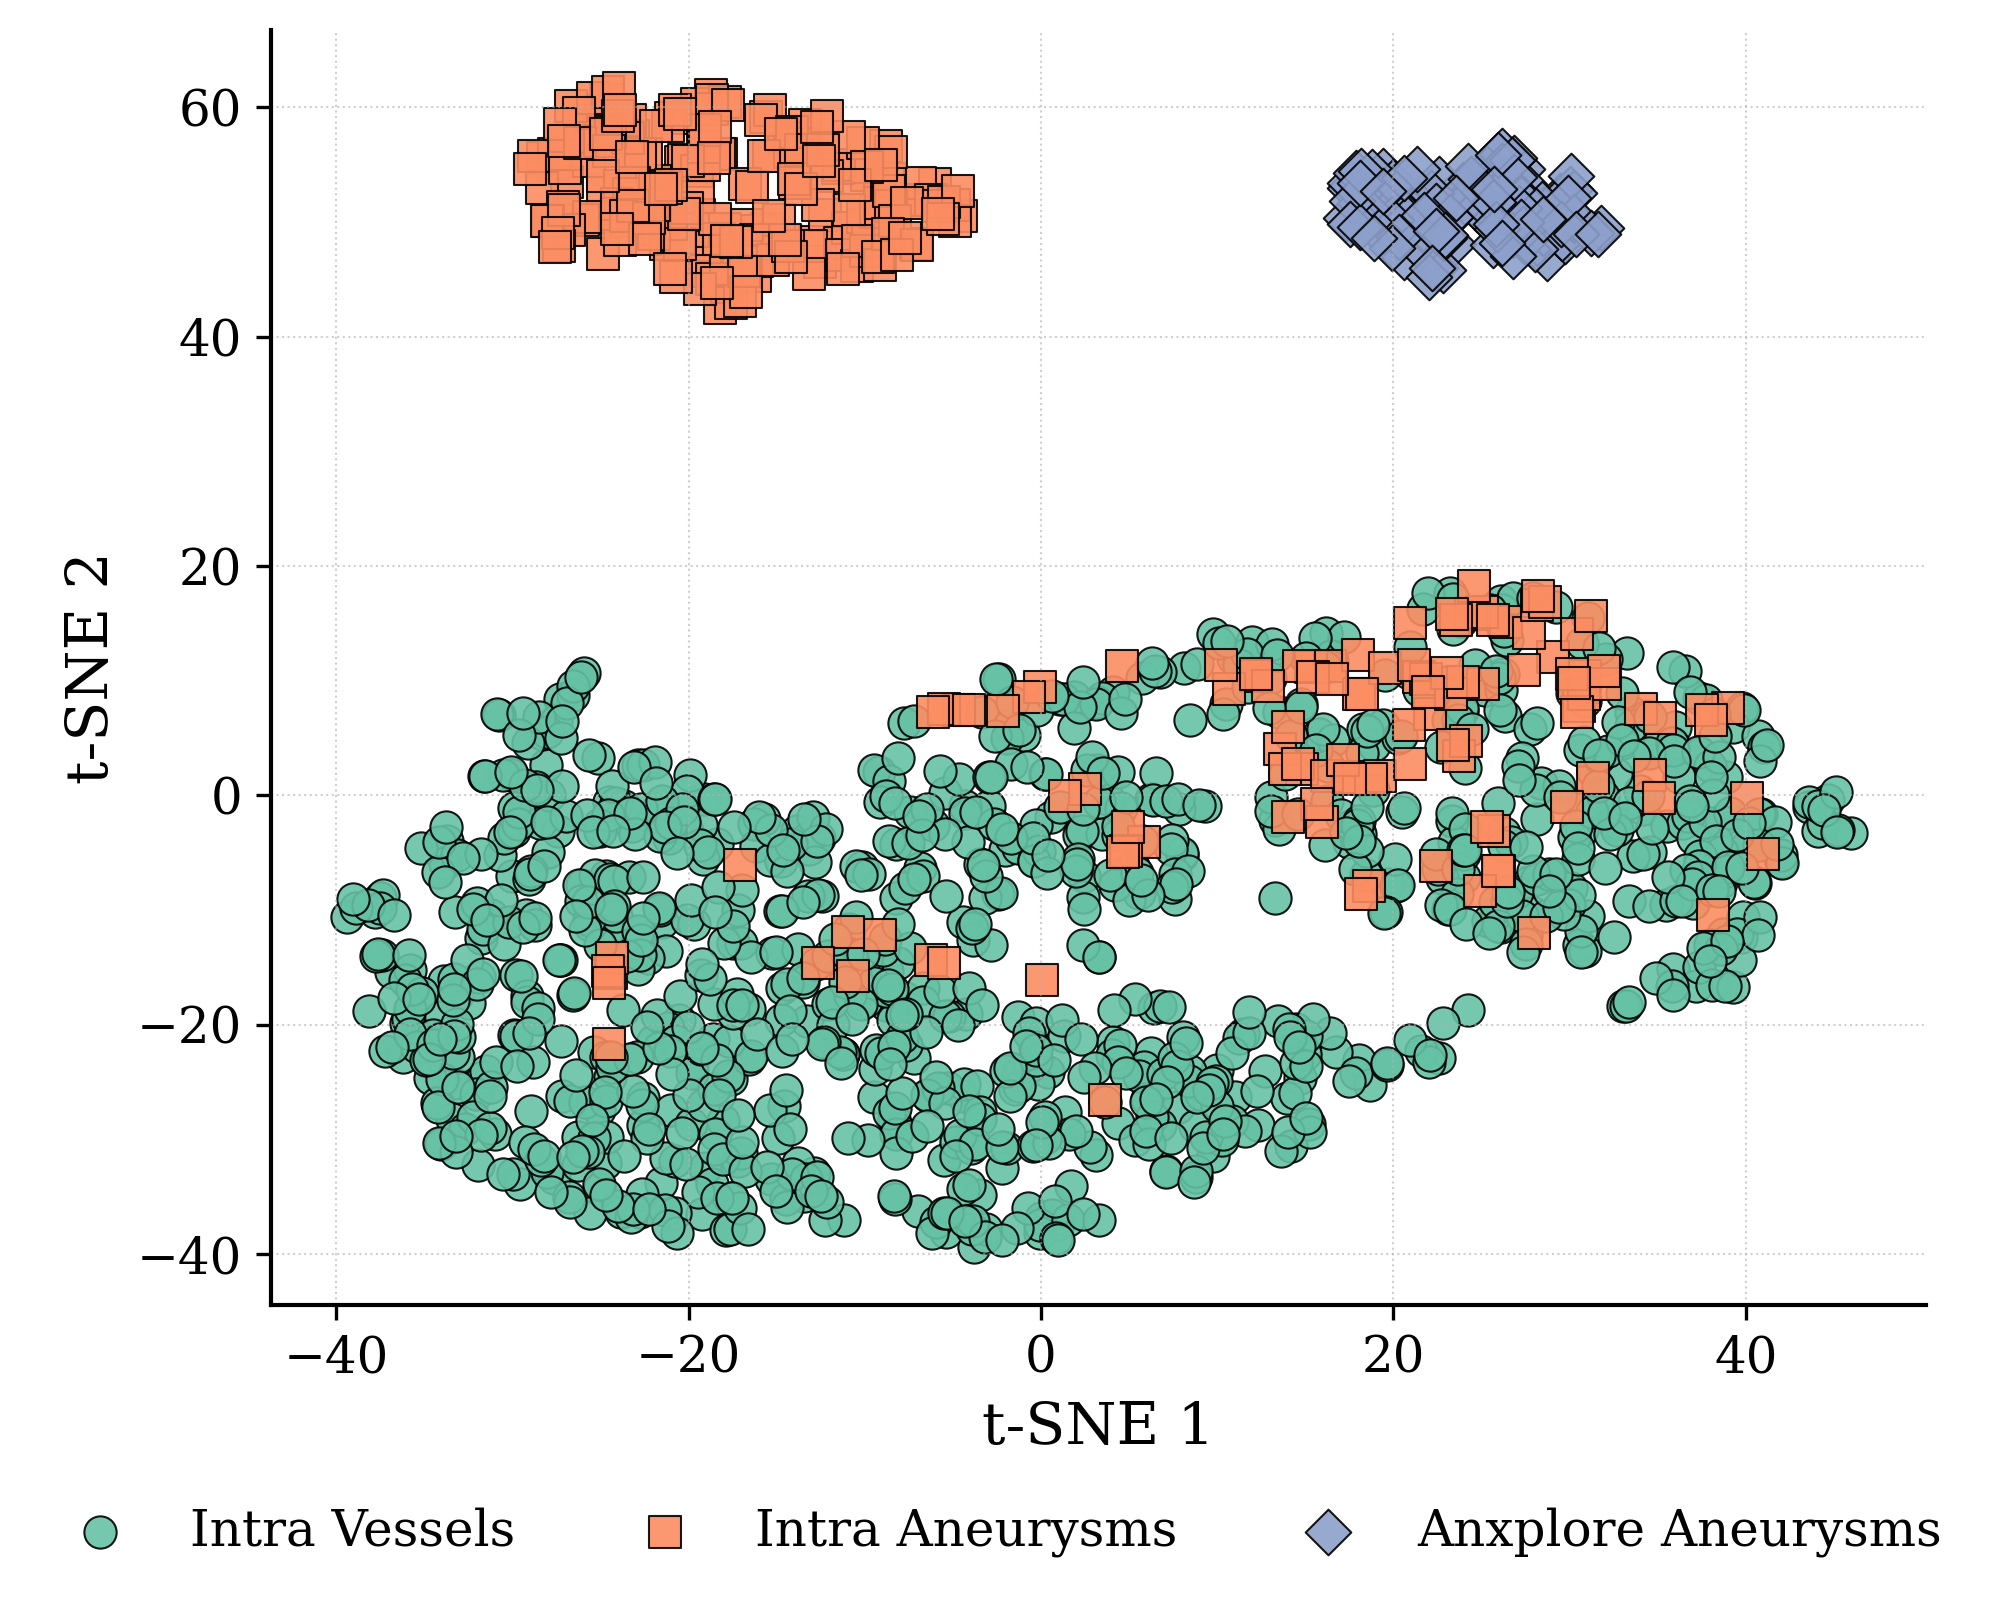
\includegraphics[width=0.47\textwidth]{t-sne_mean.png}
  \end{flushleft}  
  \caption{Result of t-SNE on the mean features of the Intra3D dataset for classification and AnXplore dataset.}
  \label{fig:tsne}
\end{figure}

For the Intra3D dataset alone, we observe that the mean and standard deviation features effectively separate aneurysms and vessels, while the minimum and maximum features do not provide a clear separation. 

When combining with the AnXplore dataset, we observe that the two datasets are separated for three out of the four metrics. This suggests that the characteristics of the vessel on which an aneurysm is located have a strong influence on the extracted features. Nevertheless, aneurysms from AnXplore are often located in the same region of PCA space as aneurysms from Intra3D. With t-SNE, the separation becomes even more pronounced: AnXplore is consistently well-separated from Intra3D, and within Intra3D, aneurysms and vessels are distinctly separated using the mean and minimum features.

To further assess the utility of PCA and the extracted features for classification, we trained machine learning algorithms on the resulting 2D projections from the Intra3D dataset, as discussed in the following section.

\begin{figure*}
  \centering
  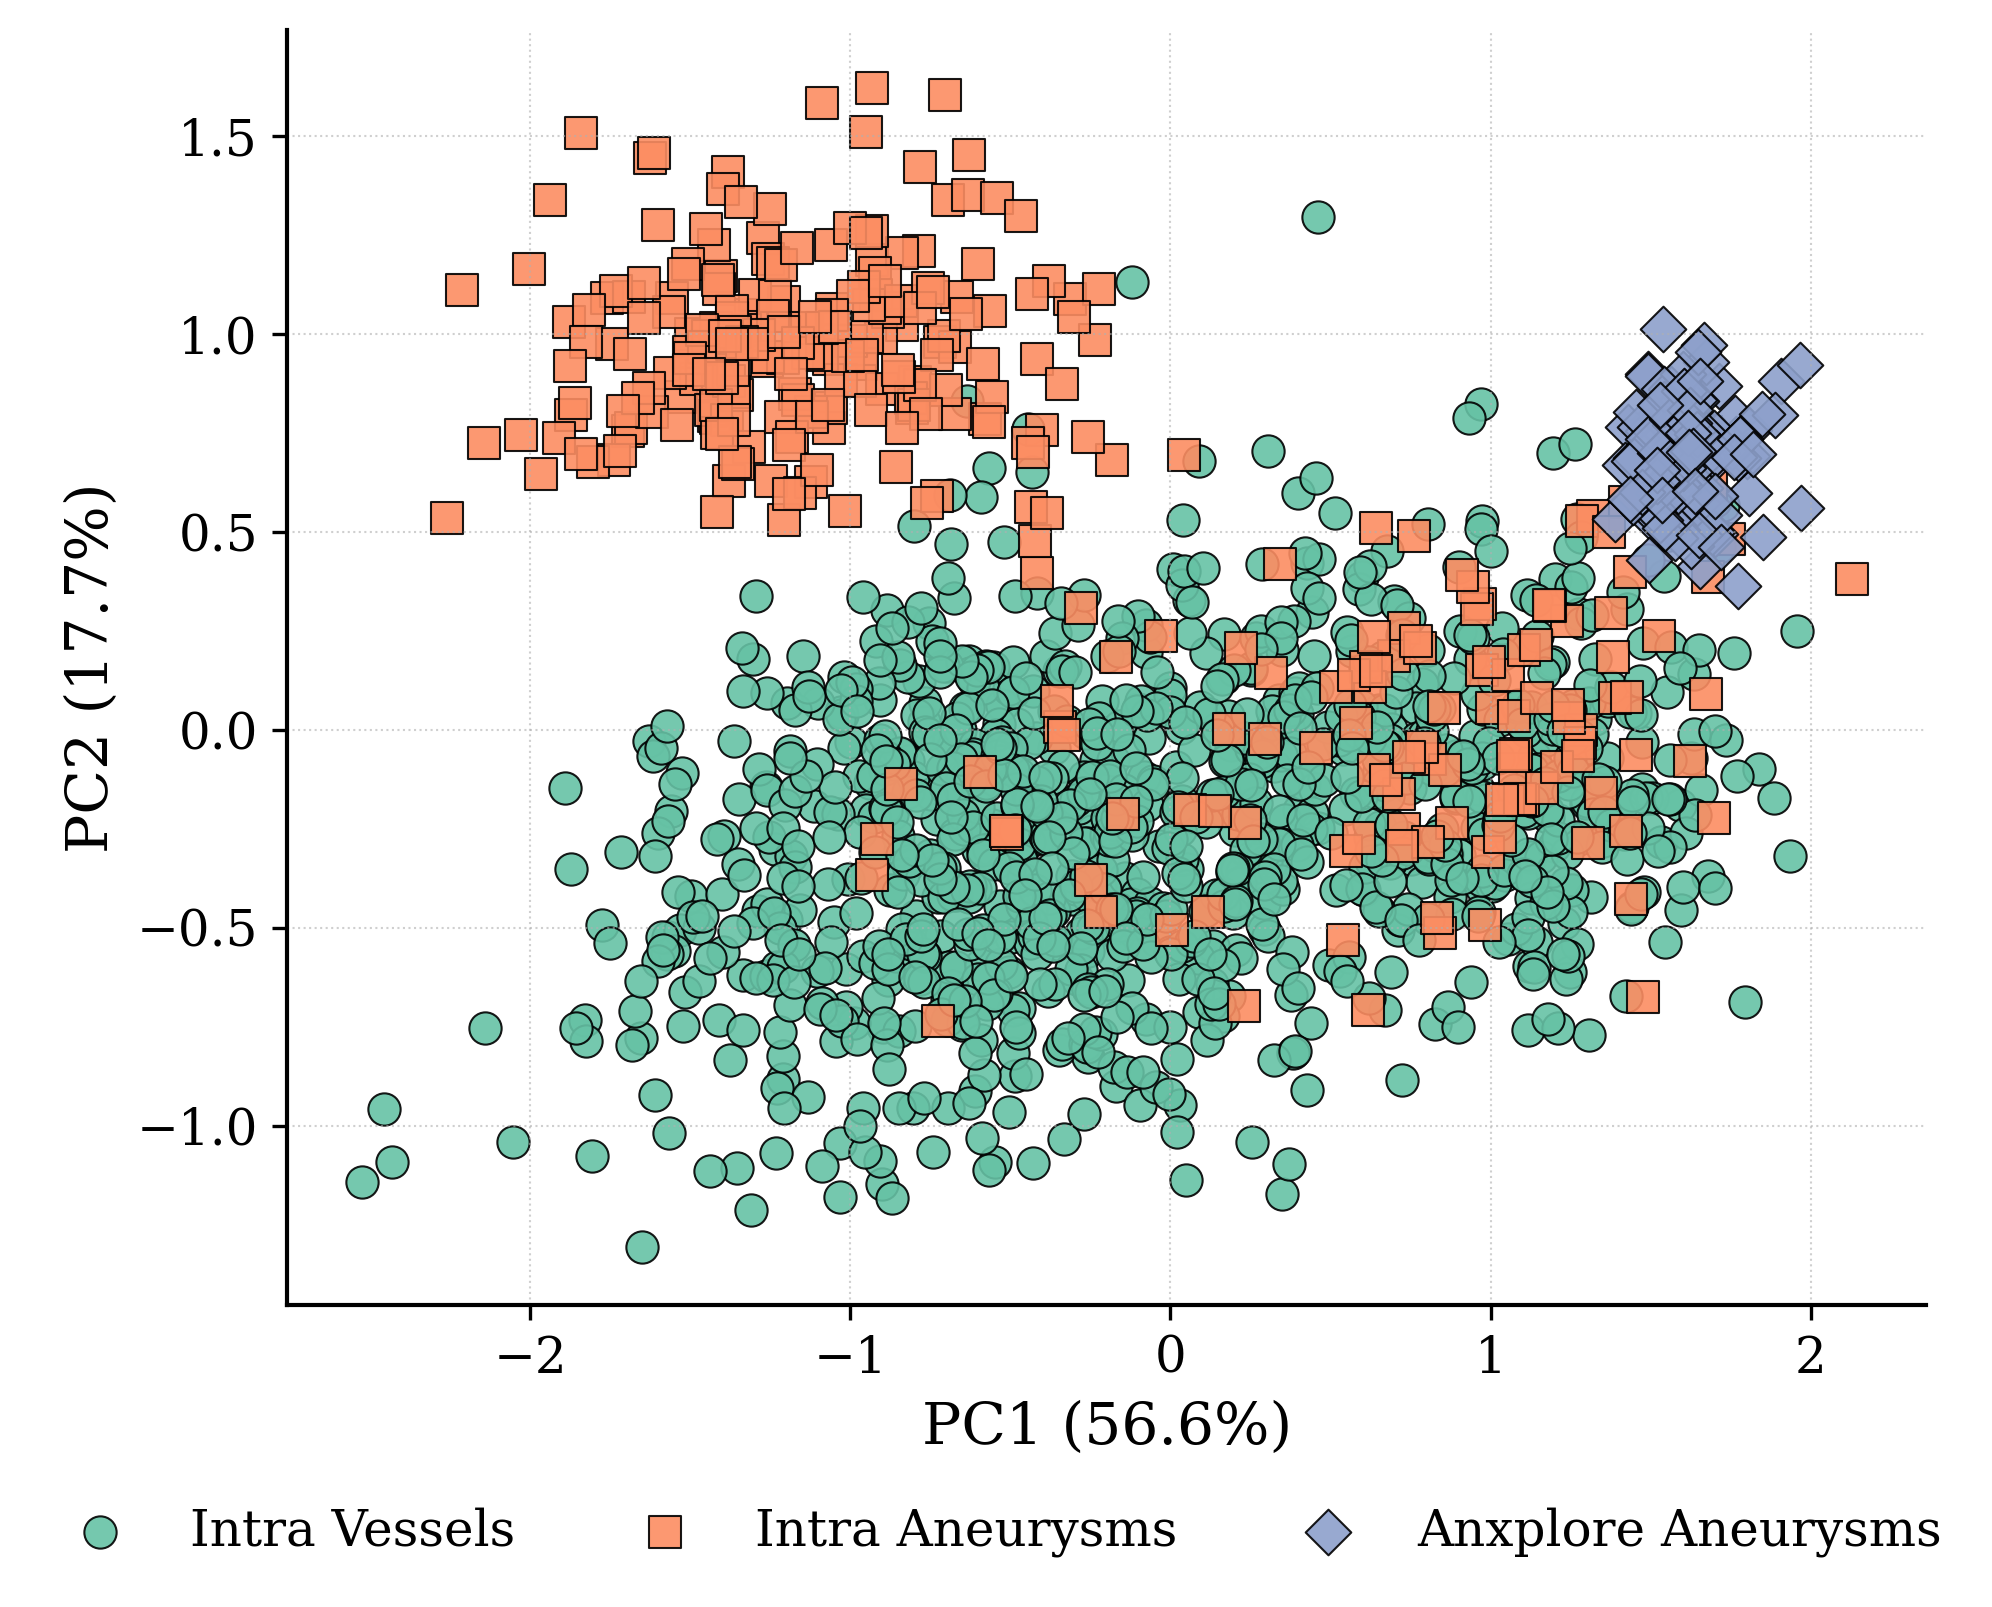
\includegraphics[width=0.32\textwidth]{pca_mean.png}
  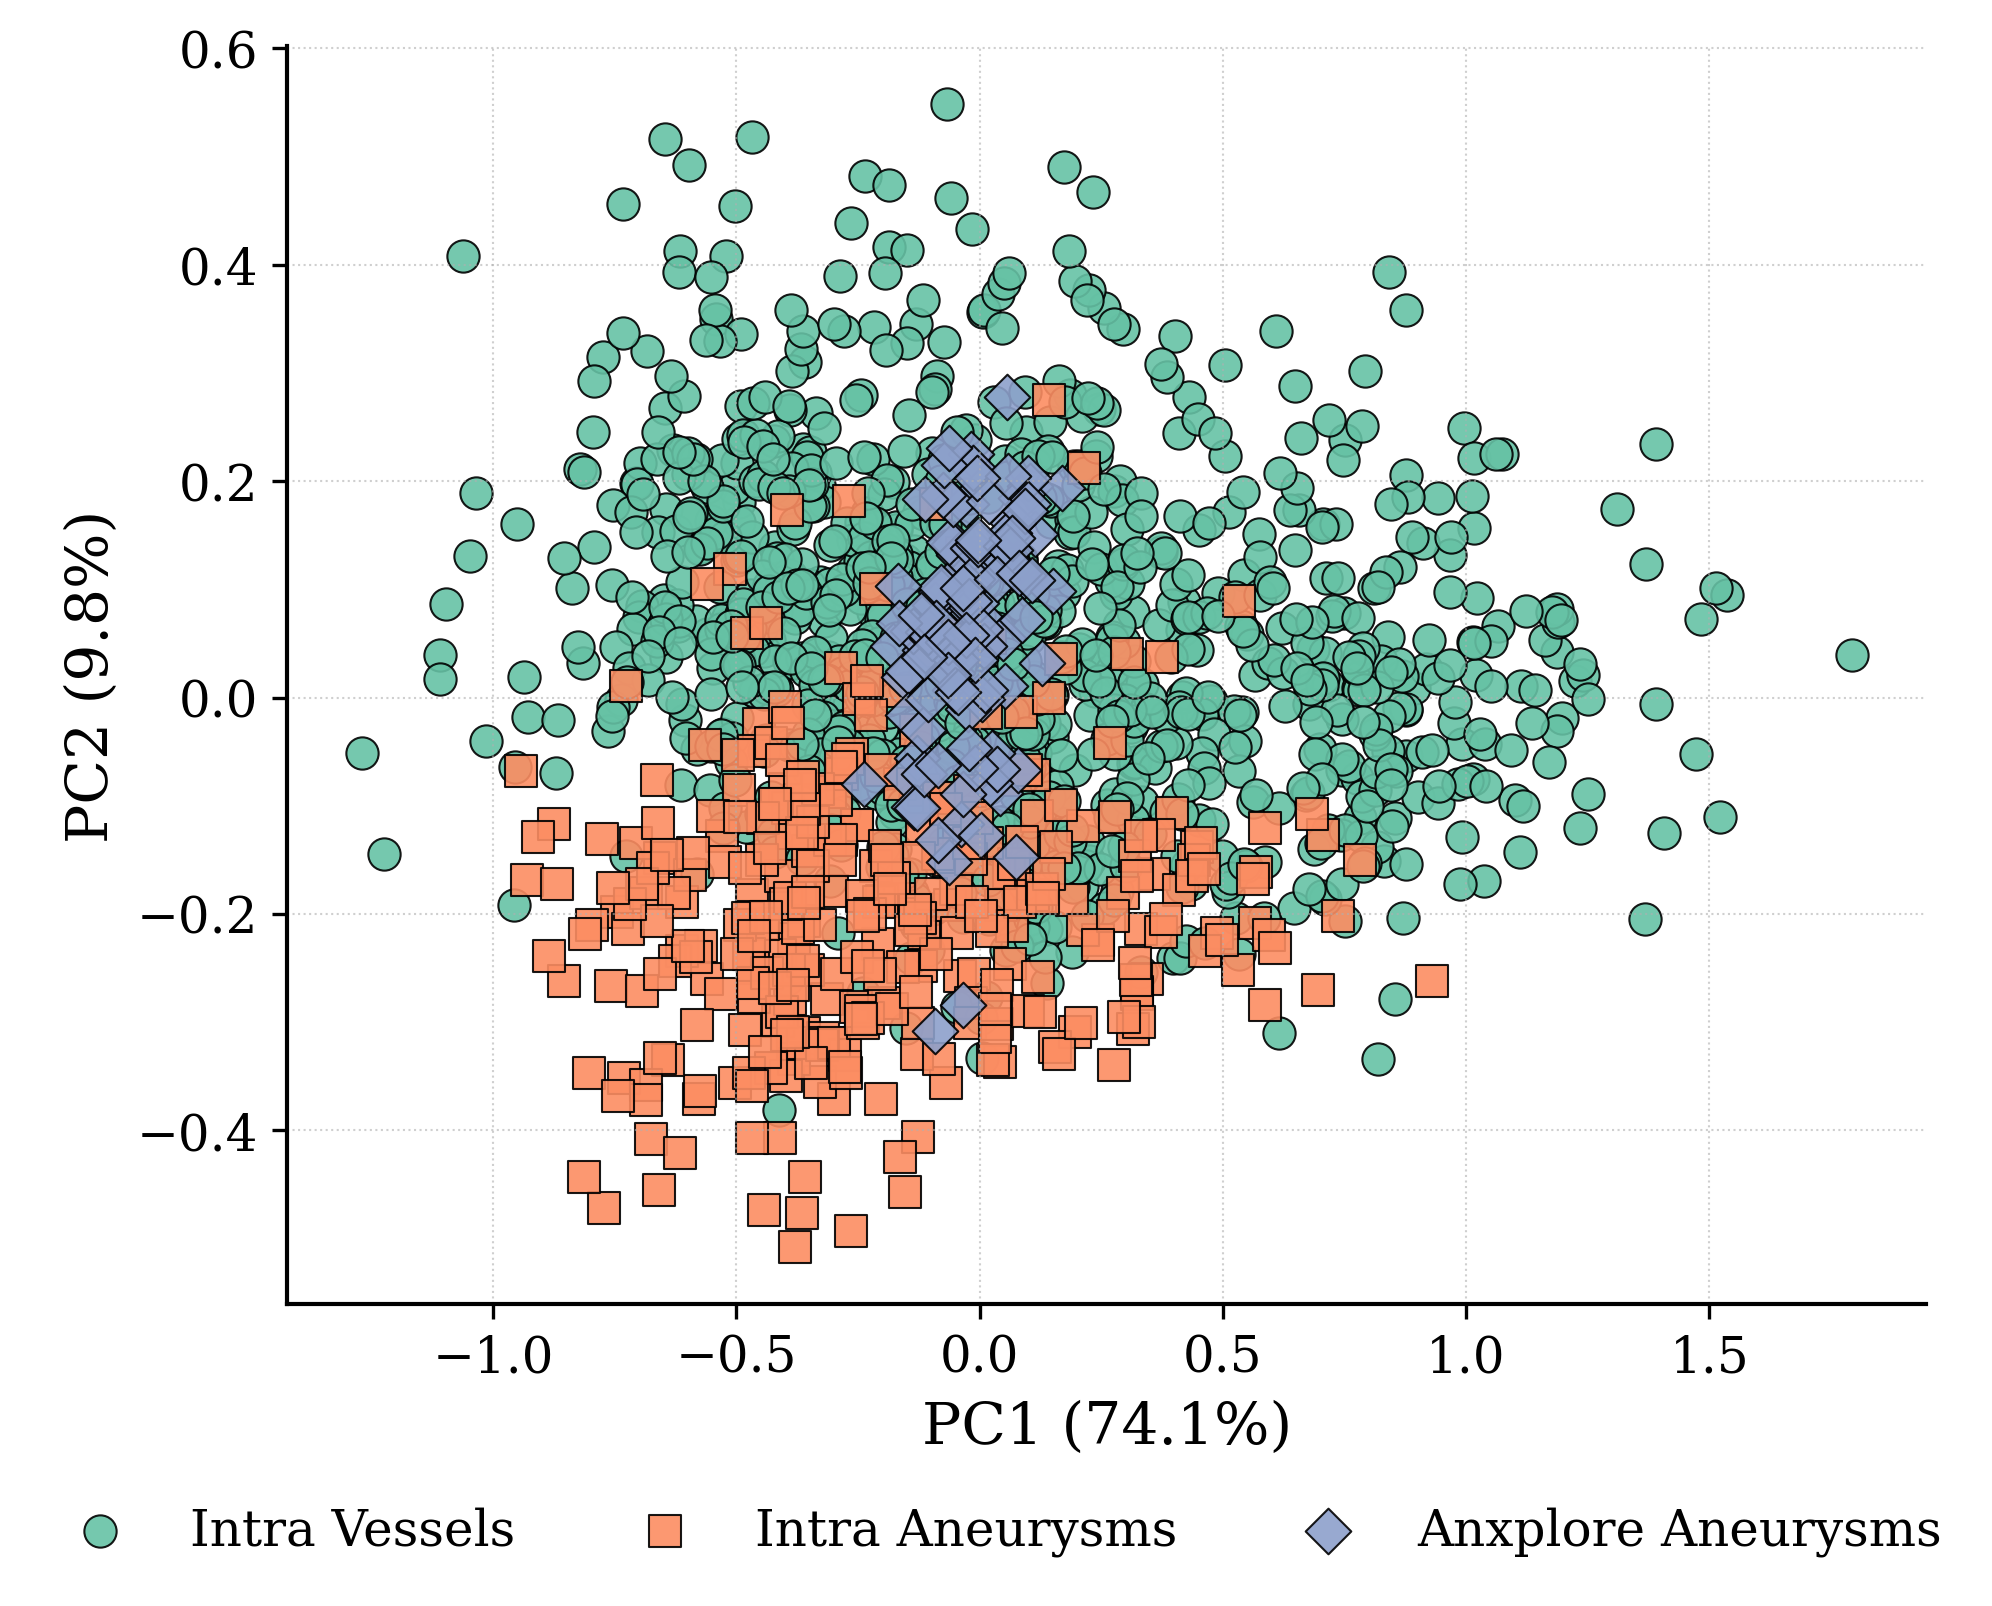
\includegraphics[width=0.32\textwidth]{pca_std.png}
  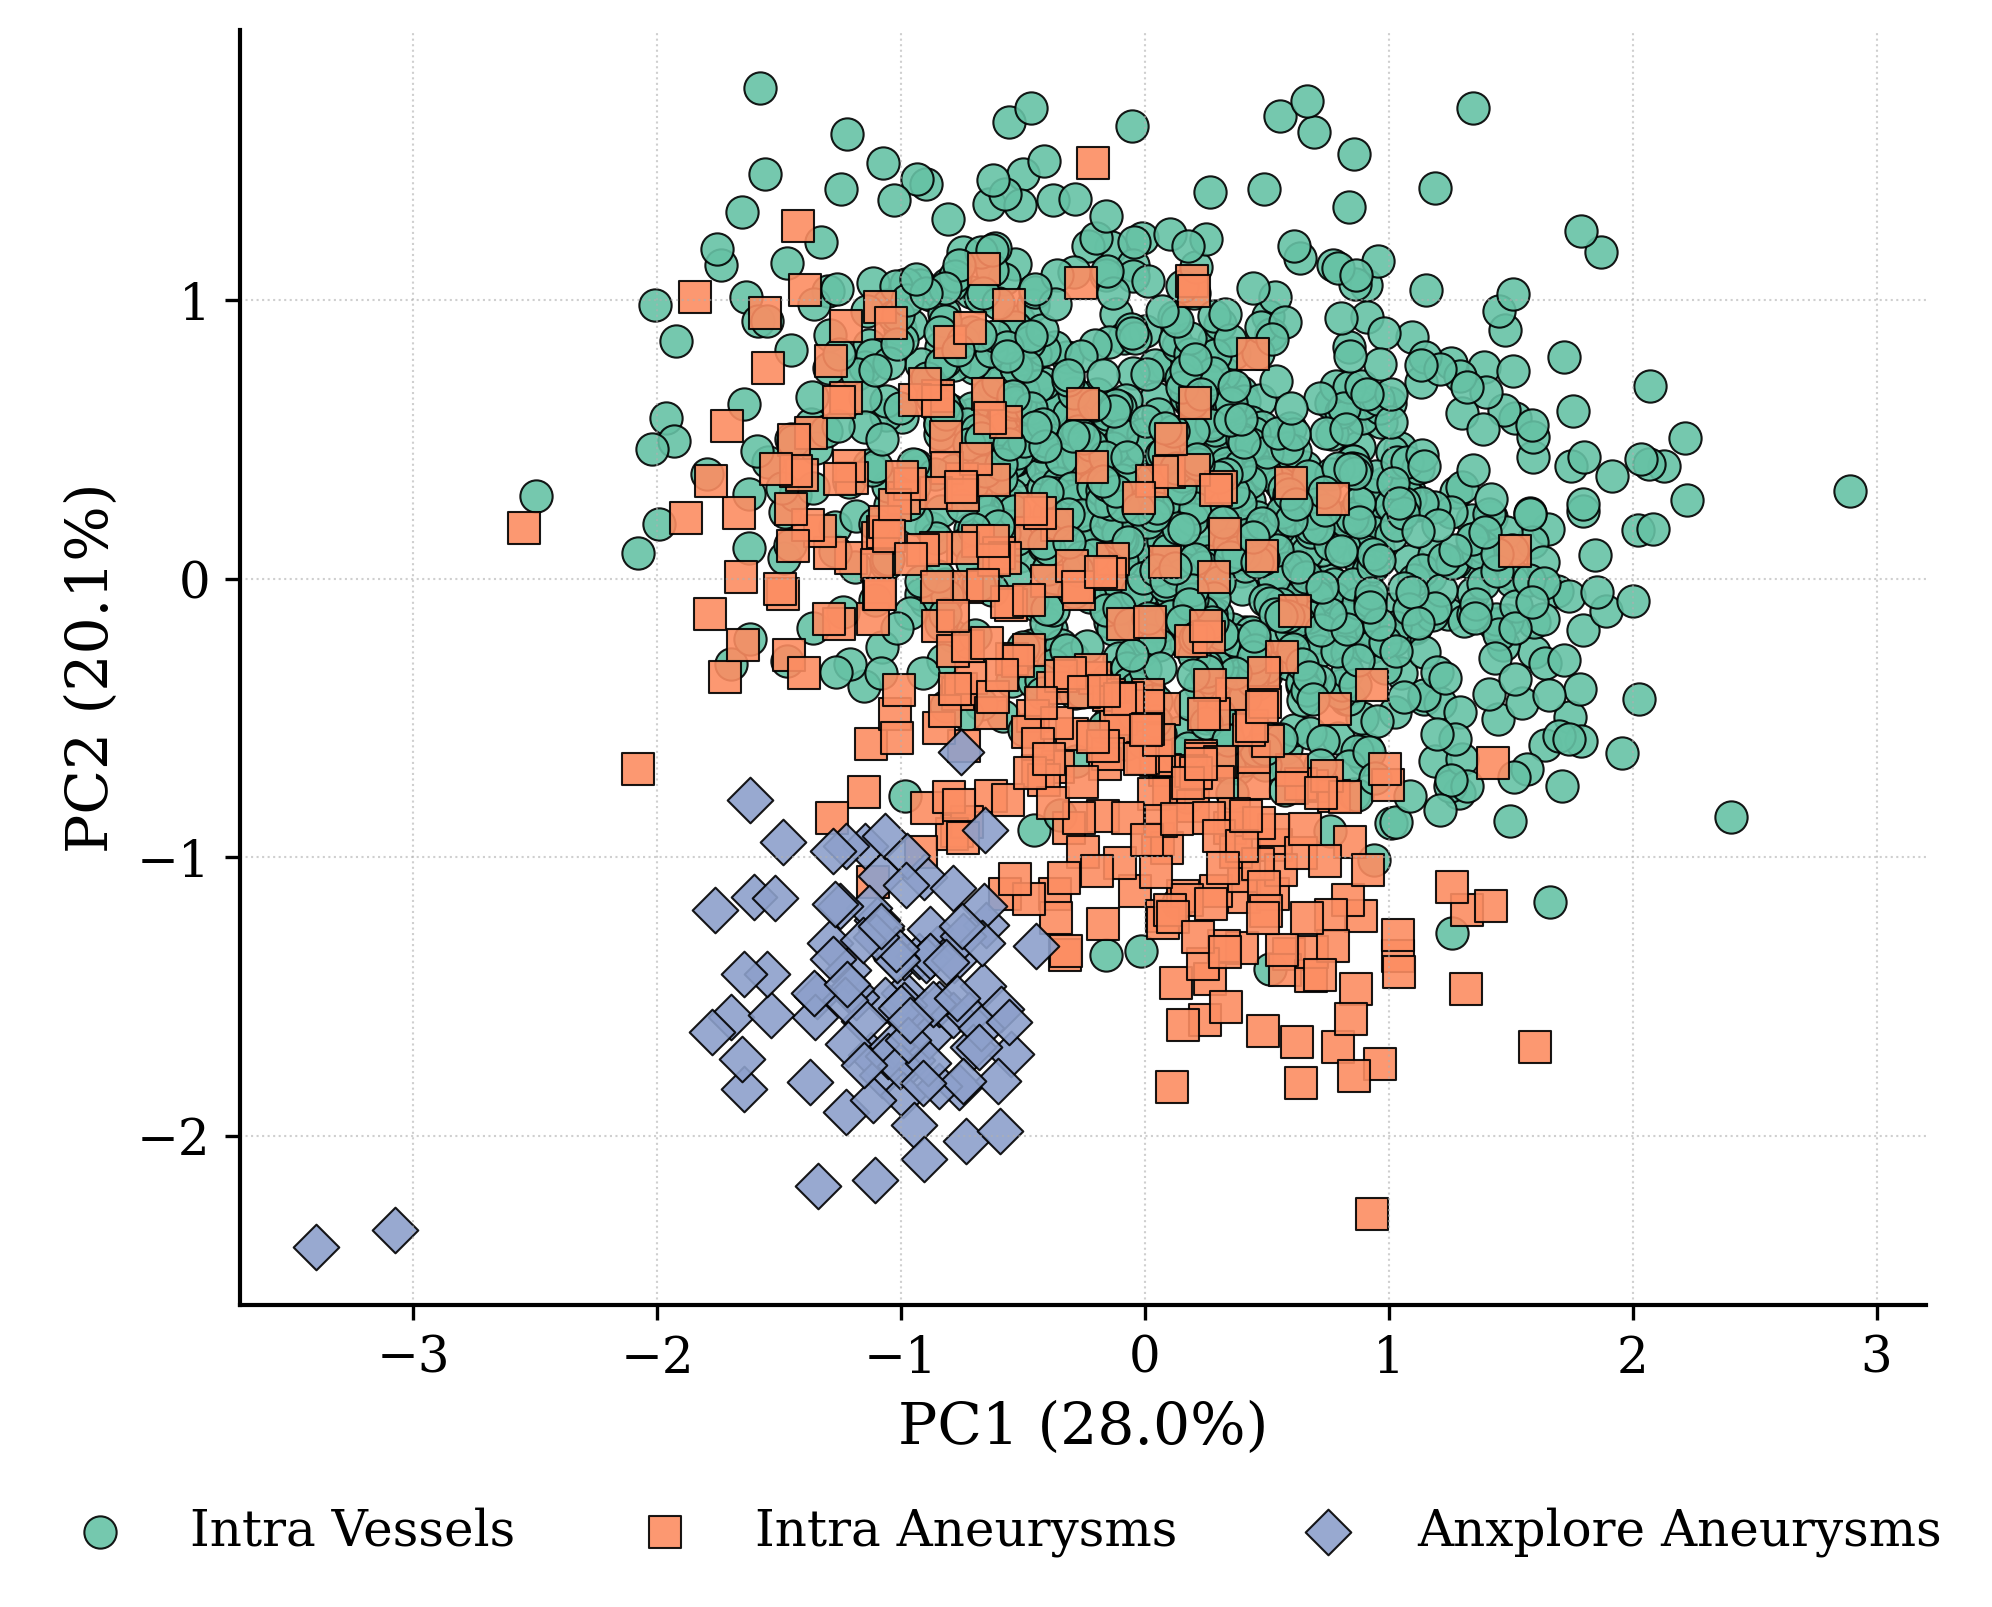
\includegraphics[width=0.32\textwidth]{pca_min.png}
  \caption{Results of PCA on the Intra3D and AnXplore datasets. The left figure shows the mean features, the middle figure shows the standard deviation features, and the right figure shows the minimum features.}
  \label{fig:pca}
\end{figure*}


We compute the mean, standard deviation, minimum, and maximum features for points from the aneurysm and vessel parts separately and perform t-SNE over the 116 annotated aneurysms. This proved to be highly effective and revealed that the two parts, the aneurysm and the vessel, are encoded distinctly. Results are shown in Figure~\ref{fig:aneu_seg}. To further study these differences, we also performed 2D PCA and t-SNE on all the features from a single element, which yielded a clear separation between the aneurysm and vessel parts. This indicates that the features extracted by TRELLIS \citep{xiang2024structured} are effective for distinguishing between these two components of the 3D model. Results are shown in Figure \ref{fig:aneu_seg_2}. All the figures can be found in the appendix.


\begin{figure}[h!]
  \centering
  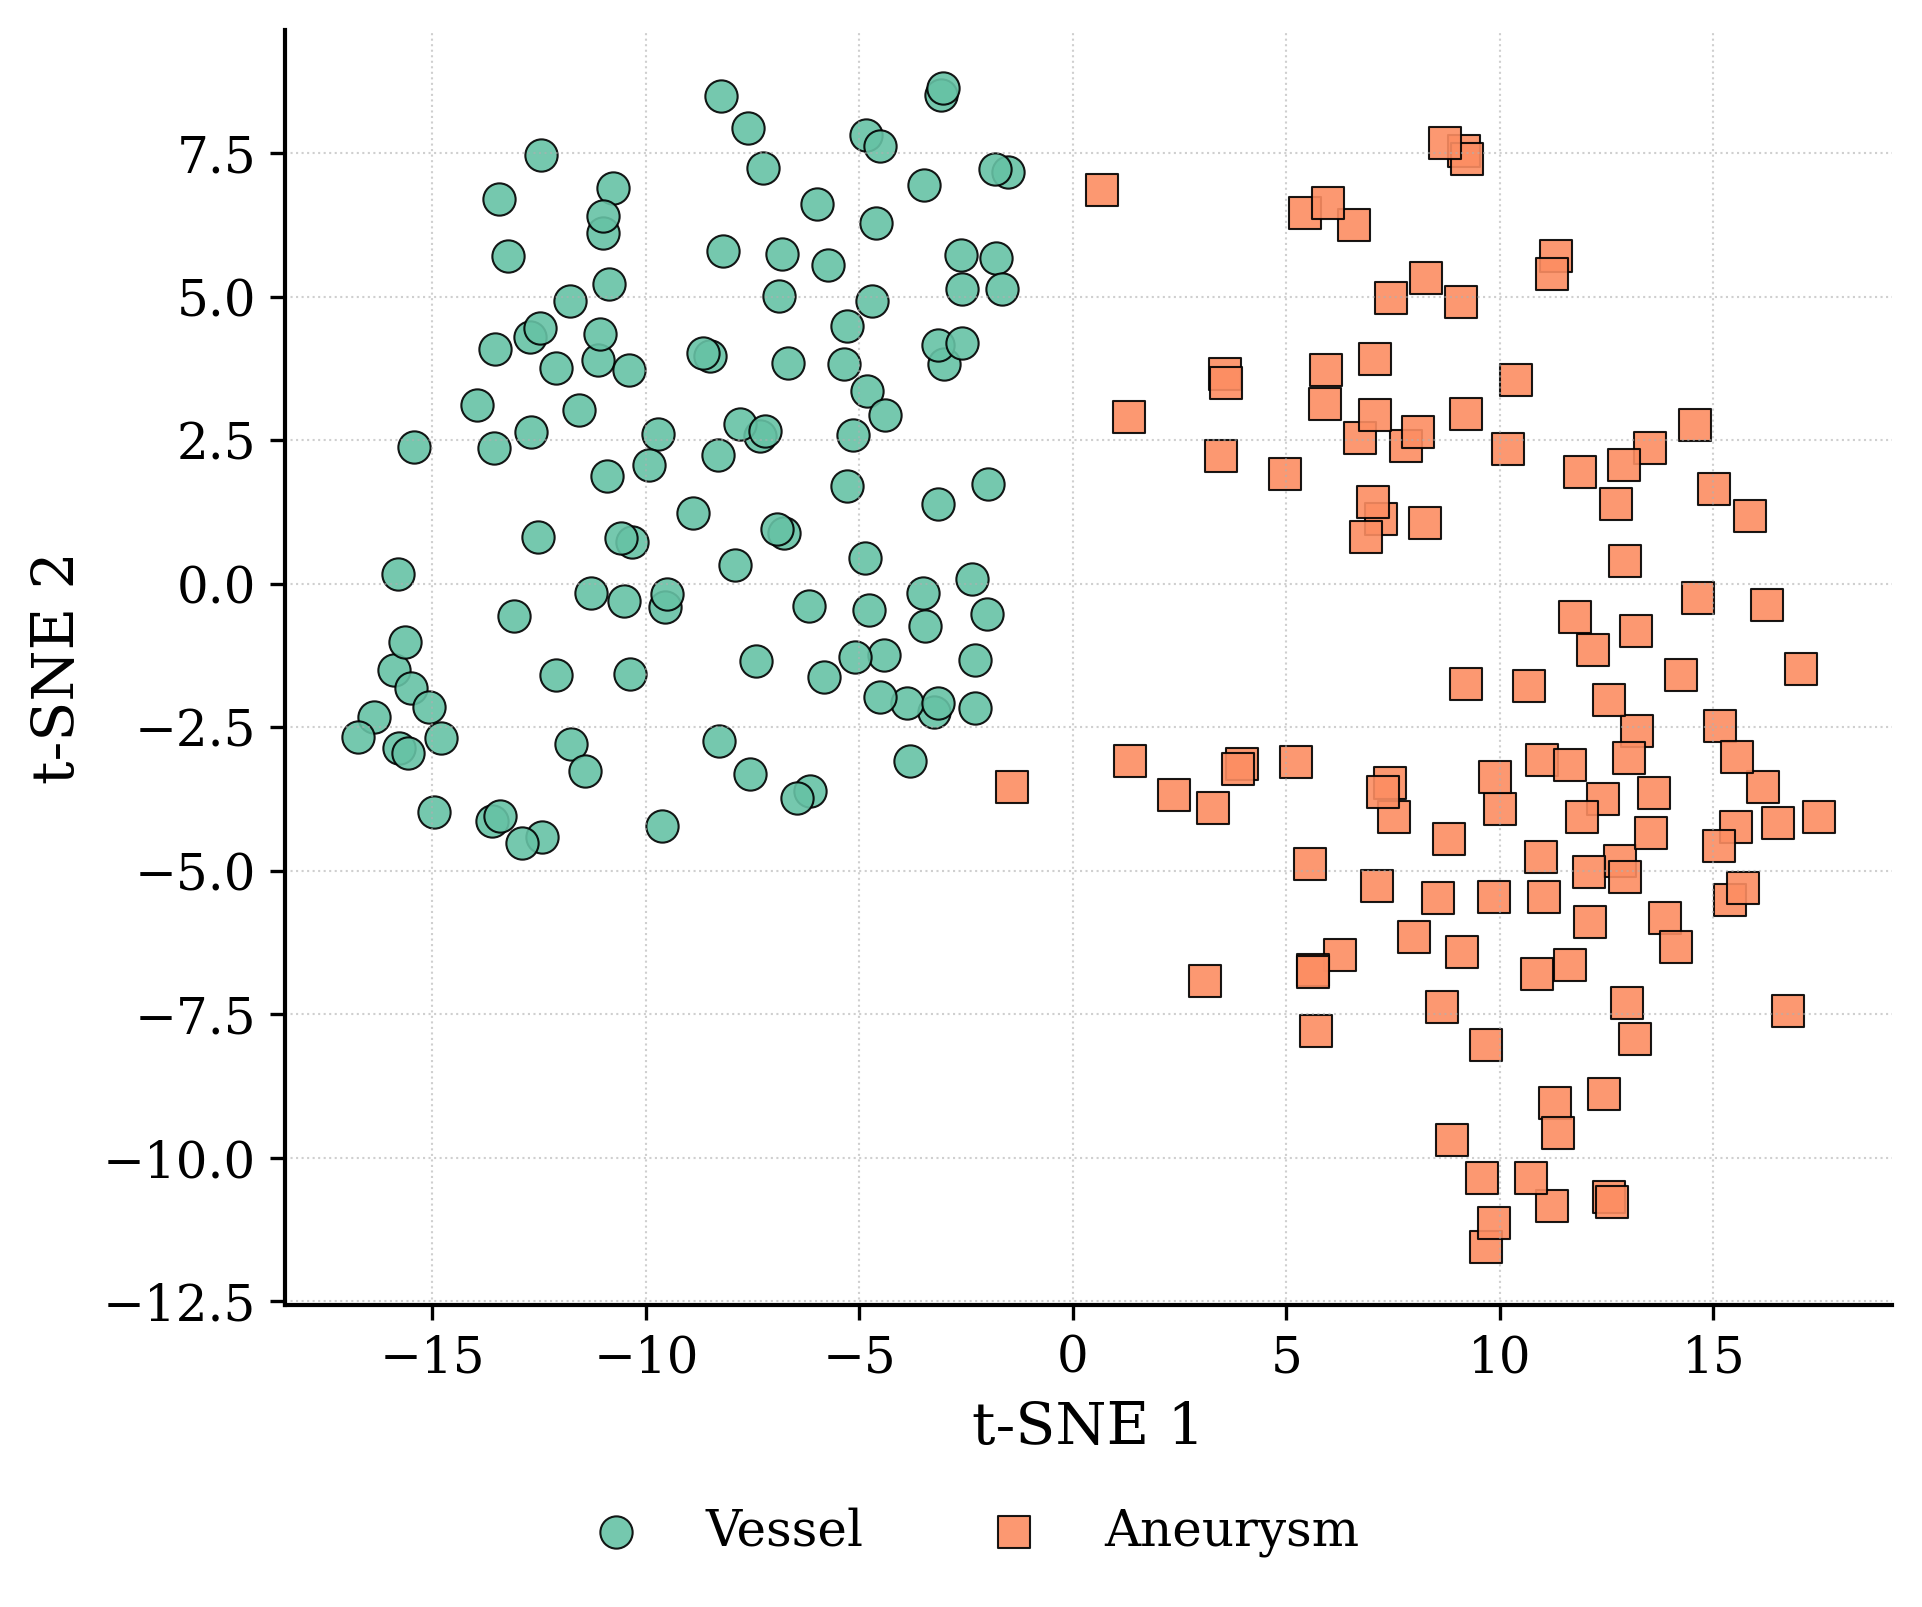
\includegraphics[width=0.47\textwidth]{t-sne_global_mean.png}
  \caption{Results of t-SNE on annotated aneurysms from Intra3D \citep{yang2020intra} using the mean features of the aneurysm and vessel parts.}
  \label{fig:aneu_seg}
\end{figure}

\begin{figure}[h!]
  \centering
  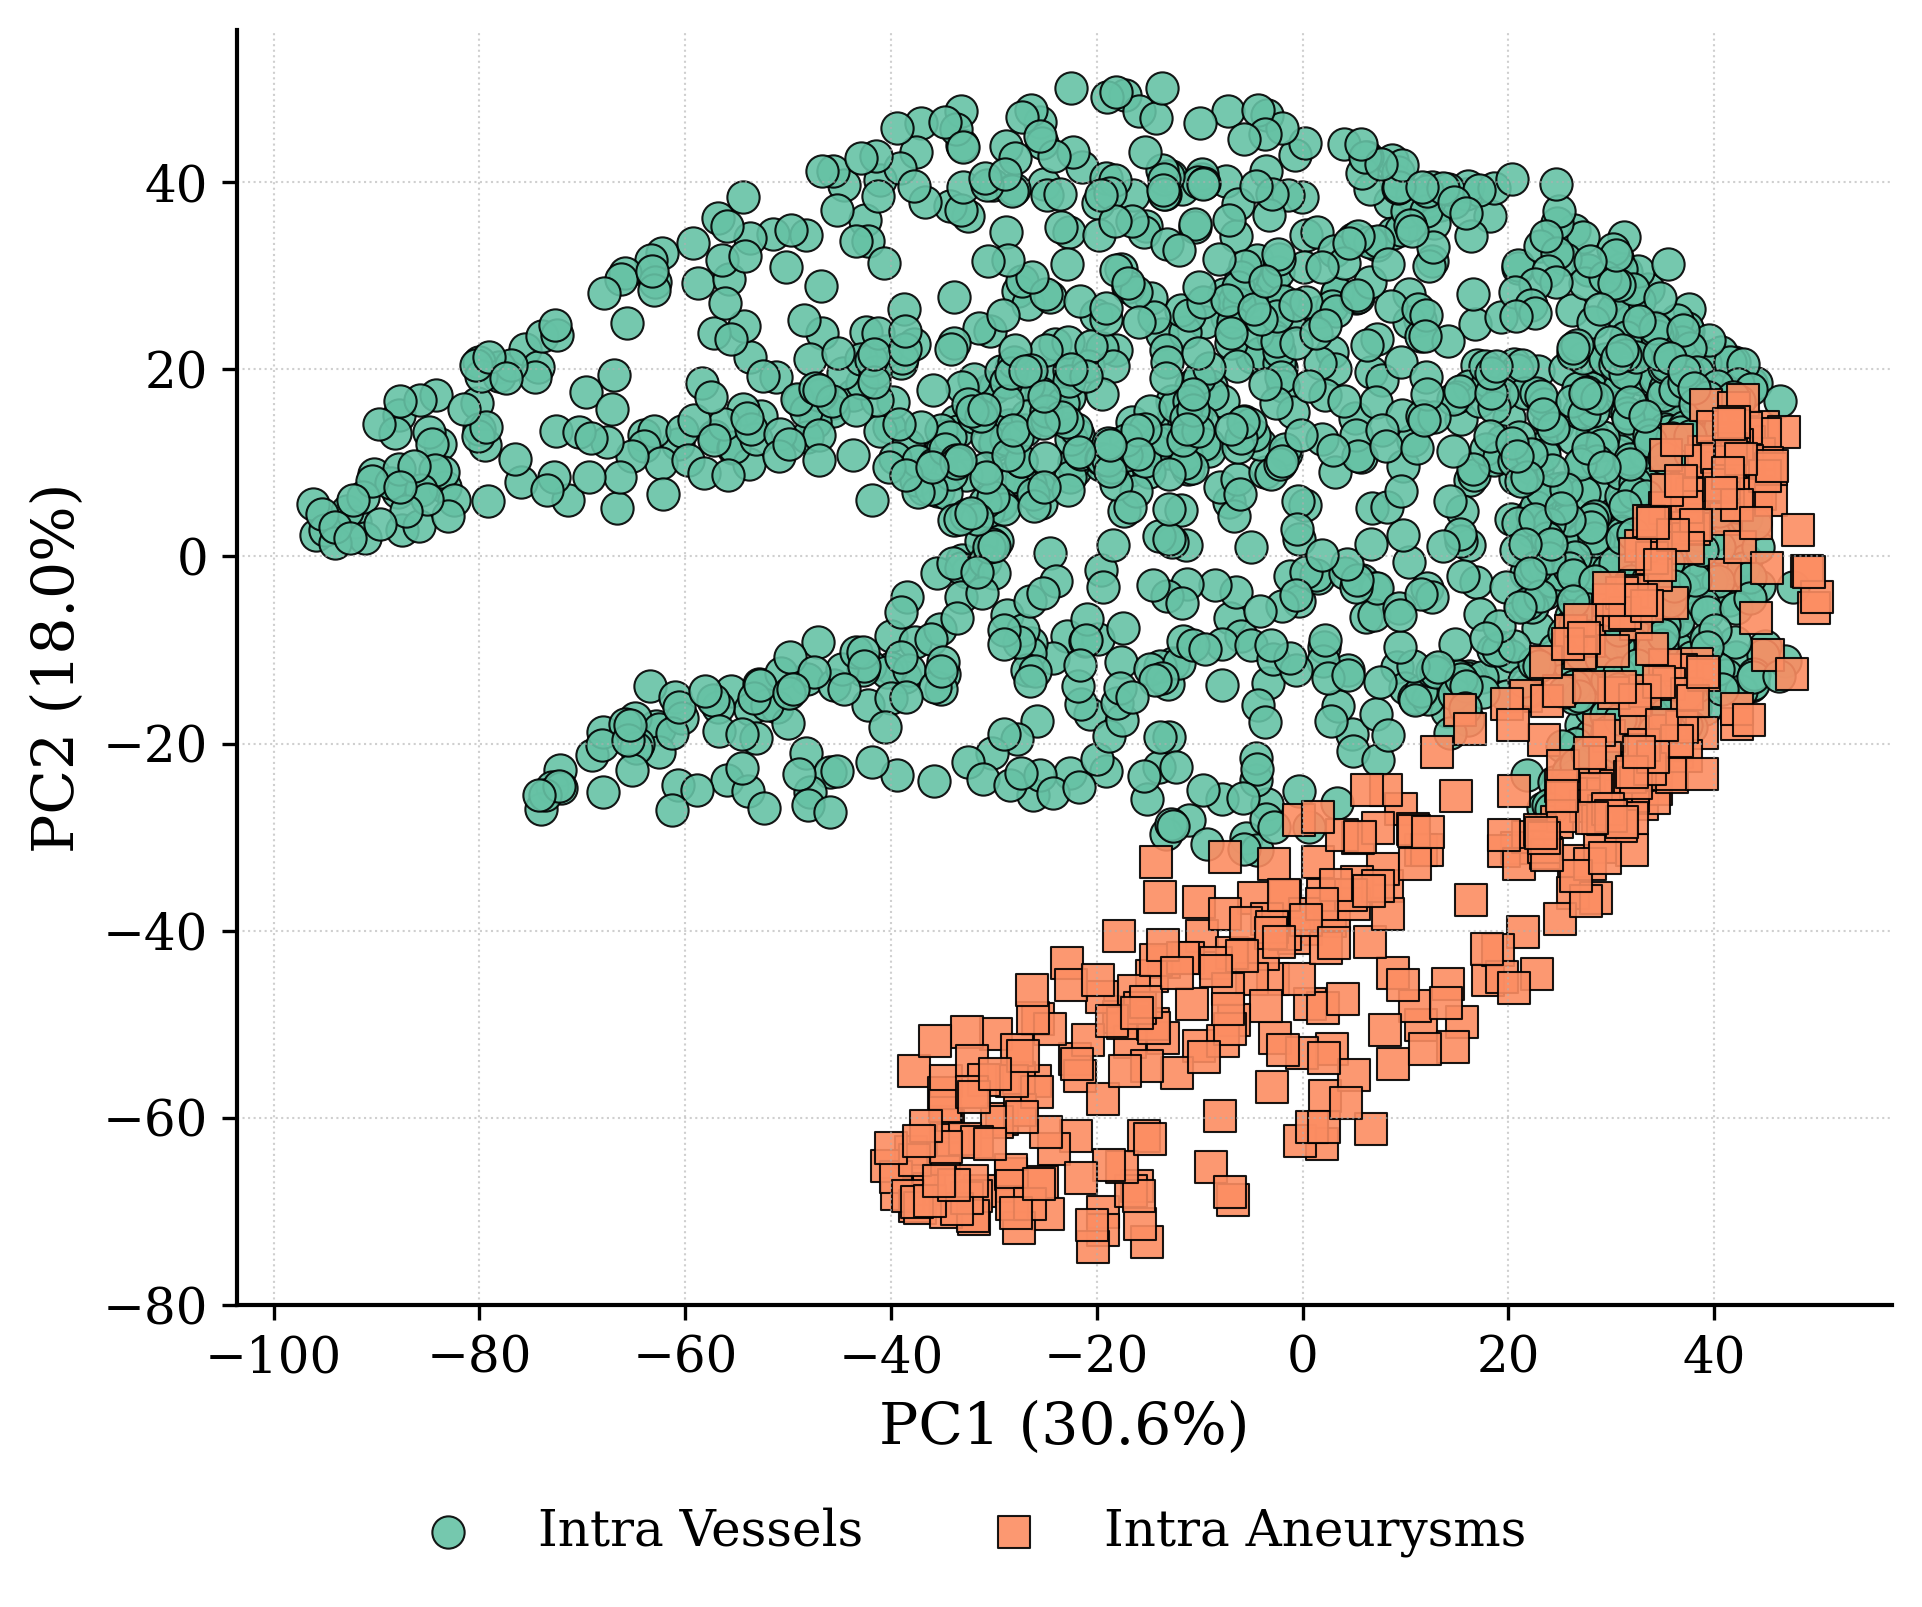
\includegraphics[width=0.47\textwidth]{pca_intra_features.png}
  \caption{Results of PCA on all the features from an annotated aneurysms from Intra3D \citep{yang2020intra}.}
  \label{fig:aneu_seg_2}
\end{figure}

Finally, we performed 2D PCA over the mean, standard deviation, minimum, and maximum of the features from each element of the AnXplore dataset. We then applied clustering algorithms to determine whether aneurysms within the same cluster exhibited similarities in shape and size. The optimal number of clusters for the 101 aneurysms was 15, and the results were revealing: within each cluster, aneurysms were generally similar in size and morphology, indicating that TRELLIS features are highly effective in capturing the geometric characteristics of 3D aneurysms. Results for the mean-based clusters are presented in Figure \ref{fig:clustering}. This suggests that, since aneurysms at higher risk of rupture tend to be larger and more irregular, the clustering output could be used to identify high-risk aneurysms. 

\begin{figure}[h!]
  \centering
  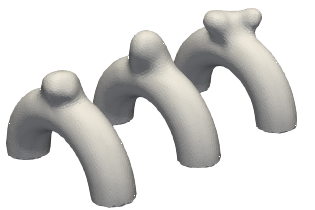
\includegraphics[width=0.20\textwidth]{cluster_11.png}
  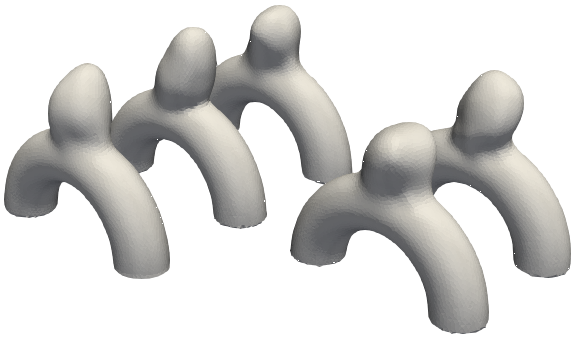
\includegraphics[width=0.27\textwidth]{cluster_13.png}
  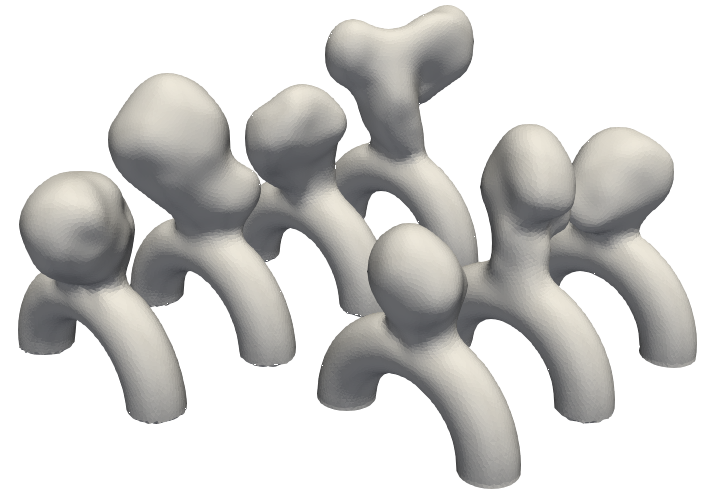
\includegraphics[width=0.28\textwidth]{cluster_14.png}
  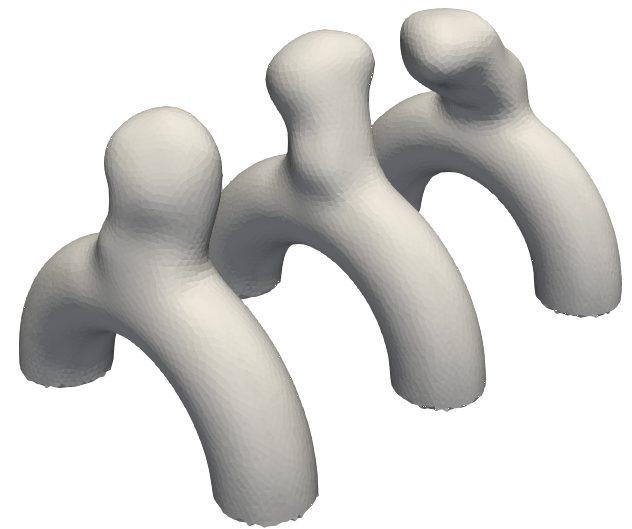
\includegraphics[width=0.18\textwidth]{cluster_6.png}
  \caption{Results of clustering on the AnXplore dataset using PCA on the mean features. The figure shows four clusters of aneurysms.}
  \label{fig:clustering}
\end{figure}



\section{Methodology} \label{METHODOLOGY}

\subsection{Classification}

Four methods were selected for the classification process: PointNet \citep{pointnet}, PointNet++ \citep{pointnetpp}, a simple MLP, and the direct application of PCA point clouds to train either an MLP or a logistic regression model. For the first two models, we trained them on the Intra3D dataset \citep{yang2020intra}, first using only the data provided by the dataset, and then with additional features from TRELLIS \citep{xiang2024structured} to compare the performance of both with identical neural networks. For the MLP, we performed a single training using only the features (without positions) to evaluate the performance of a very simple algorithm. For the two models with PCA, we directly used the four PCA point clouds with the mean, standard deviation, minimum, and maximum values.

For the PointNet \citep{pointnet} model, we did not use the original architecture but a slightly improved version, incorporating message passing to aggregate the features but not using the T-net module. For the baseline results, we used the positions from the point cloud combined with the surface normal vector at each point as features. We then ran the same algorithm but replaced the normals with the TRELLIS \citep{xiang2024structured} features at each point. The architecture consists of five modified PointNet layers, each with two layers of 64 neurons activated by ReLU (Rectified Linear Unit) functions. This is followed by a global max pooling layer and a linear layer of size 64 with an output of size 2, combined with a log softmax function. For each layer of message aggregation, the maximum number of neighbors is set to 16.

To implement PointNet++ \citep{pointnetpp}, we directly reused the original architecture. We followed the same approach as with PointNet: first using the point coordinates and normals, and then another run using the point coordinates and the TRELLIS \citep{xiang2024structured} features. The first layer is a set abstraction layer with an MLP consisting of one layer of 64 neurons and two layers of 128 neurons. The ratio for the farthest point sampling is set to 0.5, and the number of neighbors for the grouping phase is set to 64, within a radius of 0.2 (each element is rescaled to a normalized scale). The second layer is a set abstraction layer with two layers of 128 neurons and a final layer of size 256. The ratio for the farthest point sampling is set to 0.25, and the number of neighbors for the grouping phase is set to 64, within a radius of 0.4. Then, we have a global feature aggregation layer, using an MLP with one layer of 256 neurons, one layer of 512 neurons, and a final layer of size 1024. This is followed by a final MLP with one layer of 1024 neurons, one of 512 neurons, and an output layer of size 2. A dropout rate of 50\% is applied, and the output is passed through a log softmax function.

The MLP was trained using only the features of the points, not their positions. Each point has 8 features extracted from the mesh. We used simple MLP blocks to process these features and classify the points as aneurysms or healthy vessels. The MLP architecture is divided into two modules: the first processes the features for each point and is an MLP with one layer of 8 neurons (the number of features per point), one layer of 16 neurons, one layer of 8 neurons, and a final layer of size 1. The second module is a global MLP that processes the output of the first module; it has one layer whose size is the number of points sampled from the point cloud, one layer of 256 neurons, one layer of 64 neurons, one layer of 16 neurons, and an output layer of size 2, combined with a softmax function. The first module is shared between all points, and the second module is shared between all elements of the dataset. Both MLPs were trained using a 40\% dropout rate.  This architecture is shown in Figure \ref{fig:mlp_architecture}.

\begin{figure*}[t]
  \centering
  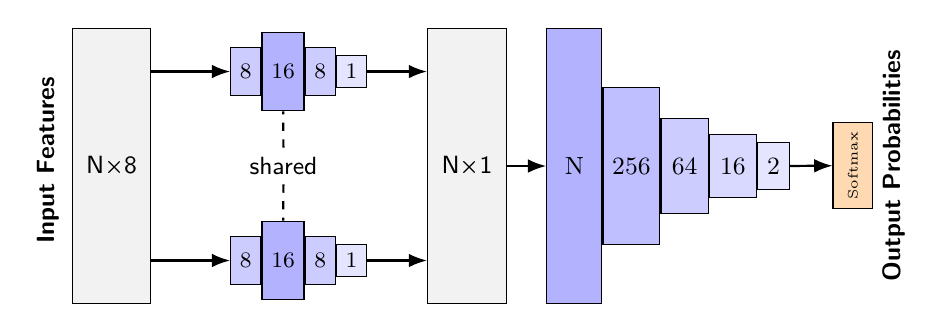
\begin{tikzpicture}[
 node distance=0.5cm and 0.5cm,
 layer/.style={draw, rectangle, minimum width=1cm, minimum height=3.5cm, fill=gray!10},
 softmax/.style={draw, rectangle, minimum width=1cm, minimum height=0.5cm, fill=orange!30},
 arrow/.style={-{Latex}, thick},
 simplearrow/.style={-, thick},
 font=\sffamily\small,
 scale=1,
 transform shape
 ]

  % Input block
  \node[layer] (nx64) {N×8};
  \node[left=0.2cm of nx64, rotate=90, xshift=1.25cm, yshift=0.1cm] (input) {\textbf{Input Features}};

  % Top MLP block
  \coordinate (mlp_top_anchor) at ($(nx64.east)+(1.0,1.2)$);
  \node[draw, minimum width=0.3cm, minimum height=0.6cm, fill=blue!20, anchor=west, font=\footnotesize] at (mlp_top_anchor) (shared_top_1) {8};
  \node[draw, minimum width=0.3cm, minimum height=1cm, fill=blue!30, right=0cm of shared_top_1, font=\footnotesize] (shared_top_2) {16};
  \node[draw, minimum width=0.3cm, minimum height=0.6cm, fill=blue!20, right=0cm of shared_top_2, font=\footnotesize] (shared_top_3) {8};
  \node[draw, minimum width=0.3cm, minimum height=0.3cm, fill=blue!10, right=0cm of shared_top_3, font=\footnotesize] (shared_top_4) {1};

  % Bottom MLP block
  \coordinate (mlp_bot_anchor) at ($(nx64.east)+(1.0,-1.2)$);
  \node[draw, minimum width=0.3cm, minimum height=0.6cm, fill=blue!20, anchor=west, font=\footnotesize] at (mlp_bot_anchor) (shared_bot_1) {8};
  \node[draw, minimum width=0.3cm, minimum height=1cm, fill=blue!30, right=0cm of shared_bot_1, font=\footnotesize] (shared_bot_2) {16};
  \node[draw, minimum width=0.3cm, minimum height=0.6cm, fill=blue!20, right=0cm of shared_bot_2, font=\footnotesize] (shared_bot_3) {8};
  \node[draw, minimum width=0.3cm, minimum height=0.1cm, fill=blue!10, right=0cm of shared_bot_3, font=\footnotesize] (shared_bot_4) {1};

  % Shared label centered between top and bottom MLP blocks
  \node[right=of nx64, xshift=-1.05cm] at ($(shared_top_2)!0.5!(shared_bot_2)$) (shared) {shared};

  % Aggregation layer
  \node[layer, right=3.5cm of nx64, yshift=0cm] (nx1024) {N×1};

  % Final MLP block split into layers
  \coordinate (mlp_final_anchor) at ($(nx1024.east)+(0.5,0)$);

  \node[draw, minimum width=0.7cm, minimum height=3.5cm, fill=blue!30, anchor=west, font=\small] at (mlp_final_anchor) (final_1) {N};
  \node[draw, minimum width=0.6cm, minimum height=2.0cm, fill=blue!25, right=0cm of final_1, font=\small] (final_2) {256};
  \node[draw, minimum width=0.6cm, minimum height=1.2cm, fill=blue!20, right=0cm of final_2, font=\small] (final_3) {64};
  \node[draw, minimum width=0.6cm, minimum height=0.8cm, fill=blue!15, right=0cm of final_3, font=\small] (final_4) {16};
  \node[draw, minimum width=0.4cm, minimum height=0.6cm, fill=blue!10, right=0cm of final_4, font=\small] (final_5) {2};

  % Softmax
  \node[softmax, right=of final_5, xshift=0.3cm, yshift=-0.55cm, rotate=90, font=\tiny] (softmax) {Softmax};
  \node[below=1cm of softmax, rotate=90, xshift=1.0cm] (output) {\textbf{Output Probabilities}};

  % Arrows from input to shared MLPs
  \draw[arrow] (nx64.east |- shared_top_1) -- (shared_top_1.west);
  \draw[arrow] (nx64.east |- shared_bot_1) -- (shared_bot_1.west);


  \draw[dashed, thick] (shared) -- (shared_bot_2);
  \draw[dashed, thick] (shared) -- (shared_top_2);

  % Arrows from shared MLPs to aggregation
  \draw[arrow] (shared_top_4.east) -- (nx1024.west |- shared_top_4);
  \draw[arrow] (shared_bot_4.east) -- (nx1024.west |- shared_bot_4);

  % Forward arrows
  \draw[arrow] (nx1024) -- (final_1);
  \draw[arrow] (final_5) -- (softmax);

  \end{tikzpicture}
  \caption{MLP Architecture for Point Cloud Classification with TRELLIS Encoding}
  \label{fig:mlp_architecture}
\end{figure*}

The three models were trained for 100 epochs with a batch size of 16. We used the AdamW optimizer with a learning rate of 0.001 and a cosine weight decay schedule.

For the algorithms using PCA, we trained an MLP and performed logistic regression on the 2D point clouds. For both, we tried using only the mean feature, then another training with mean and standard deviation, and finally one with all four metrics. This was done to show how well the features can represent the data type and to determine which metrics from the set of features for each element of the dataset are most useful. The architecture of the MLP is a first layer of size 8 (the number of features per point), a second layer of size 16, five layers of size 64, one layer of size 32, and a final layer of size 2. All layers are followed by ReLU activations and trained with a dropout rate of 40\%. The model was trained for 100 epochs with a learning rate of 0.01. Logistic regression was trained on the same data for 1000 iterations to ensure convergence.


\subsection{Segmentation}

For the segmentation process, we used two algorithms: PointNet \citep{pointnet} and PointNet++ \citep{pointnetpp}. For both, we adopted architectures similar to those used for classification. Specifically, for PointNet, we used the enhanced version, modifying the final layer for per-point segmentation instead of a global pooling layer. For PointNet++, we employed the original segmentation architecture. In both models, we compared performance using point clouds with surface normals as features, and then with TRELLIS features.

Our models were trained for 200 epochs for the algorithms without features, and only 100 with features, all with a batch size of 8. We used the AdamW optimizer with a learning rate of 0.001 and a cosine weight decay schedule. For the PointNet \citep{pointnet} architecture, we used five PointNet layers, each with two layers of 32 neurons with ReLU activations. The last layer is a linear layer of size 32 with an output of size 2, combined with a log softmax function. For each layer of message aggregation, the maximum number of neighbors is set to 16.

For PointNet++ \citep{pointnetpp}, the first layer is a set abstraction layer with three layers of 64 neurons and a final layer of size 128. The ratio for the farthest point sampling is set to 0.2, and the number of neighbors for the grouping phase is set to 64, within a radius of 0.2 (each element is rescaled to a normalized scale). The second layer is a set abstraction layer with three layers of 128 neurons and a final layer of size 256. The ratio for the farthest point sampling is set to 0.25, and the number of neighbors for the grouping phase is set to 64, within a radius of 0.4. Then, we have a global feature aggregation layer, using an MLP with one layer of 256 neurons, two layers of 512 neurons, and a final layer of size 1024. This is followed by three feature propagation modules: the first has three layers of 256 neurons, the second has a first layer of 128 neurons, a hidden layer of 256 neurons, and a final layer of size 128, and the last one has four layers of 128 neurons. Finally, each point is classified with a final MLP with three layers of 128 neurons and an output layer of size 2, combined with a log softmax function.

\subsection{Graph Neural Networks for Blood Flow Simulation}

For blood flow simulation, we used the AnXplore dataset \citep{anxplore} and the GNN architecture proposed in \citep{graphphysics}, without modifying the core architecture. The primary modification was the inclusion of surface features from TRELLIS \citep{xiang2024structured}, combined with the original mesh features for five runs, and five others without those features, repeating the process for different model sizes.

\section{Results} \label{RESULTS}

In this section, we present the results of our experiments on the Intra 3D dataset \citep{yang2020intra} and the AnXplore dataset \citep{anxplore}. We evaluate the performance of different models for classification, segmentation, and blood flow simulation. All classification and segmentation methods were evaluated using 5-fold cross-validation, and the results are reported as averages over the 5 folds.

The results of the classification experiments on the Intra 3D dataset \citep{yang2020intra} are shown in Table \ref{tab:classification_results}. We compare the performance of PointNet \citep{pointnet}, PointNet++ \citep{pointnetpp}, MLP, and PCA-based methods, with the best results from the Intra3D study \citep{yang2020intra} using PointNet++ \citep{pointnet} and PointCNN \citep{pointcnn}, and with the results from 3DMedPT \citep{yu20213dmedicalpointtransformer}. The results show that using TRELLIS features significantly improves the performance of both PointNet and PointNet++ compared to using only point coordinates and normals. The accuracy on vessels increases by approximately 7\%, the accuracy on aneurysms by approximately 70\% and the F1-score by between 10\% and 20\%, depending on the model. The MLP model also performs well when trained on TRELLIS features, achieving high accuracy.

Our best results are obtained with PointNet++ using TRELLIS features, reaching a vessel accuracy of 98.97\% and an F1 score of 97.82\%. The best model in terms of aneurysm accuracy is a simple MLP trained with TRELLIS features, achieving an aneurysm accuracy of 97.33\% and an F1 score of 95.32\%. These results show that with TRELLIS features, we can outperform state-of-the-art models on the Intra 3D dataset \citep{yang2020intra} in terms of accuracy on aneurysms and F1-score, even with classic neural networks and without relying on point cloud processing architectures.

\begin{table}[h]
  \centering
  \begin{tabular}{lcccc}
  \toprule
  \textbf{Model} & \textbf{Input} 
  & \textbf{V. (\%)} 
  & \textbf{A. (\%)} 
  & \textbf{F1} \\
  \midrule
  \multirow{3}{*}{MLP + feats}
    & 512 & 94.02 & 91.62 & 0.9261 \\
    & 1024 & 89.19 & \textbf{97.33} & 0.9532 \\
    & 2048 & 83.79 & 91.07 & 0.8625 \\ 
    \midrule
    \multirow{3}{*}{PointNet \citep{pointnet}}
    & 512 & 91.79 & 52.09 & 0.8209 \\
    & 1024 & 92.48 & 52.33 & 0.8274 \\
    & 2048 & 91.70 & 45.17 & 0.8019 \\
    \midrule
    \multirow{3}{*}{\shortstack{PointNet \citep{pointnet} \\+ feats}} 
    & 512 & 98.26 & 93.34 & 0.9116 \\
    & 1024 & 98.69 & 93.10 & 0.9742 \\
    & 2048 & 98.97 & 94.10 & \textbf{0.9782} \\
    \midrule
    \multirow{3}{*}{PointNet++ \citep{pointnetpp}}
    & 512 & 90.30 & 52.59 & 0.8130 \\
    & 1024 & 89.69 & 53.01 & 0.8106 \\
    & 2048 & 90.57 & 51.29 & 0.8105 \\
    \midrule
    \multirow{3}{*}{\shortstack{PointNet++ \citep{pointnetpp} \\+ feats}} 
    & 512 & 98.34 & 89.19 & 0.9618 \\
    & 1024 & 98.53 & 87.12 & 0.9589 \\
    & 2048 & 98.35 & 89.66 & 0.9632 \\
    \midrule
    \multirow{3}{*}{\shortstack{PointNet++ \citep{pointnetpp} \\(from \citep{yang2020intra})}} 
    & 512 & 98.52 & 86.69 & 0.8928 \\
    & 1024 & 98.52 & 88.51 & 0.9029 \\
    & 2048 & 98.76 & 87.31 & 0.9016 \\
    \midrule
    \multirow{3}{*}{\shortstack{PointCNN \citep{pointcnn} \\(from \citep{yang2020intra})}} 
    & 512 & 98.38 & 78.25 & 0.8494 \\
    & 1024 & 98.79 & 81.28 & 0.8748 \\
    & 2048 & 98.95 & 85.81 & 0.9044 \\
    \midrule
    \multirow{3}{*}{\shortstack{3DMedPT \citep{yu20213dmedicalpointtransformer}}} 
    & 512 & 99.02 & 94.06 & 0.920 \\
    & 1024 & 99.24 & 93.26 & 0.936 \\
    & 2048 & 99.07 & 93.49 & 0.931 \\
    \midrule  
    \midrule
    \multirow{3}{*}{MLP on PCA} 
    & mean & \textbf{100} & 51.56 & 0.8766 \\
    & mean and std& 99.56 & 68.44 & 0.9201 \\
    & all metrics & 98.70 & 78.07 & 0.9382 \\
    \midrule
    \multirow{3}{*}{\shortstack{Logistic Regression \\ on PCA}}    
    & mean & 96.43 & 65.40 & 0.8896 \\
    & mean and std & 98.61 & 73.83 & 0.9273 \\
    & all metrics & 98.00 & 75.64 & 0.9271 \\
  \bottomrule
  \end{tabular}
  \caption{Comparison of the different models for classification on the Intra 3D dataset. Results are mean values for vessel segment accuracy (V.), aneurysm segment accuracy (A.), and F1-score.}
  \label{tab:classification_results}
\end{table}

The segmentation results on the Intra 3D dataset \citep{yang2020intra} are shown in Table \ref{tab:segmentation_results}. We compare the performance of PointNet \citep{pointnet} and PointNet++ \citep{pointnetpp} models, both with and without TRELLIS features, with the best results from the Intra3D study \citep{yang2020intra} using PointNet++ \citep{pointnetpp} and SO-net \citep{sonet}, and with the results from 3DMedPT \citep{yu20213dmedicalpointtransformer}. The results indicate that both models achieve high accuracy in segmenting aneurysms and healthy vessels. The addition of TRELLIS features consistently leads to notable improvements in segmentation performance.

Our best results are achieved with PointNet using TRELLIS features and using 2048 points. The difference between models using only the original features (point coordinates and normals) and those using TRELLIS features is clear. Also, all the algorithm using TRELLIS features outperform the best results from the Intra3D study \citep{yang2020intra} and 3DMedPT \citep{yu20213dmedicalpointtransformer} for all metrics, including IoU (Intersection of Union) and DSC (Dice Similarity Coefficient).
The results show that TRELLIS features significantly enhance the segmentation performance of both PointNet and PointNet++. 

\begin{table}[h]
  \footnotesize
  \centering
  \begin{tabular}{lcccccc}
  \toprule
  \textbf{Model} & \textbf{Points} 
  & \textbf{IoU V.} 
  & \textbf{IoU A.} 
  & \textbf{DSC V.}
  & \textbf{DSC A.} \\
  \midrule
  \multirow{3}{*}{PointNet \citep{pointnet}}
  & 512 & 88.08 & 66.38 & 93.65 & 79.75 \\
  & 1024 & 85.81 & 60.17 & 92.18 & 75.09 \\
  & 2048 & 81.16 & 50.95 & 89.59 & 67.19 \\ 
  \midrule
  \multirow{3}{*}{\shortstack{PointNet \citep{pointnet} \\+ feats}}
  & 512 & 95.84 & 86.53 & 97.87 & 92.77 \\
  & 1024 & 96.53 & 88.59 & 98.23 & 93.94 \\
  & 2048 & \textbf{96.57} & \textbf{88.67} & \textbf{98.26} & \textbf{93.99} \\
  \midrule
  \multirow{3}{*}{PointNet++ \citep{pointnetpp}}
  & 512 & 87.87 & 64.75 & 93.52 & 78.50 \\
  & 1024 & 88.52 & 66.68 & 93.91 & 79.90 \\
  & 2048 & 89.33 & 67.98 & 94.30 & 80.89 \\
  \midrule
  \multirow{3}{*}{\shortstack{PointNet++ \citep{pointnetpp} \\+ feats}}
  & 512 & 96.12 & 87.19 & 98.03 & 93.14 \\
  & 1024 & 96.38 & 88.09 & 98.15 & 93.66 \\
  & 2048 & 96.46 & 88.31 & 98.20 & 93.78 \\
  \midrule
  \multirow{3}{*}{\shortstack{PointNet++ \citep{pointnetpp} \\ (from \citep{yang2020intra})}}
  & 512 & 93.34 & 76.22 & 96.48 & 83.92 \\
  & 1024 & 93.35 & 76.38 & 96.47 & 84.62 \\ 
  & 2048 & 93.24 & 76.21 & 96.40 & 84.64 \\
  \midrule
  \multirow{3}{*}{\shortstack{SO-net \citep{sonet} \\ (from \citep{yang2020intra})}}
  & 512 & 94.22 & 80.14 & 96.95 & 87.90 \\
  & 1024 & 94.42 & 80.99 & 97.06 & 88.41 \\
  & 2048 & 94.46 & 81.40 & 97.09 & 88.76 \\
  \midrule
  \multirow{3}{*}{\shortstack{3DMedPT \citep{yu20213dmedicalpointtransformer}}}
  & 512 & 94.82 & 81.80 & 97.29 & 89.25 \\
  & 1024 & 94.76 & 82.39 & 97.25 & 89.71 \\
  & 2048 & 93.52 & 80.13 & 96.59 & 88.69 \\
  \bottomrule
  \end{tabular}
  \caption{Comparison of the different models for segmentation on the Intra 3D dataset. Results are mean values for IoU (Intersection of Union) and DSC (Dice Similarity Coefficient) on vessels (V.) and aneurysms (A.).}
  \label{tab:segmentation_results}
\end{table}

The results of the GNN + Transformers model \citep{graphphysics} on the AnXplore dataset \citep{anxplore} are shown in Table \ref{tab:gnn_results}. The model was trained using the features extracted from TRELLIS \citep{xiang2024structured} and the mesh structure of the aneurysms. The results indicate that the model achieves a lower RMSE (Root Mean Square Error) across all time steps of the blood flow simulation with the addition of TRELLIS features compared to using only the original features (point coordinates and normals). The error is reduced by approximately 15\%, demonstrating the effectiveness of these features for simulating blood flow.

\begin{table}[h]
  \centering
  \setlength{\tabcolsep}{1.06em} % Increase column separation
  \renewcommand{\arraystretch}{1.12} % Increase row height
  \begin{tabular}{lcc}
  \toprule
  \multirow{2}{*}{\textbf{Model}} & \multicolumn{2}{c}{\textbf{All-Rollout RMSE}} \\
  \cmidrule(lr){2-3}
  & \textbf{Mean} & \textbf{Std} \\
  \midrule
 S/1 & 7.57 & 1.103 \\
  \midrule
 S/1 + feats & 6.09 & 0.637 \\
  \midrule
 L/1 & 4.03 & 0.330 \\
  \midrule
 L/1 + feats & \textbf{3.55} & \textbf{0.017} \\
  \bottomrule
  \end{tabular}
  \caption{Results of the GNN + Transformers model on the AnXplore dataset. The All-Rollout RMSE is computed over all time steps of the blood flow simulation.}
  \label{tab:gnn_results}
\end{table}


Additionally, this approach impacts the training time for the models. For point cloud processing, using the MLP allows us to reduce the training time by a factor of three compared to models like PointNet and PointNet++.

Another important aspect is the encoding time: encoding 400 objects with TRELLIS on an A100 GPU takes about 12 hours, which averages to five minutes per object. While this is a significant amount of time, it is a one-time process—after encoding, we can train different models on the resulting dataset. In comparison, running the entire pipeline of encoding and training on the full dataset would increase the total time by a factor of 30 compared to training point cloud processing models such as PointNet or PointNet++ alone.

\section{Conclusion} \label{CONCLUSION}
\todo{Recheck every bib/doi}
In this work, we explored the use of TRELLIS \citep{xiang2024structured} features for 3D medical object classification and segmentation tasks, specifically on the Intra 3D dataset \citep{yang2020intra} and the AnXplore dataset \citep{anxplore}. We showed that using TRELLIS features significantly improves the performance of PointNet \citep{pointnet} and PointNet++ \citep{pointnetpp} compared to using only point coordinates and normals. The results indicate that TRELLIS features enhance the classification accuracy on aneurysms and vessels, achieving state-of-the-art performance on the Intra 3D dataset \citep{yang2020intra}.

We also applied TRELLIS features to the AnXplore dataset \citep{anxplore} for blood flow simulation using Graph Neural Networks (GNNs), demonstrating the versatility of these features for different 3D tasks.

Moreover, we found that a simple MLP trained on TRELLIS features achieves competitive results, outperforming state-of-the-art models on the Intra 3D dataset \citep{yang2020intra}. We also analyzed the TRELLIS features, showing that they effectively capture the shape and size of aneurysms, enabling clustering based on these characteristics, which could support the identification of aneurysms at risk of rupture.

Overall, we conclude that TRELLIS features are a powerful tool for 3D medical data, for classification, segmentation, and blood flow simulation, and offer a promising direction for future research in this area. Our study demonstrates that TRELLIS encoding is a highly effective method for extracting features from 3D medical objects, even though the encoder was not originally trained on this type of data. The ability to encode complex 3D structures into meaningful features opens up new possibilities for improving the performance of various 3D models.

For future work, it would be interesting to apply TRELLIS features to other 3D object classification or segmentation tasks. For instance, PointNet or PointNet++ could be evaluated on different 3D object datasets. Comparing results across these datasets could help assess how well TRELLIS features generalize to various types of 3D objects and tasks. Additionally, testing other models such as SO-net \citep{sonet} or PointCNN \citep{pointcnn} with TRELLIS features could provide further insights into their effectiveness across different architectures.

To address the encoding time, a more detailed study could be conducted to determine how much the number of views can be reduced without significantly degrading the performance of the classification and segmentation models.

\onecolumngrid

\bibliographystyle{unsrtnat}
\bibliography{biblio}

\appendix

\clearpage
\section{Comparisons of the Performances of the Different Models}
\label{annexeA}

\begin{table}[h]
  \centering
  \begin{tabular}{llccccccc}
  \toprule
  \textbf{Model} & \textbf{Features} & \textbf{Input} 
  & \multicolumn{2}{c}{\textbf{V. (\%)}} 
  & \multicolumn{2}{c}{\textbf{A. (\%)}} 
  & \multicolumn{2}{c}{\textbf{F1}} \\
  \cmidrule(lr){4-5} \cmidrule(lr){6-7} \cmidrule(lr){8-9}
  & & & mean & std & mean & std & mean & std \\
  \midrule
  \multirow{3}{*}{MLP} & \multirow{3}{*}{with}
  & 512 & 94.02 & 8.93 & 91.62 & 4.28 & 0.9261 & 0.0577 \\
  &  & 1024 & 89.19 & 2.62 & \textbf{97.33} & 8.72 & 0.9532 & 0.0220 \\
  &  & 2048 & 83.79 & 14.55 & 91.07 & 12.70 & 0.8625 & 0.0877 \\ 
  \midrule
  \multirow{3}{*}{PointNet \citep{pointnet}} & \multirow{3}{*}{without}
  & 512 & 91.79 & 3.26 & 52.09 & 8.59 & 0.8209 & 0.0280 \\
  &  & 1024 & 92.48 & 2.06 & 52.33 & 4.52 & 0.8274 & 0.0059 \\
  &  & 2048 & 91.70 & 1.90 & 45.17 & 5.93 & 0.8019 & 0.0165 \\
  \midrule
  \multirow{3}{*}{PointNet \citep{pointnet}} & \multirow{3}{*}{with}
  & 512 & 98.26 & 0.79 & 93.34 & 3.41 & 0.9116 & 0.0109 \\
  &  & 1024 & 98.69 & 0.55 & 93.10 & \textbf{1.76} & 0.9742 & \textbf{0.0052} \\
  &  & 2048 & 98.97 & 0.71 & 94.10 & 5.86 & \textbf{0.9782} & 0.0177\\
  \midrule
  \multirow{3}{*}{PointNet++ \citep{pointnetpp}} & \multirow{3}{*}{without}
  & 512 & 90.30 & 2.04 & 52.59 & 2.61 & 0.8130 & 0.0124\\
  &  & 1024 & 89.69 & 2.23 & 53.01 & 2.36 & 0.8106 & 0.0123 \\
  &  & 2048 & 90.57 & 2.28 & 51.29 & 4.49 & 0.8105 & 0.0155 \\
  \midrule
  \multirow{3}{*}{PointNet++ \citep{pointnetpp}} & \multirow{3}{*}{with}
  & 512 & 98.34 & 0.94 & 89.19 & 4.61 & 0.9618 & 0.0147 \\
  &  & 1024 & 98.53 & 0.77 & 87.12 & 5.02 & 0.9589 & 0.0108 \\
  &  & 2048 & 98.35 & 0.92 & 89.66 & 3.35 & 0.9632 & 0.0090\\
  \midrule
  \multirow{3}{*}{\shortstack{PointNet++ \citep{pointnetpp} \\(from \citep{yang2020intra})}} & \multirow{3}{*}{without}
  & 512 & 98.52 & - & 86.69 & - & 0.8928 & -\\
  & & 1024 & 98.52 & - & 88.51 & - & 0.9029 & - \\
  & & 2048 & 98.76 & - & 87.31 & - & 0.9016 & - \\
  \midrule
  \multirow{3}{*}{\shortstack{PointCNN \citep{pointcnn} \\(from \citep{yang2020intra})}} & \multirow{3}{*}{without}
  & 512 & 98.38 & - & 78.25 & - & 0.8494 & -  \\
  & & 1024 & 98.79 & - & 81.28 & - & 0.8748 & - \\
  & & 2048 & 98.95 & - & 85.81 & - & 0.9044 & - \\
  \midrule
  \multirow{3}{*}{\shortstack{3DMedPT \citep{yu20213dmedicalpointtransformer}}} & \multirow{3}{*}{without}
  & 512 & 99.02 & - & 94.06 & - & 0.920 & -  \\
  & & 1024 & 99.24 & - & 93.26 & - & 0.936 & - \\
  & & 2048 & 99.07 & - & 93.49 & - & 0.931 & - \\
  \midrule
  \midrule
  \multirow{3}{*}{MLP on PCA} 
  & mean & & \textbf{100} & \textbf{0.00} & 51.56 & 9.21 & 0.8766 & 0.0273\\
  & mean and std& & 99.56 & 0.39 & 68.44 & 9.10 & 0.9201 & 0.0221\\
  & all metrics & & 98.70 & 1.58 & 78.07 & 8.55 & 0.9382 & 0.0203\\
  \midrule
  \multirow{3}{*}{\shortstack{Logistic Regression \\ on PCA}}    
  & mean & & 96.43 & 1.08 & 65.40 & 5.74 & 0.8896 & 0.0139\\
  & mean and std & & 98.61 & 0.70 & 73.83 & 4.63 & 0.9273 & 0.0121\\
  & all metrics & & 98.00 & 0.44 & 75.64 & 7.07 & 0.9271 & 0.0180 \\
  \bottomrule
  \end{tabular}
  \caption{Full comparison of the different models for classification on the Intra 3D dataset. Results are mean and standard deviation (std) on vessels segment accuracy (V.), aneurysms segment accuracy (A.), and F1-score.}
  \label{tab:classification_results_complete}
\end{table}

\begin{table}[h]
  \centering
  \begin{tabular}{llccccccccc}
  \toprule
  \textbf{Model} & \textbf{Features} & \textbf{Input} 
  & \multicolumn{2}{c}{\textbf{IoU V. (\%)}} 
  & \multicolumn{2}{c}{\textbf{IoU A. (\%)}} 
  & \multicolumn{2}{c}{\textbf{DSC V. (\%)}}
  & \multicolumn{2}{c}{\textbf{DSC A. (\%)}} \\
  \cmidrule(lr){4-5} \cmidrule(lr){6-7} \cmidrule(lr){8-9} \cmidrule(lr){10-11}
  & & & mean & std & mean & std & mean & std & mean & std \\
  \midrule
  \multirow{3}{*}{PointNet \citep{pointnet}} & \multirow{3}{*}{without}
  & 512 & 88.08 & 1.74 & 66.38 & 3.84 & 93.65 & 0.99 & 79.75 & 2.54 \\
  &  & 1024 & 85.81 & 1.13 & 60.17 & 3.31 & 92.18 & 0.66 & 75.09 & 2.64 \\
  &  & 2048 & 81.16 & 2.04 & 50.95 & 7.97 & 89.59 & 1.26 & 67.19 & 7.45 \\ 
  \midrule
  \multirow{3}{*}{PointNet \citep{pointnet}} & \multirow{3}{*}{with}
  & 512 & 95.84 & 0.37 & 86.53 & 2.40 & 97.87 & 0.16 & 92.77 & 1.29 \\
  &  & 1024 & 96.53 & 0.41 & 88.59 & 1.86 & 98.23 & 0.22 & 93.94 & 1.05 \\
  &  & 2048 & \textbf{96.57} & 0.28 & \textbf{88.67} & \textbf{1.82} & \textbf{98.26} & 0.15 & \textbf{93.99} & \textbf{1.03} \\
  \midrule
  \multirow{3}{*}{PointNet++ \citep{pointnetpp}} & \multirow{3}{*}{without}
  & 512 & 87.87 & 2.80 & 64.75 & 5.50 & 93.52 & 1.62 & 78.50 & 4.05 \\
  &  & 1024 & 88.52 & 1.08 & 66.68 & 5.67 & 93.91 & 0.60 & 79.90 & 4.17\\
  &  & 2048 & 89.33 & 1.21 & 67.98 & 3.69 & 94.30 & 0.68 & 80.89 & 2.60\\
  \midrule
  \multirow{3}{*}{PointNet++ \citep{pointnetpp}} & \multirow{3}{*}{with}
  & 512 & 96.13 & 0.44 & 87.19 & 2.62 & 98.03 & 0.23 & 93.14 & 1.52 \\
  &  & 1024 & 96.38 & \textbf{0.22} & 88.09 & 2.17 & 98.15 & \textbf{0.11} & 93.66 & 1.23 \\
  &  & 2048 & 96.46 & 0.40 & 88.31 & 2.51 & 98.20 & 0.21 & 93.78 & 1.43 \\
  \midrule
  \multirow{3}{*}{\shortstack{PointNet++ \citep{pointnetpp} \\ (from \citep{yang2020intra})}} & \multirow{3}{*}{without}
  & 512 & 93.34 & 1.28 & 76.22 & 4.85 & 96.48 & 0.73 & 83.92 & 4.34 \\
  & & 1024 & 93.35 & 1.15 & 76.38 & 4.36 &96.47 & 0.65 & 84.62 & 3.82 \\ 
  & & 2048 & 93.24 & 1.18 & 76.21 & 4.34 & 96.40 & 0.67 & 84.64 & 3.77 \\
  \midrule
  \multirow{3}{*}{\shortstack{SO-net \citep{sonet} \\ (from \citep{yang2020intra})}} & \multirow{3}{*}{without}
  & 512 & 94.22 & 1.07 & 80.14 & 3.28 & 96.95 & 0.59 & 87.90 & 2.43 \\
  &  & 1024 & 94.42 & 1.04 & 80.99 & 3.21 & 97.06 & 0.58 & 88.41 & 2.43 \\
  &  & 2048 & 94.46 & 1.00 & 81.40 & 3.09 & 97.09 & 0.55 & 88.76 & 2.24 \\
  \midrule
  \multirow{3}{*}{\shortstack{3DMedPT \citep{yu20213dmedicalpointtransformer}}} & \multirow{3}{*}{without}
  & 512 & 94.82 & - & 81.80 & - & 97.29 & - & 89.25 & - \\
  & & 1024 & 94.76 & - & 82.39 & - & 97.25 & - & 89.71 & - \\
  & & 2048 & 93.52 & - & 80.13 & - & 96.59 & - & 88.69 & - \\
  \bottomrule
  \end{tabular}
  \caption{Full comparison of the different models for segmentation on the Intra 3D dataset. Results are mean and standard deviation (std) on vessels segment accuracy (V.), aneurysms segment accuracy (A.), and F1-score.}
  \label{tab:segmentation_results_complete}
\end{table}


\clearpage
\section{Supplementary figures on the analysis of the TRELLIS features}
\label{annexeB}

\vspace{-0.3cm}

\begin{figure}[h!]
  \centering
  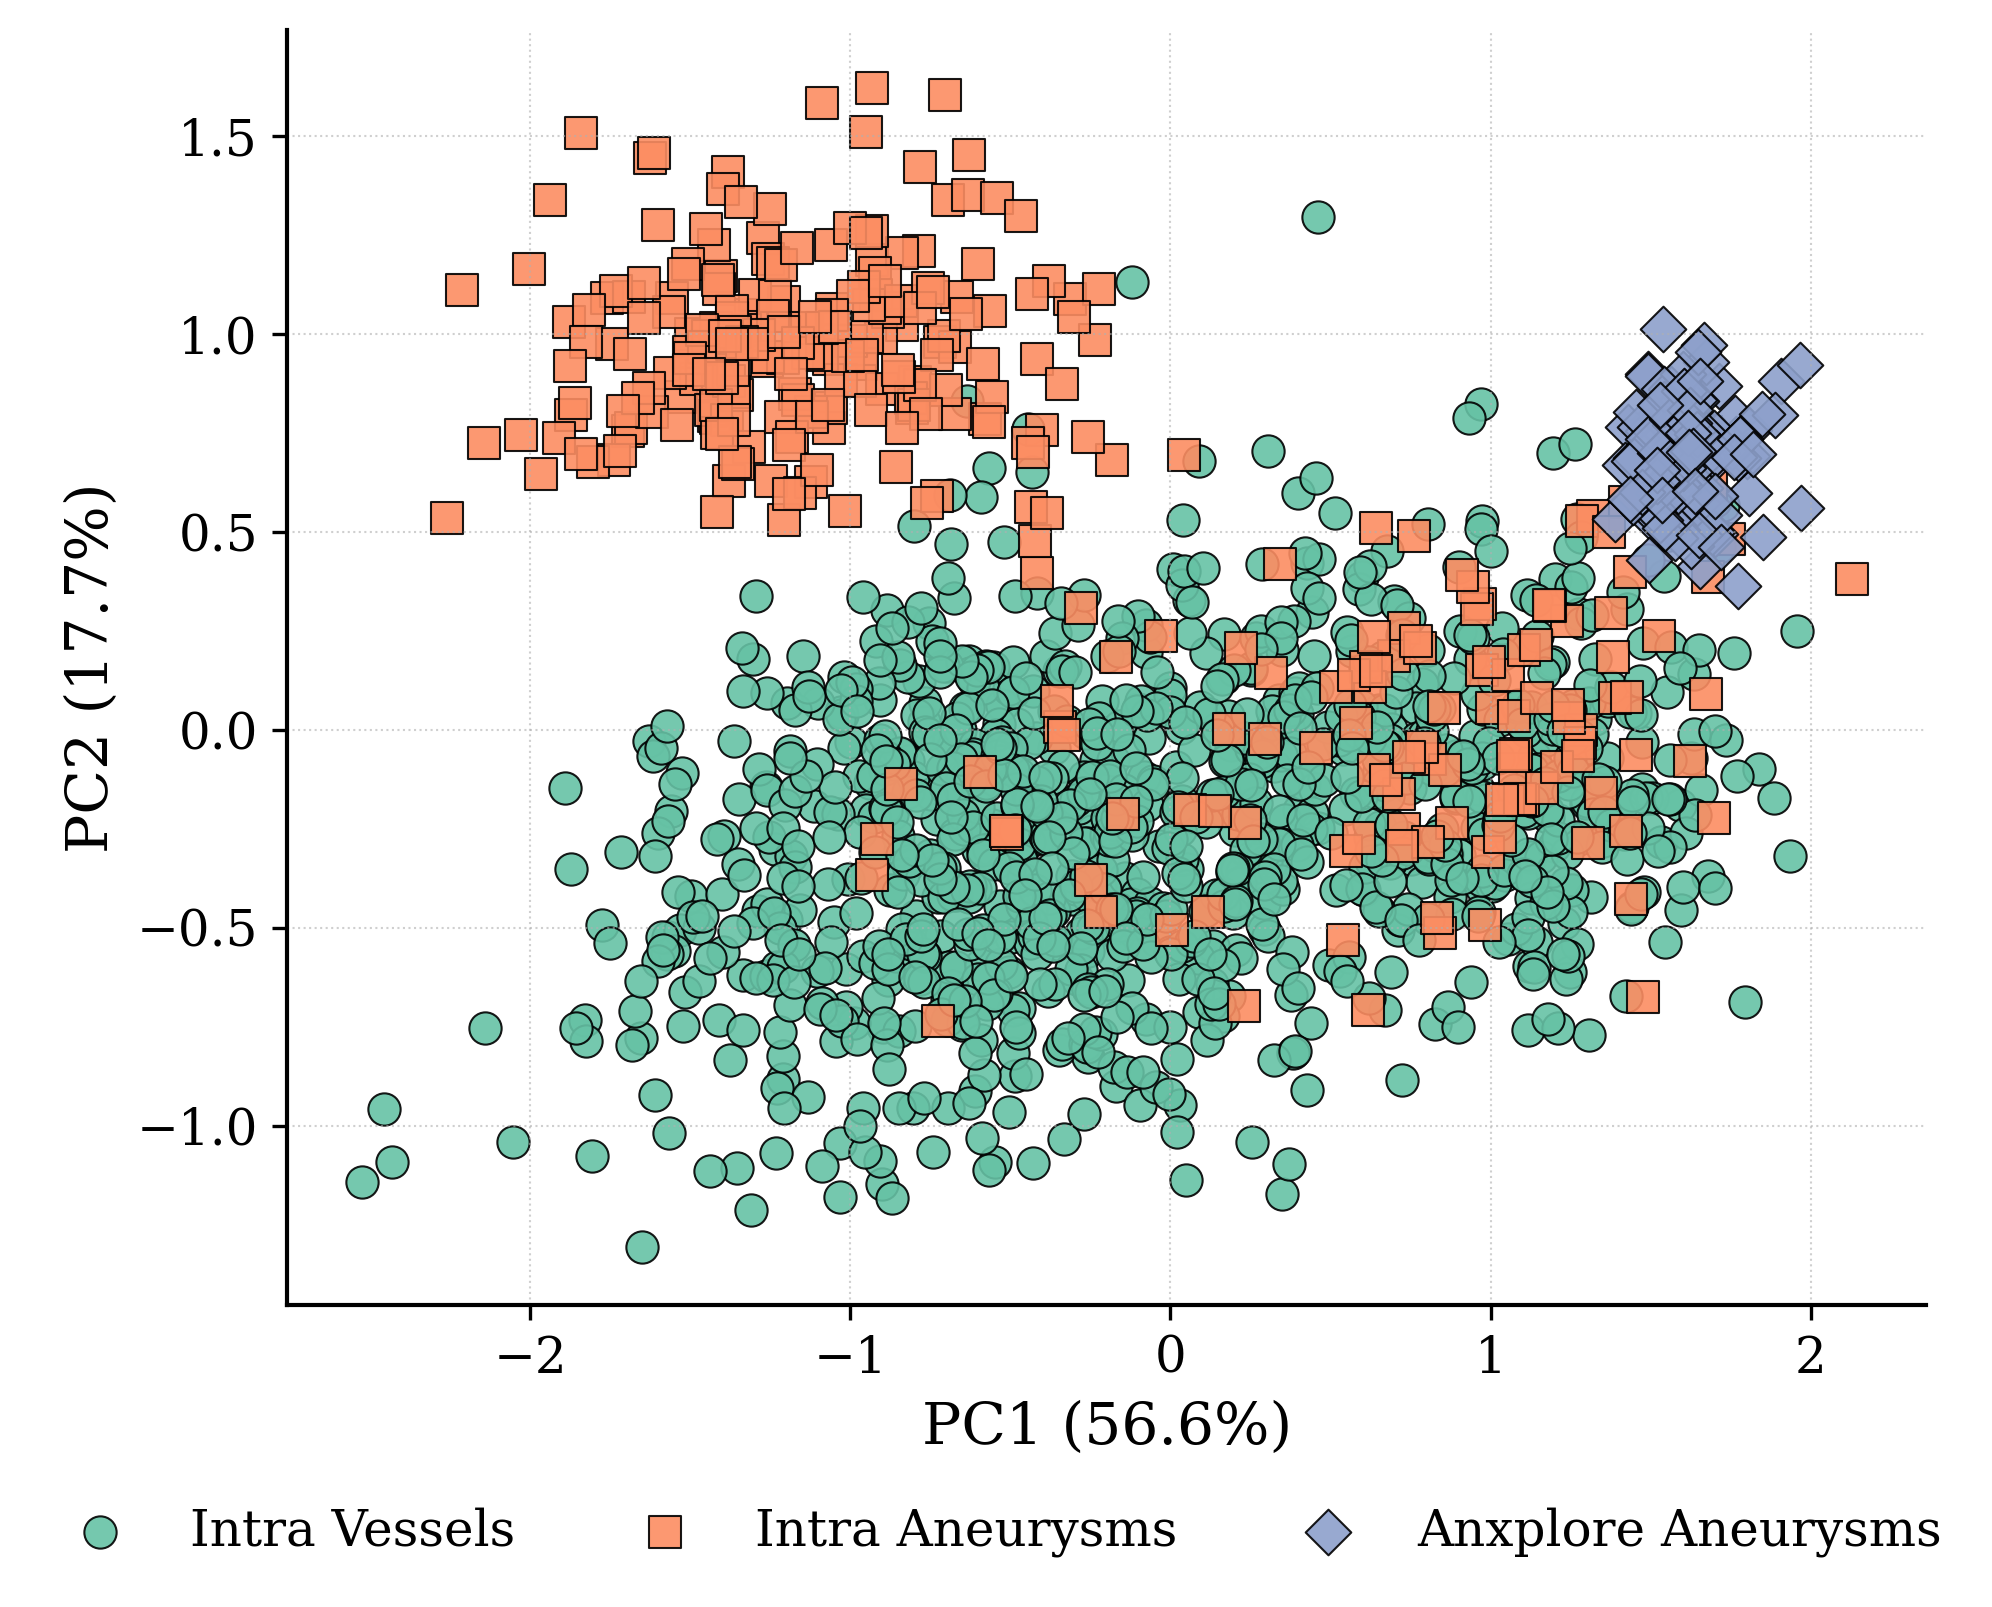
\includegraphics[width=0.33\textwidth]{pca_mean.png}
  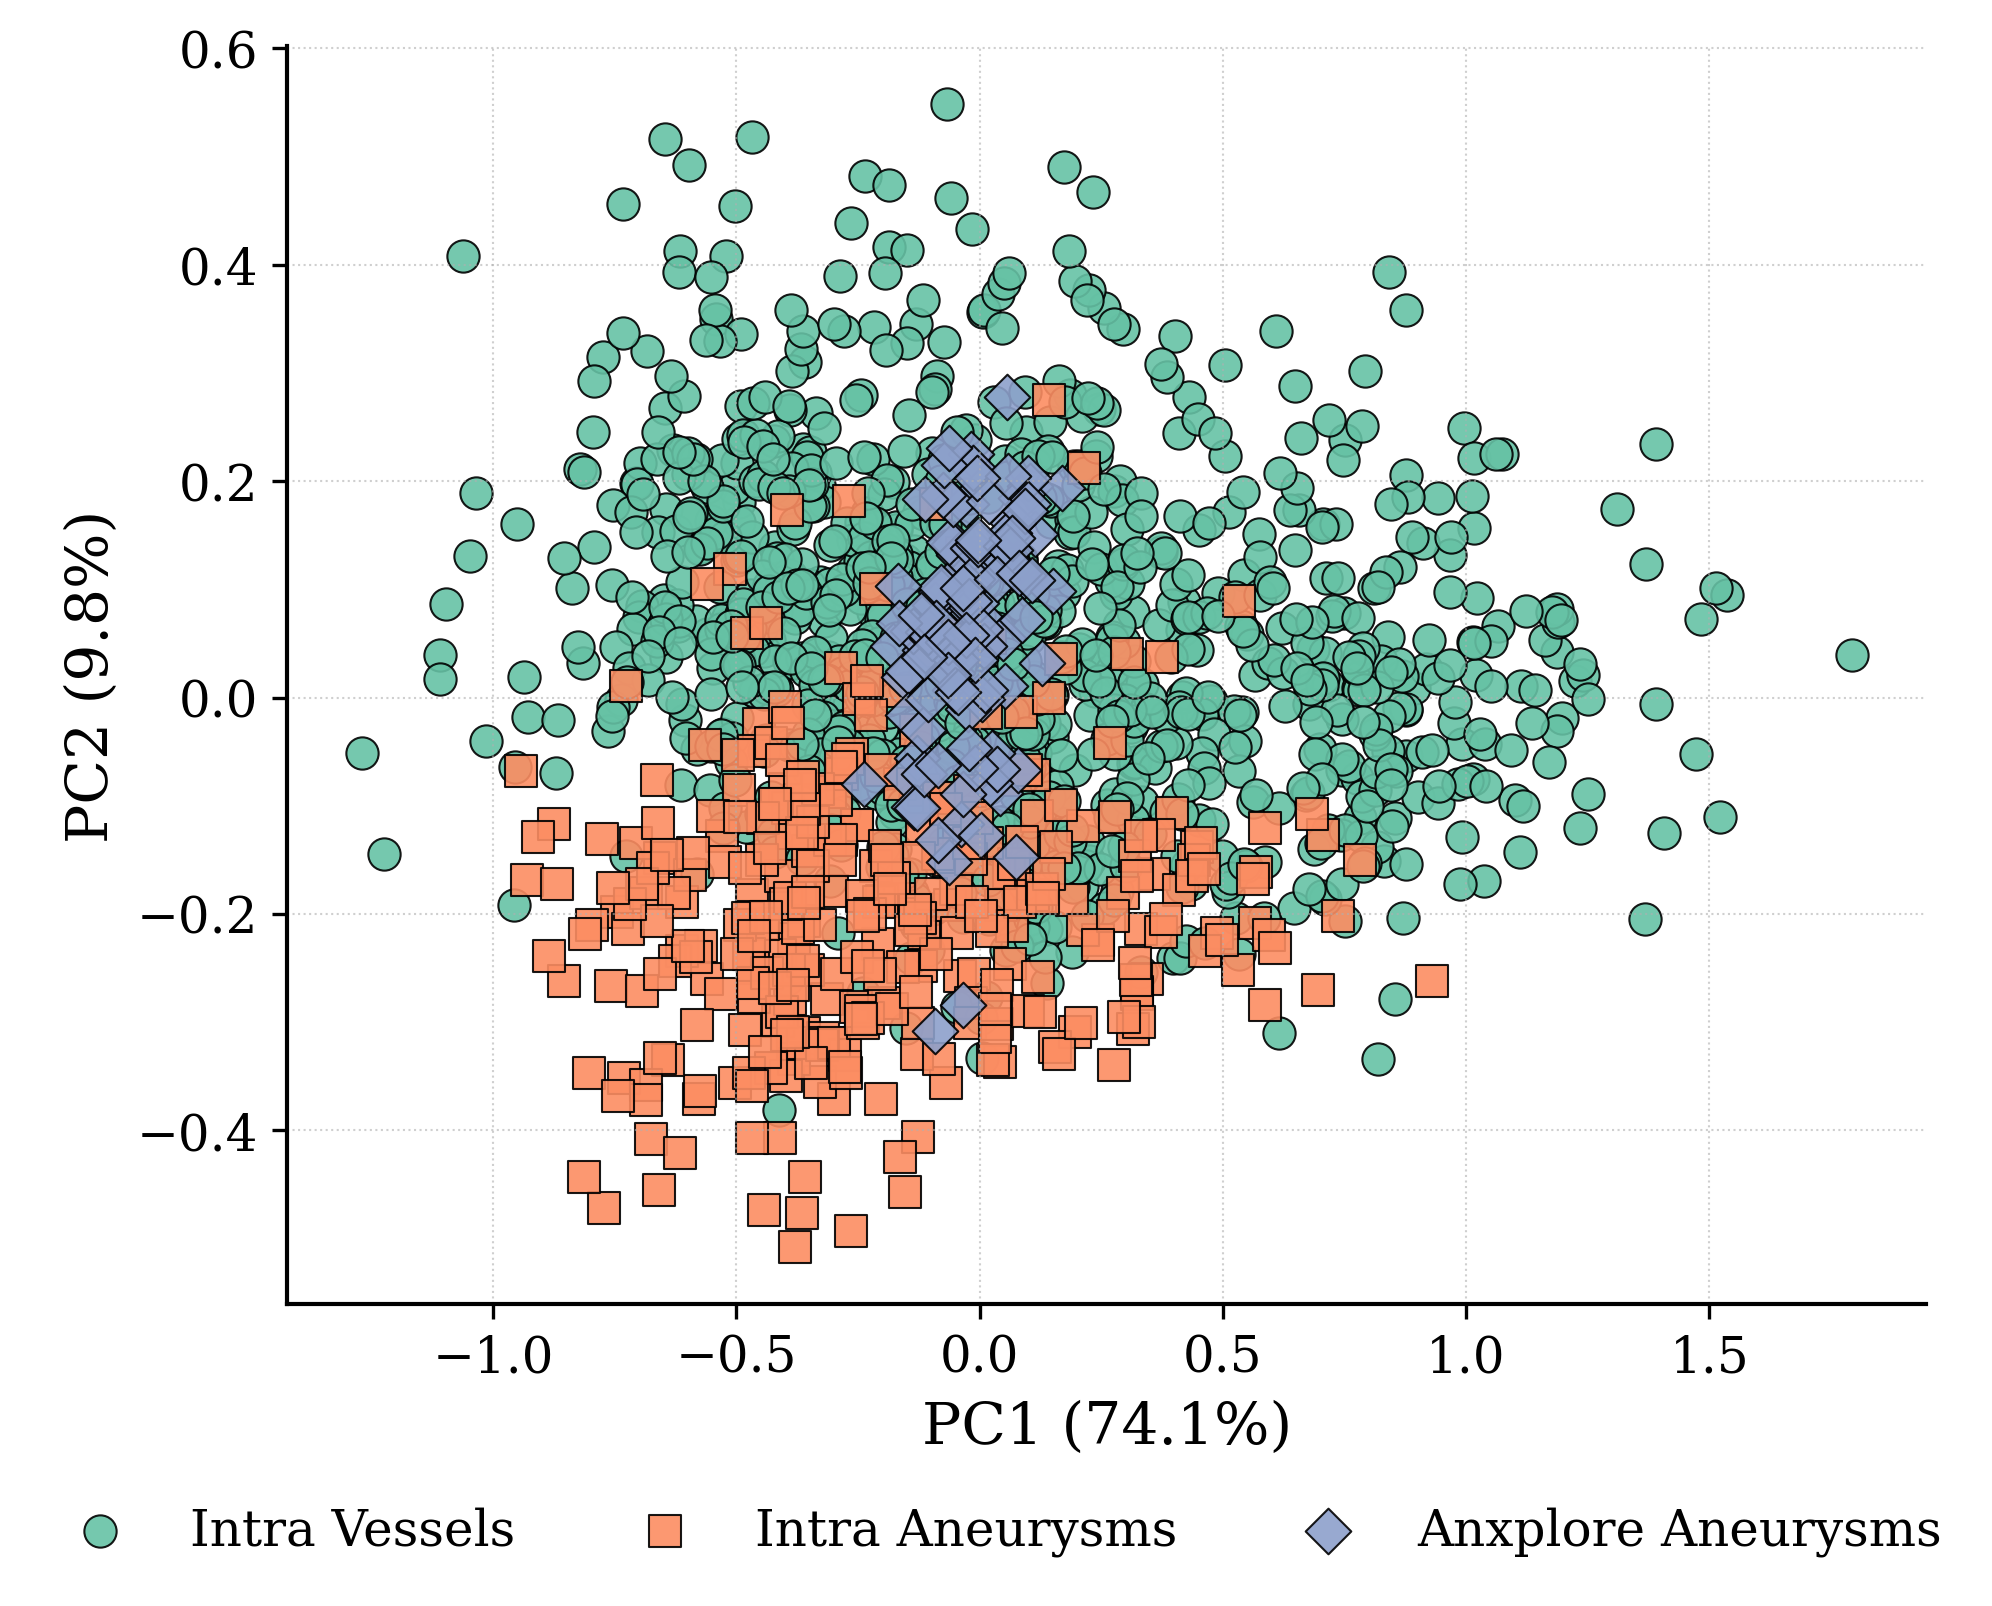
\includegraphics[width=0.33\textwidth]{pca_std.png}
  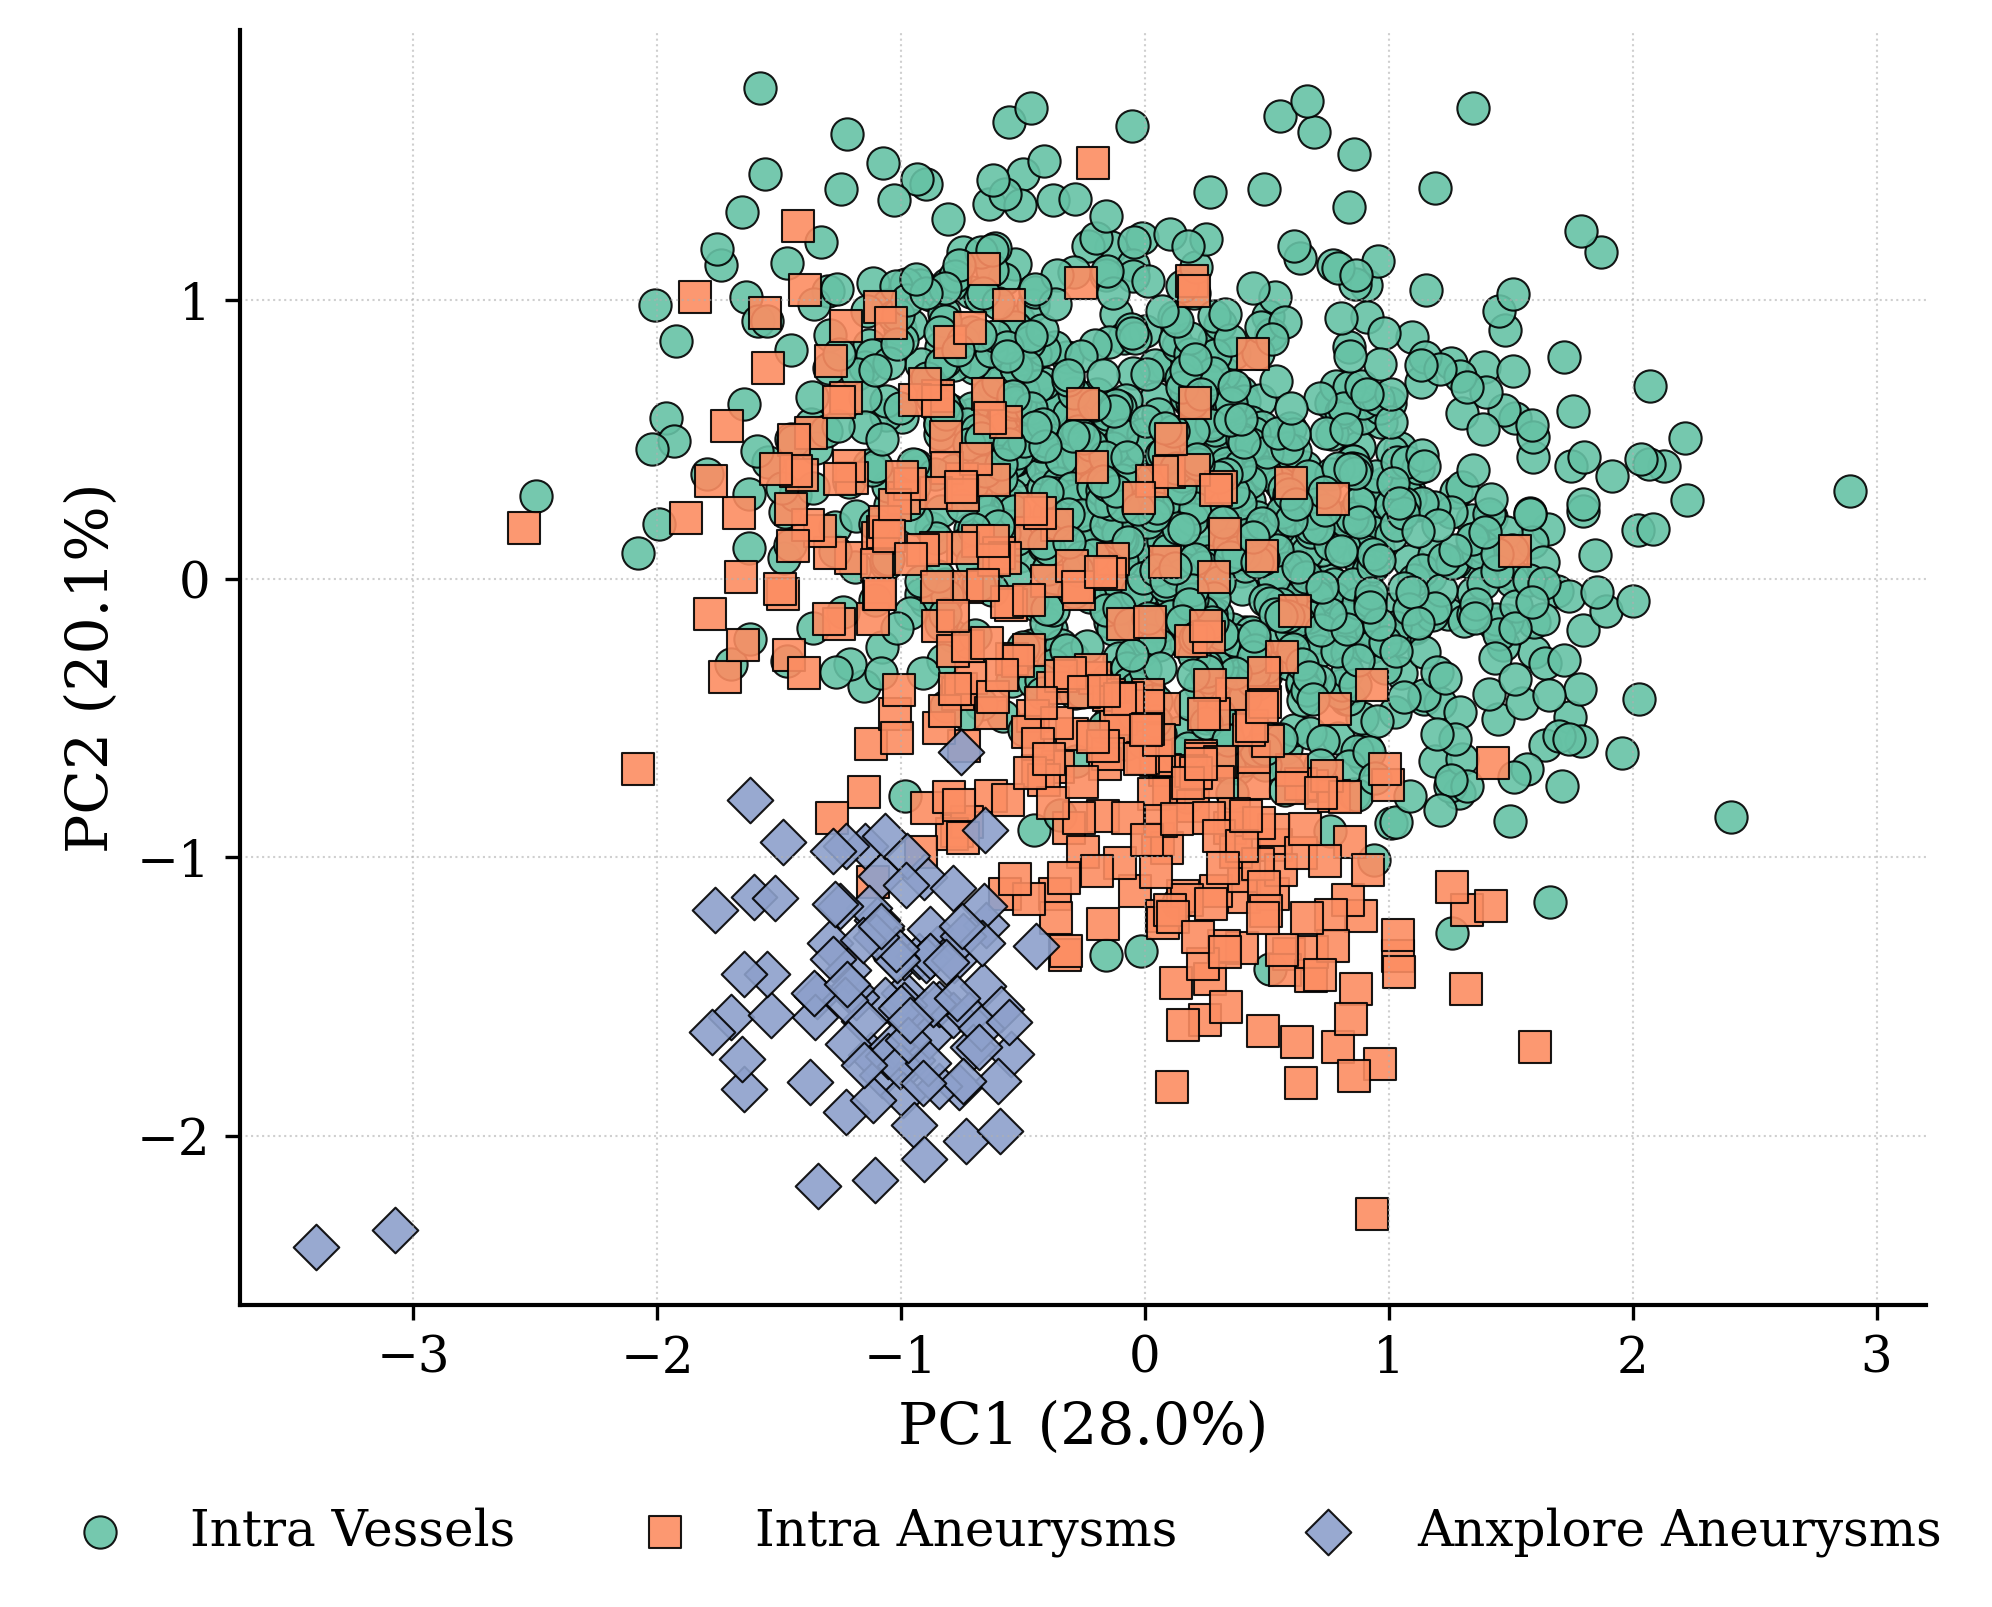
\includegraphics[width=0.33\textwidth]{pca_min.png}
  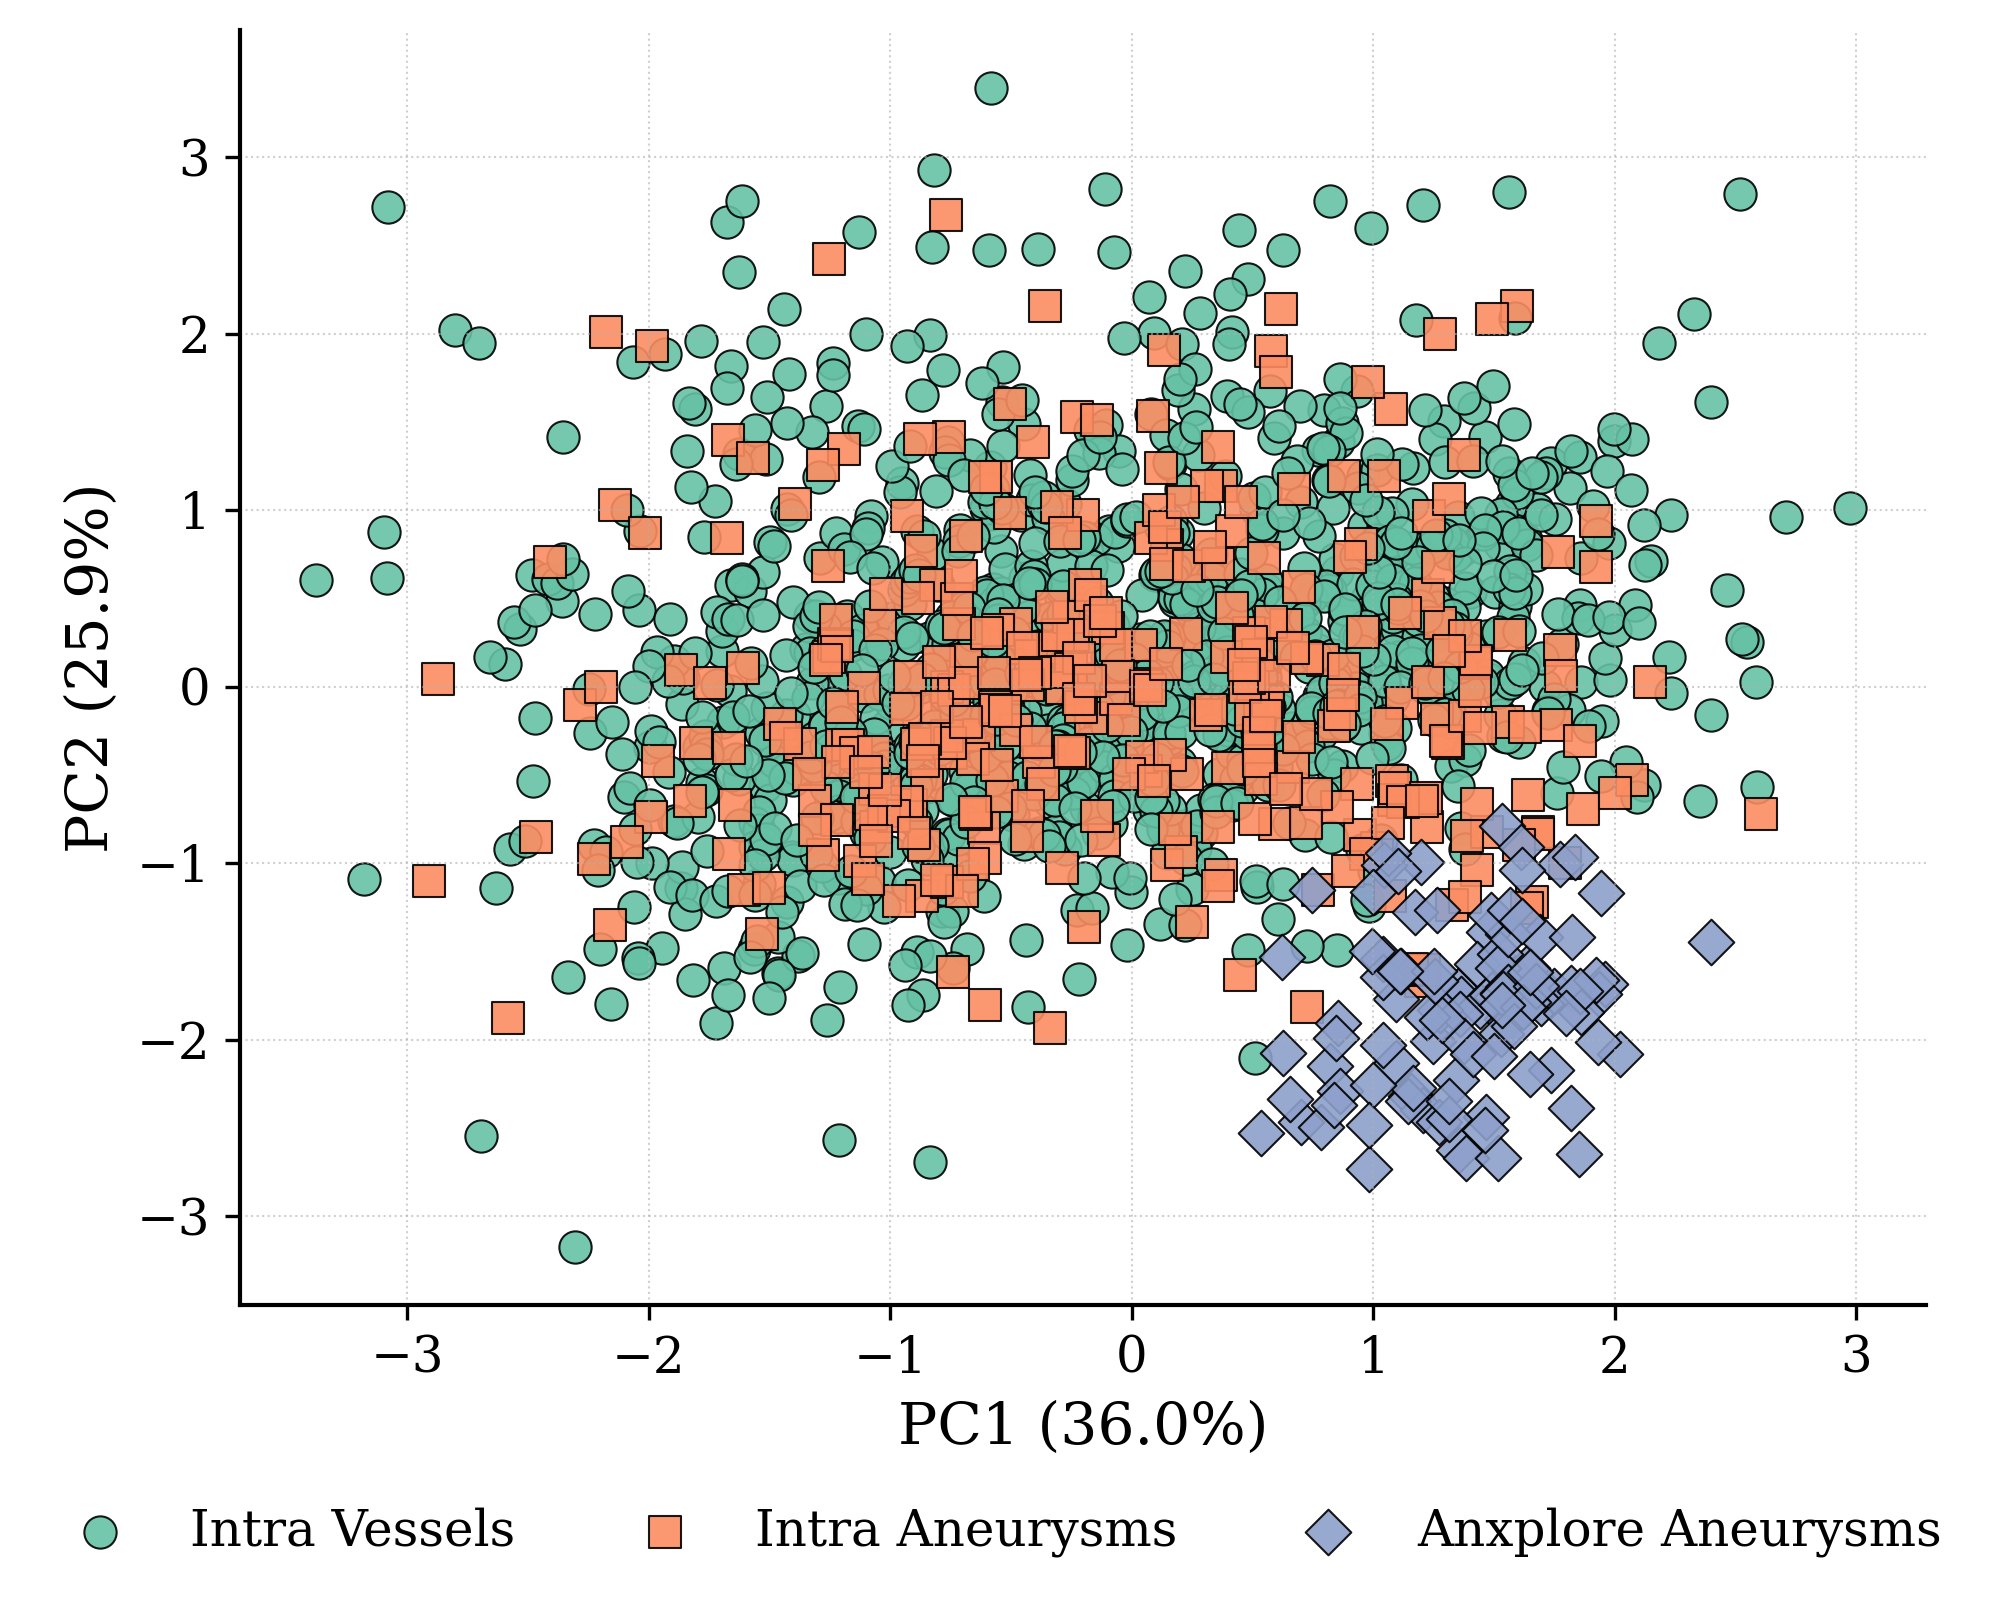
\includegraphics[width=0.33\textwidth]{pca_max.png}
  \caption{Results of PCA on the Intra 3D dataset combined with the AnXplore dataset. Figures show the mean, standard deviation, minimum, and maximum of the PCA components.}
  \label{fig:pca_supplementary_all}
\end{figure}

\vspace{-0.55cm}

\begin{figure}[h!]
    \centering
    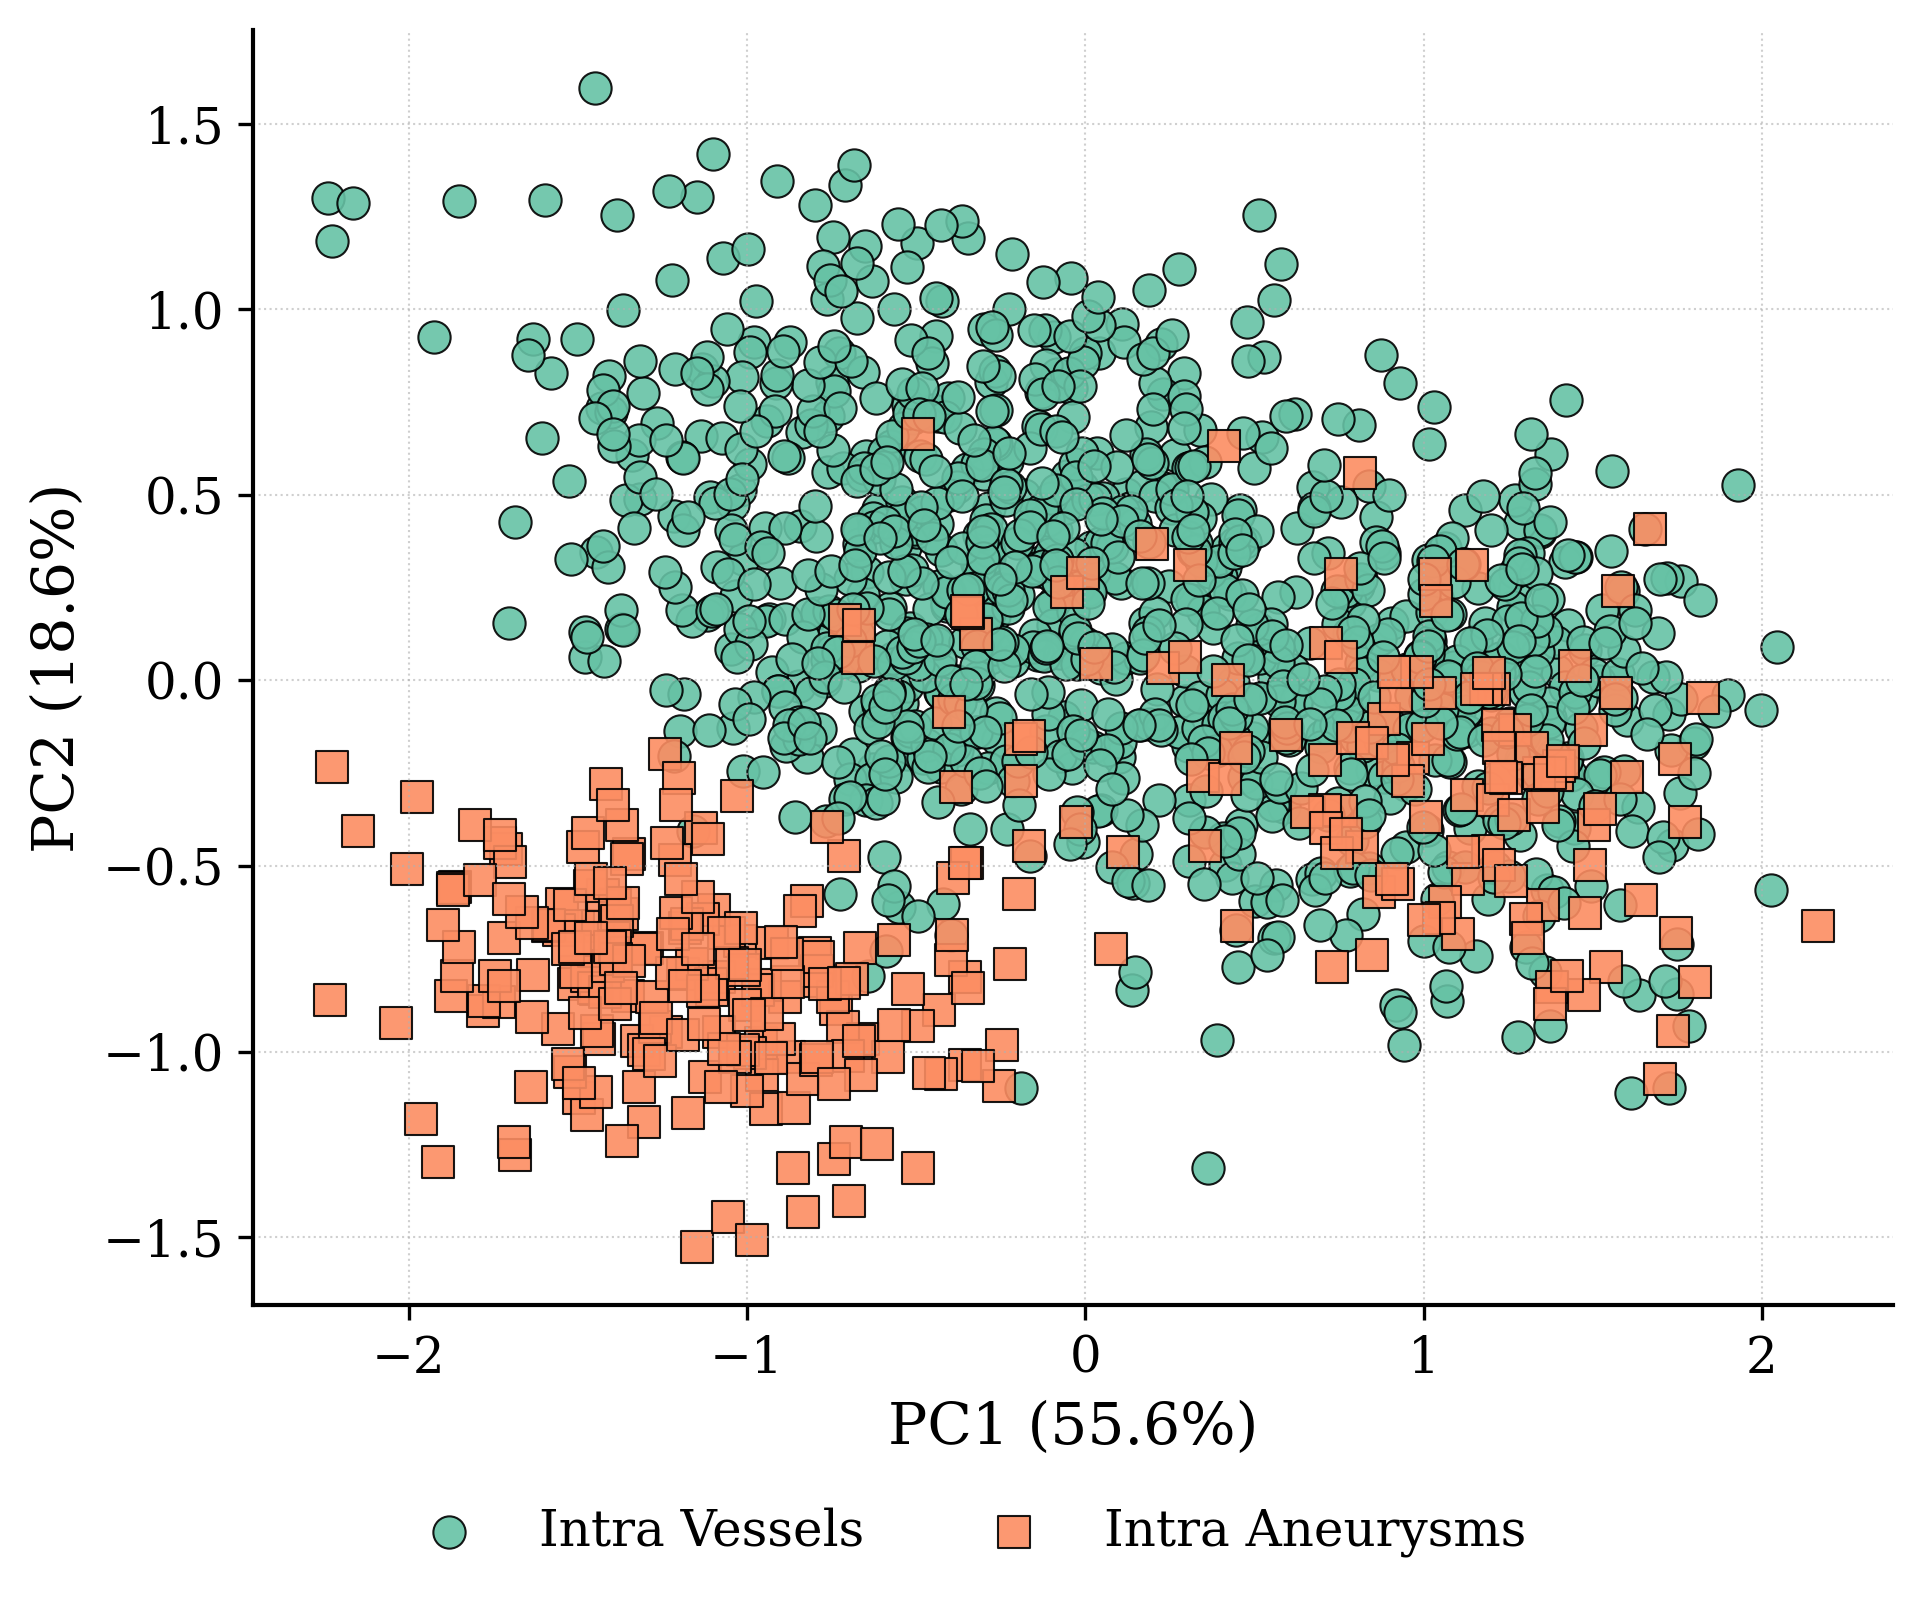
\includegraphics[width=0.33\textwidth]{pca_intra_mean.png}
    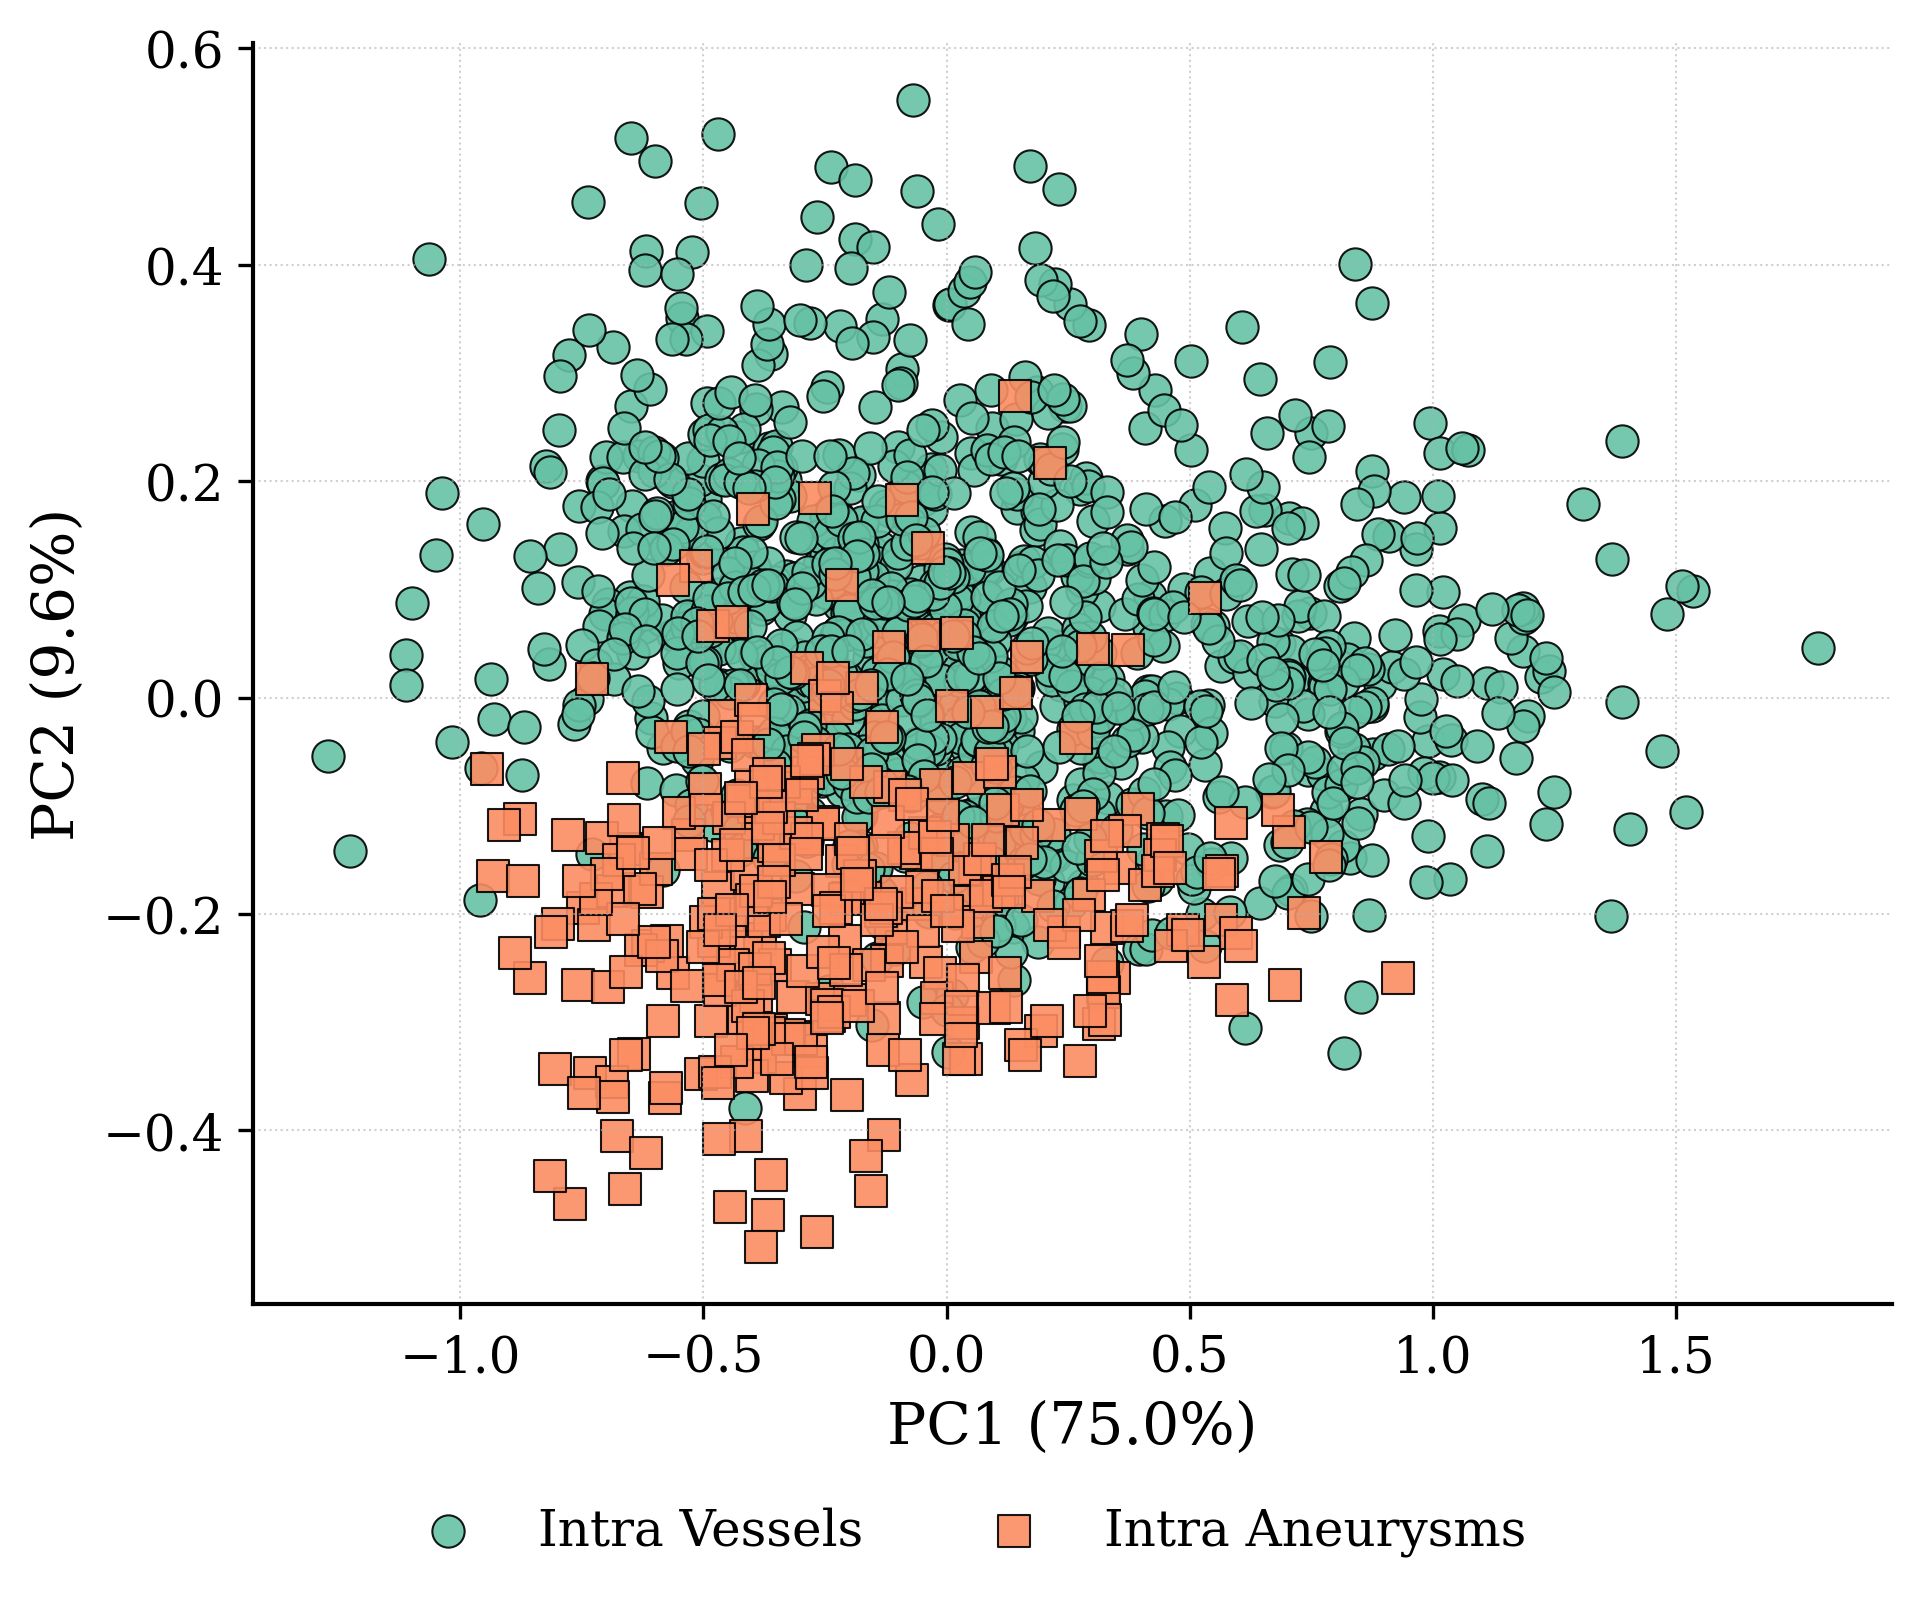
\includegraphics[width=0.33\textwidth]{pca_intra_std.png}
    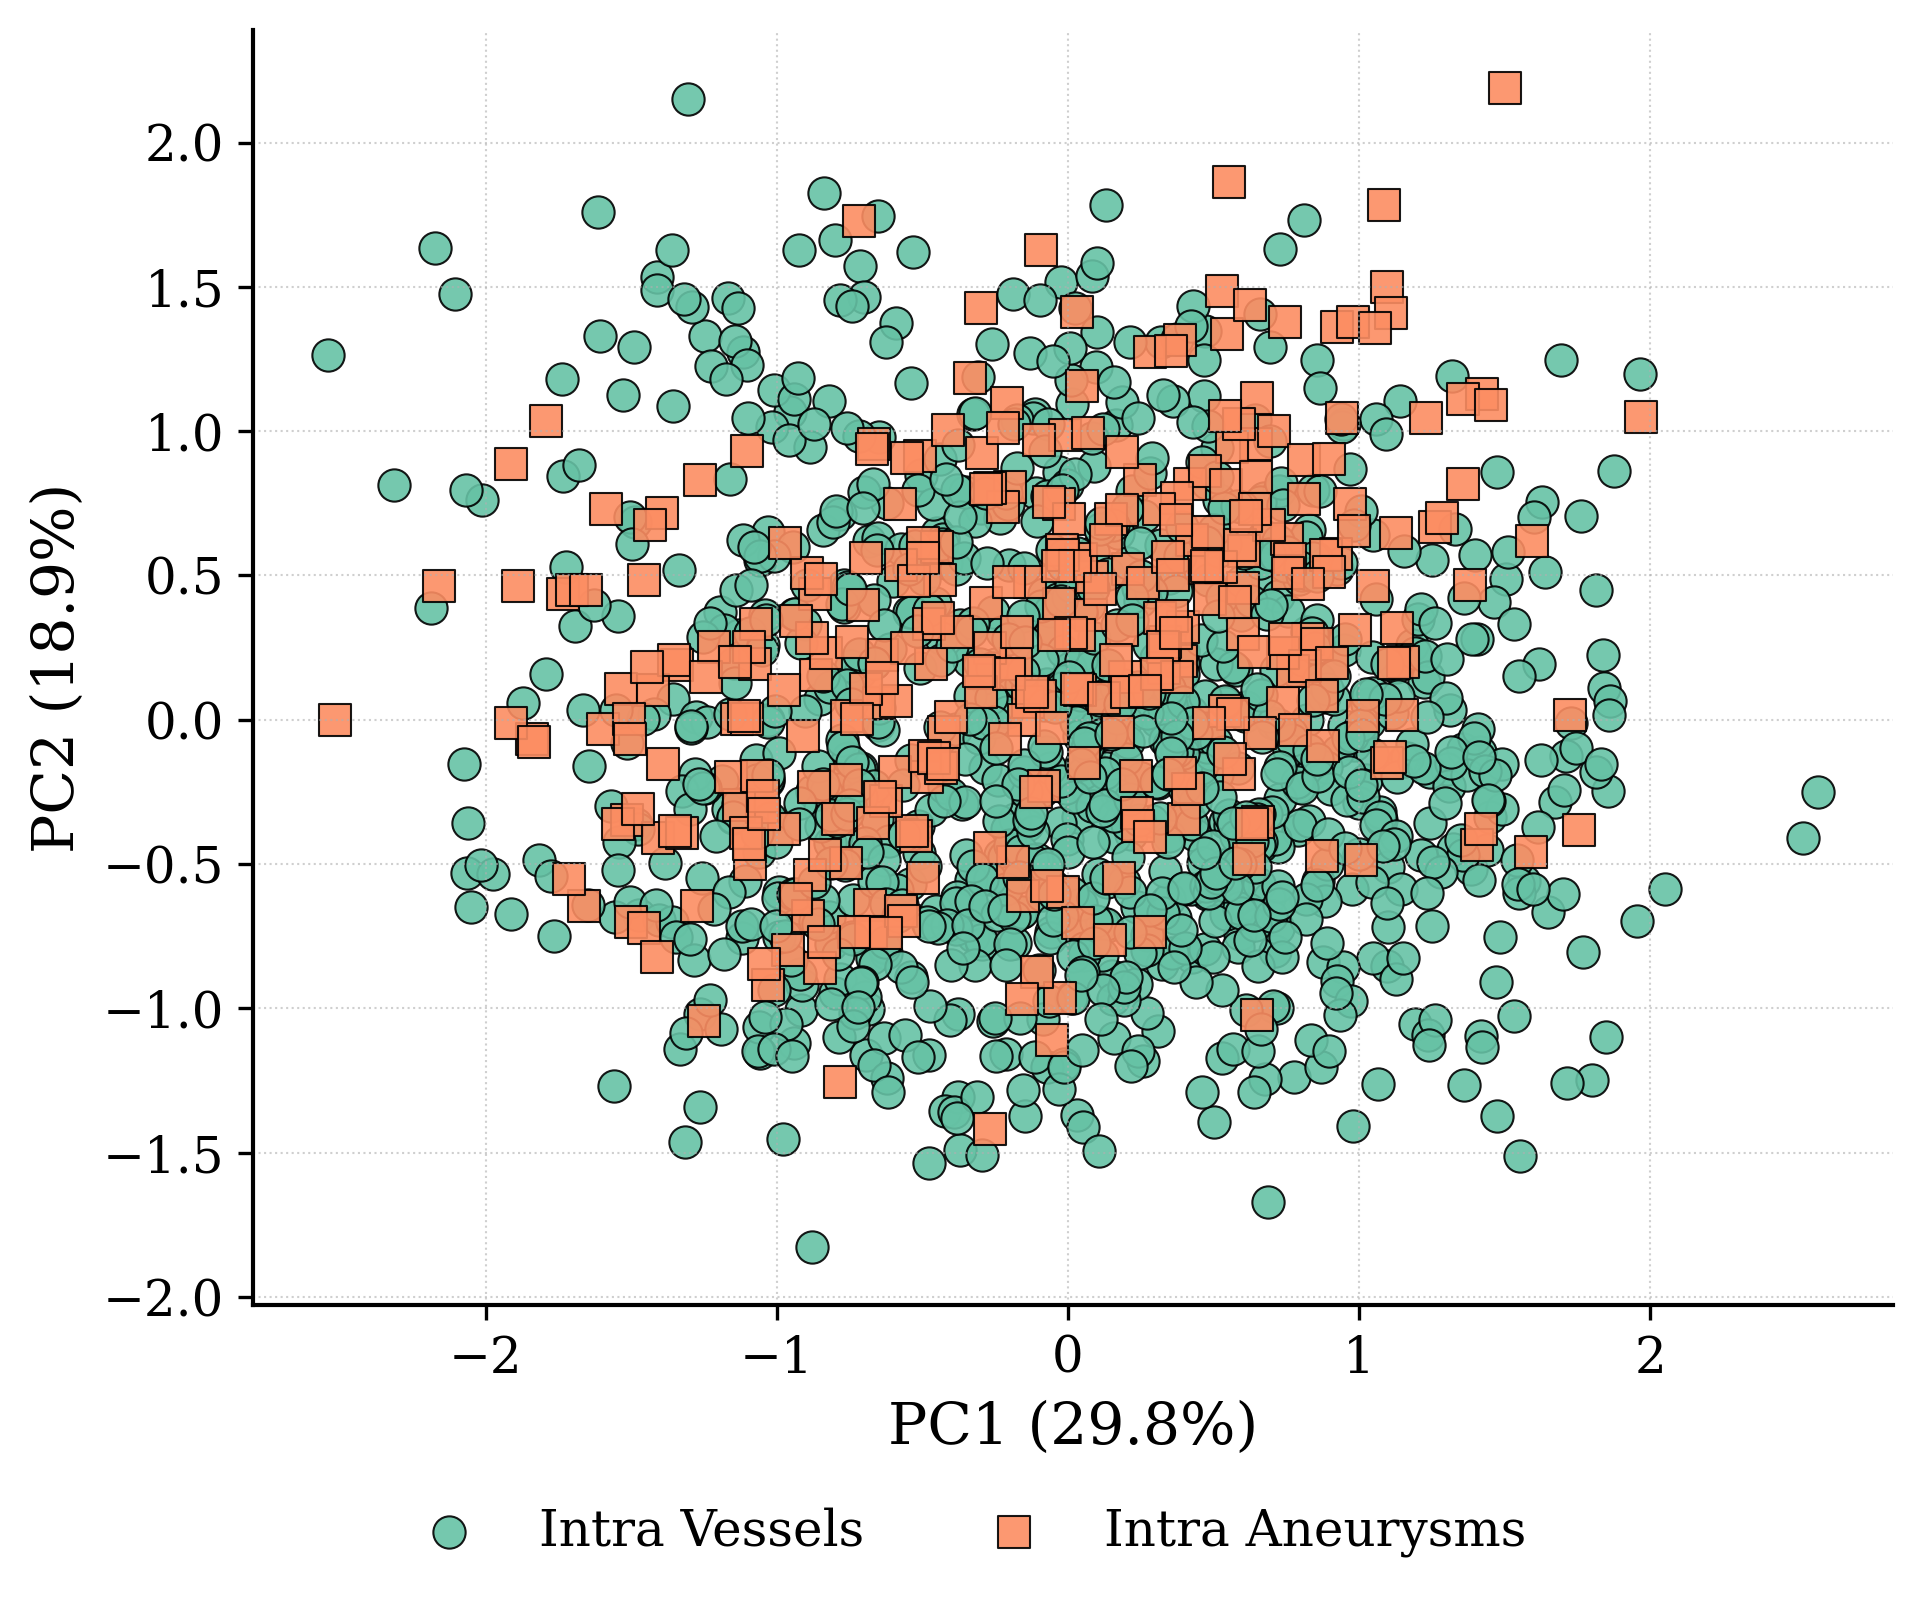
\includegraphics[width=0.33\textwidth]{pca_intra_min.png}
    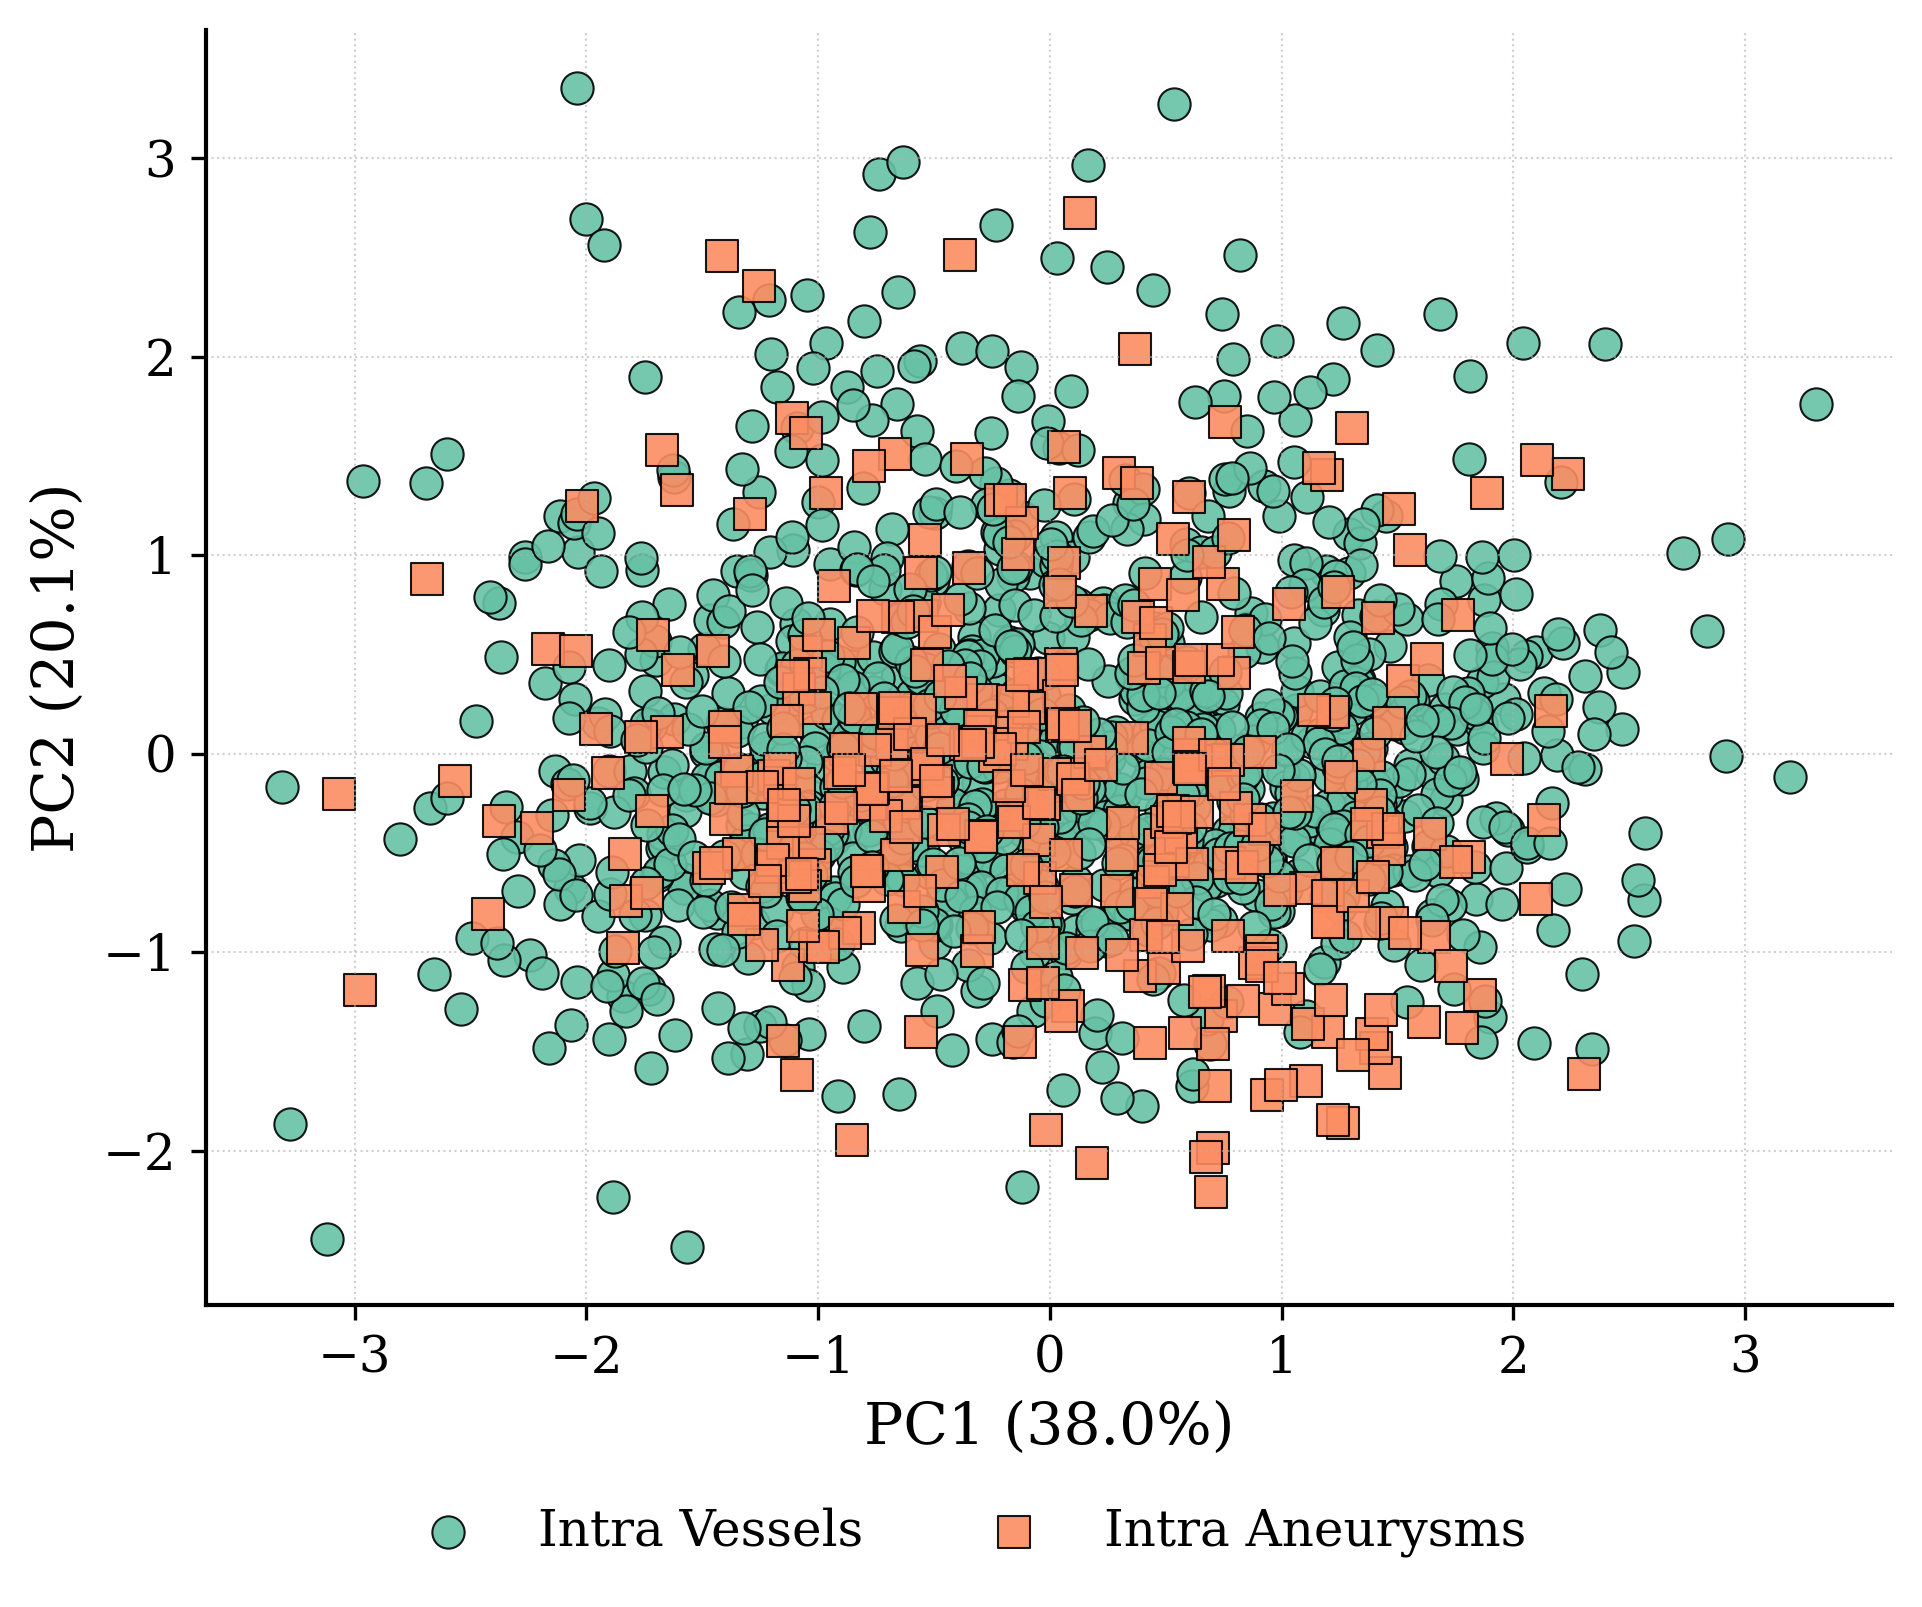
\includegraphics[width=0.33\textwidth]{pca_intra_max.png}
    \caption{Results of PCA on the Intra 3D dataset. Figures show the mean, standard deviation, minimum, and maximum of the PCA components.}
    \label{fig:pca_supplementary_intra}
\end{figure}

\begin{figure}[h!]
  \centering
  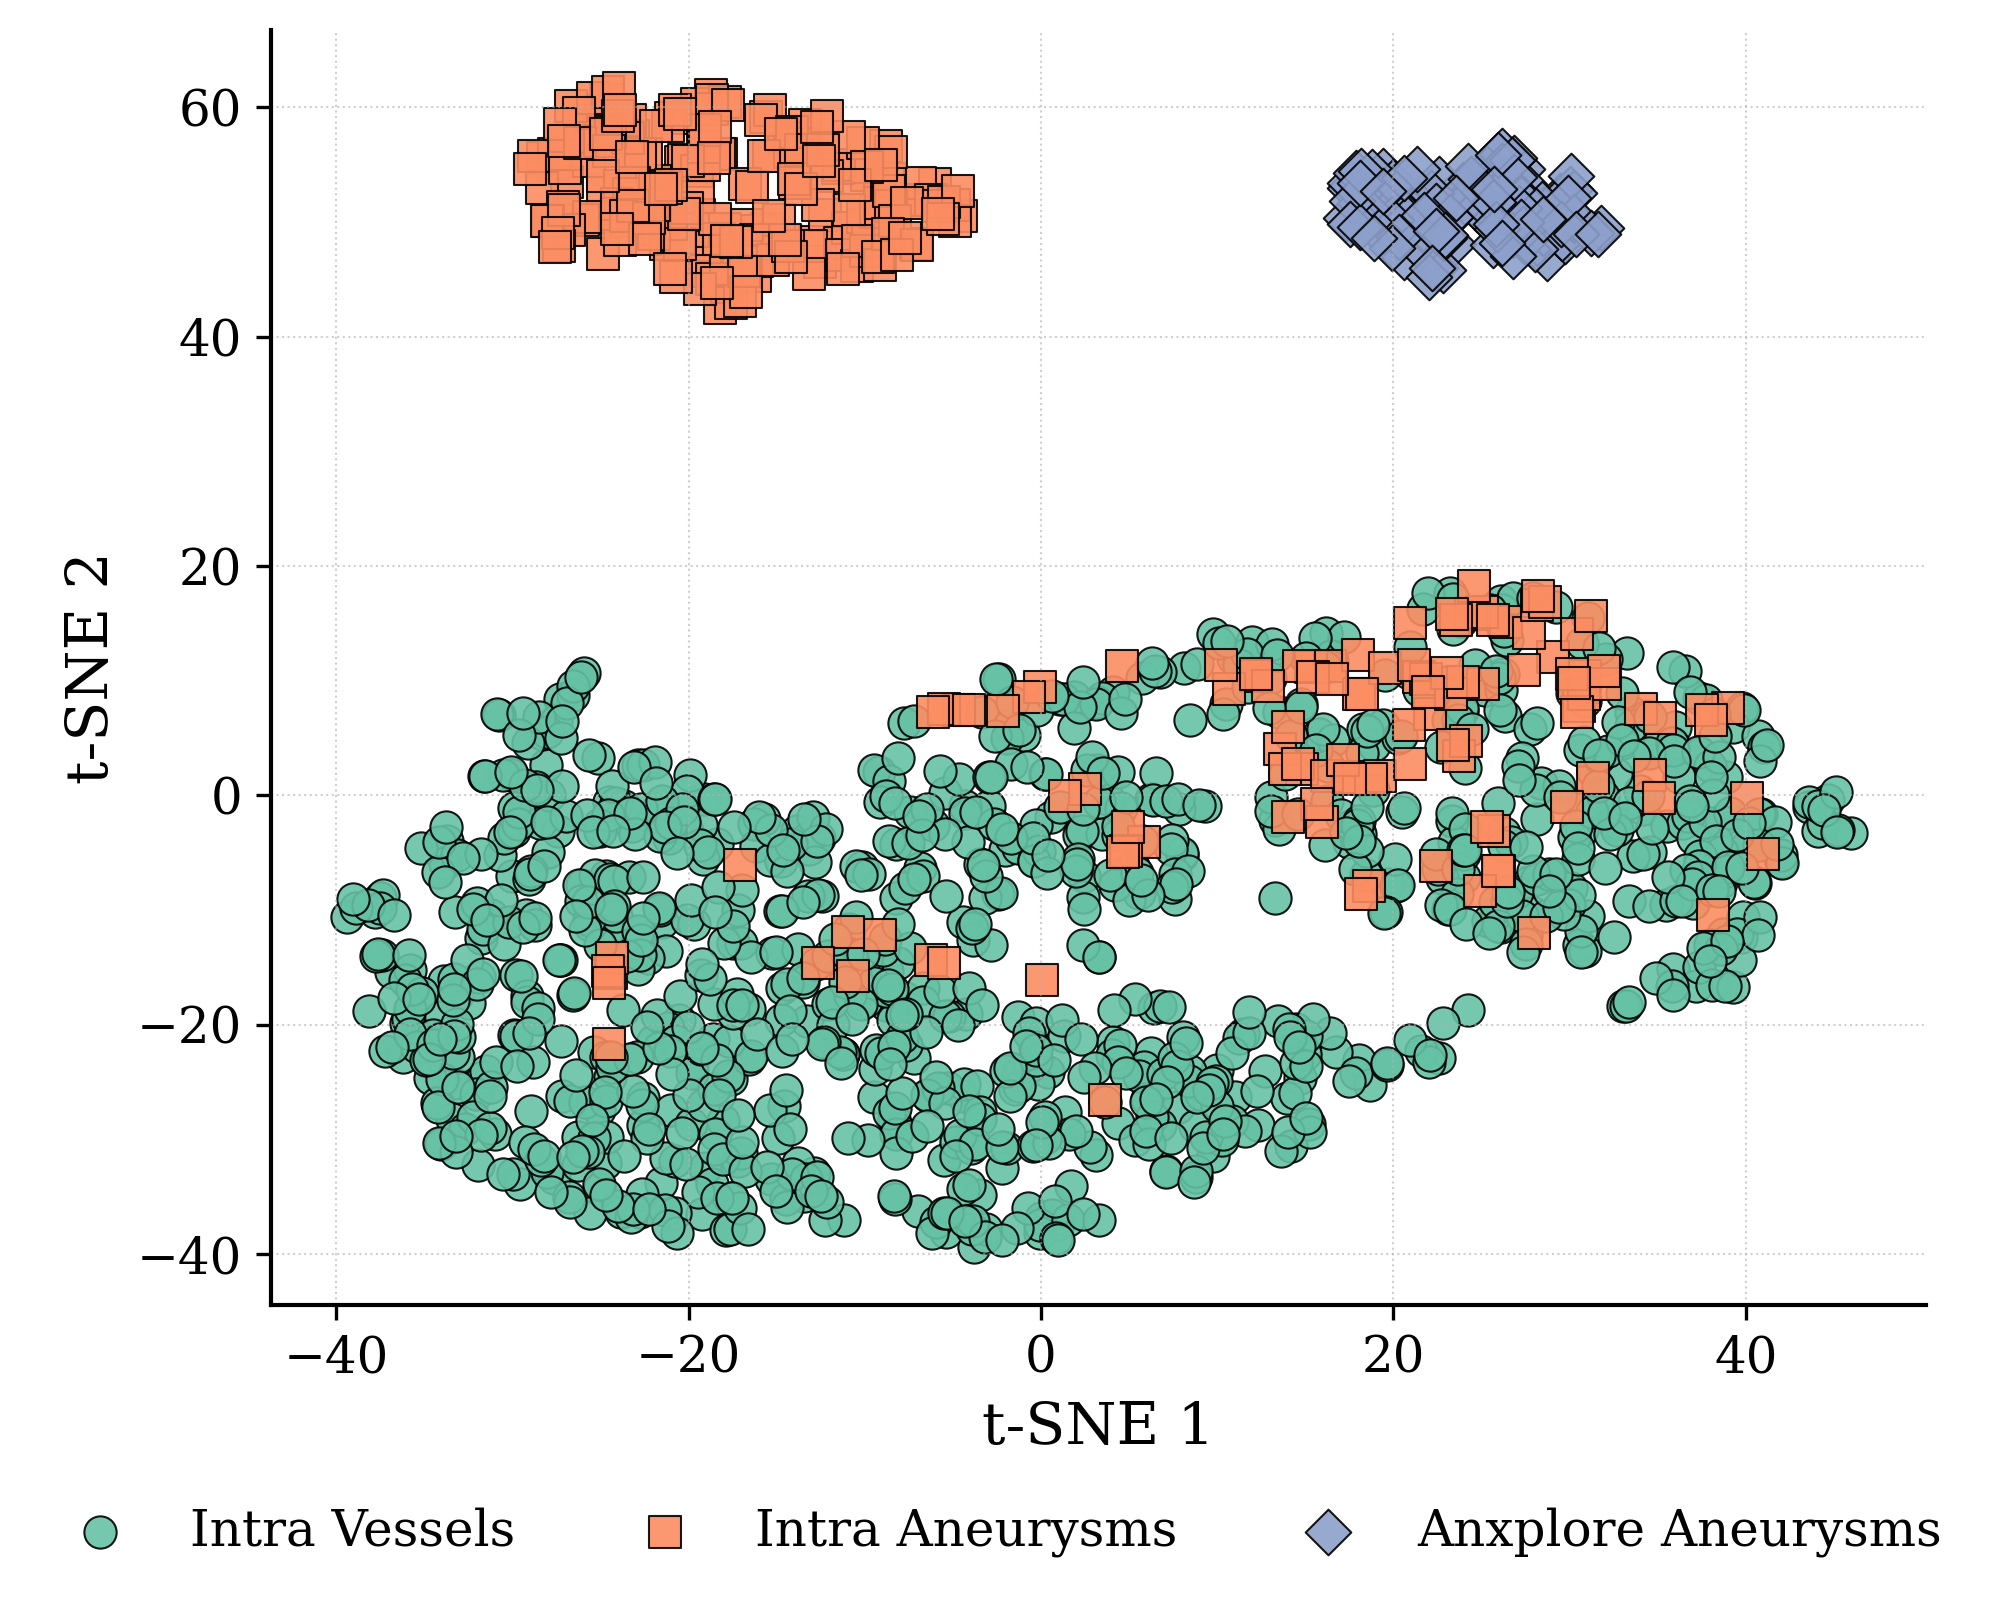
\includegraphics[width=0.34\textwidth]{t-sne_mean.png}
  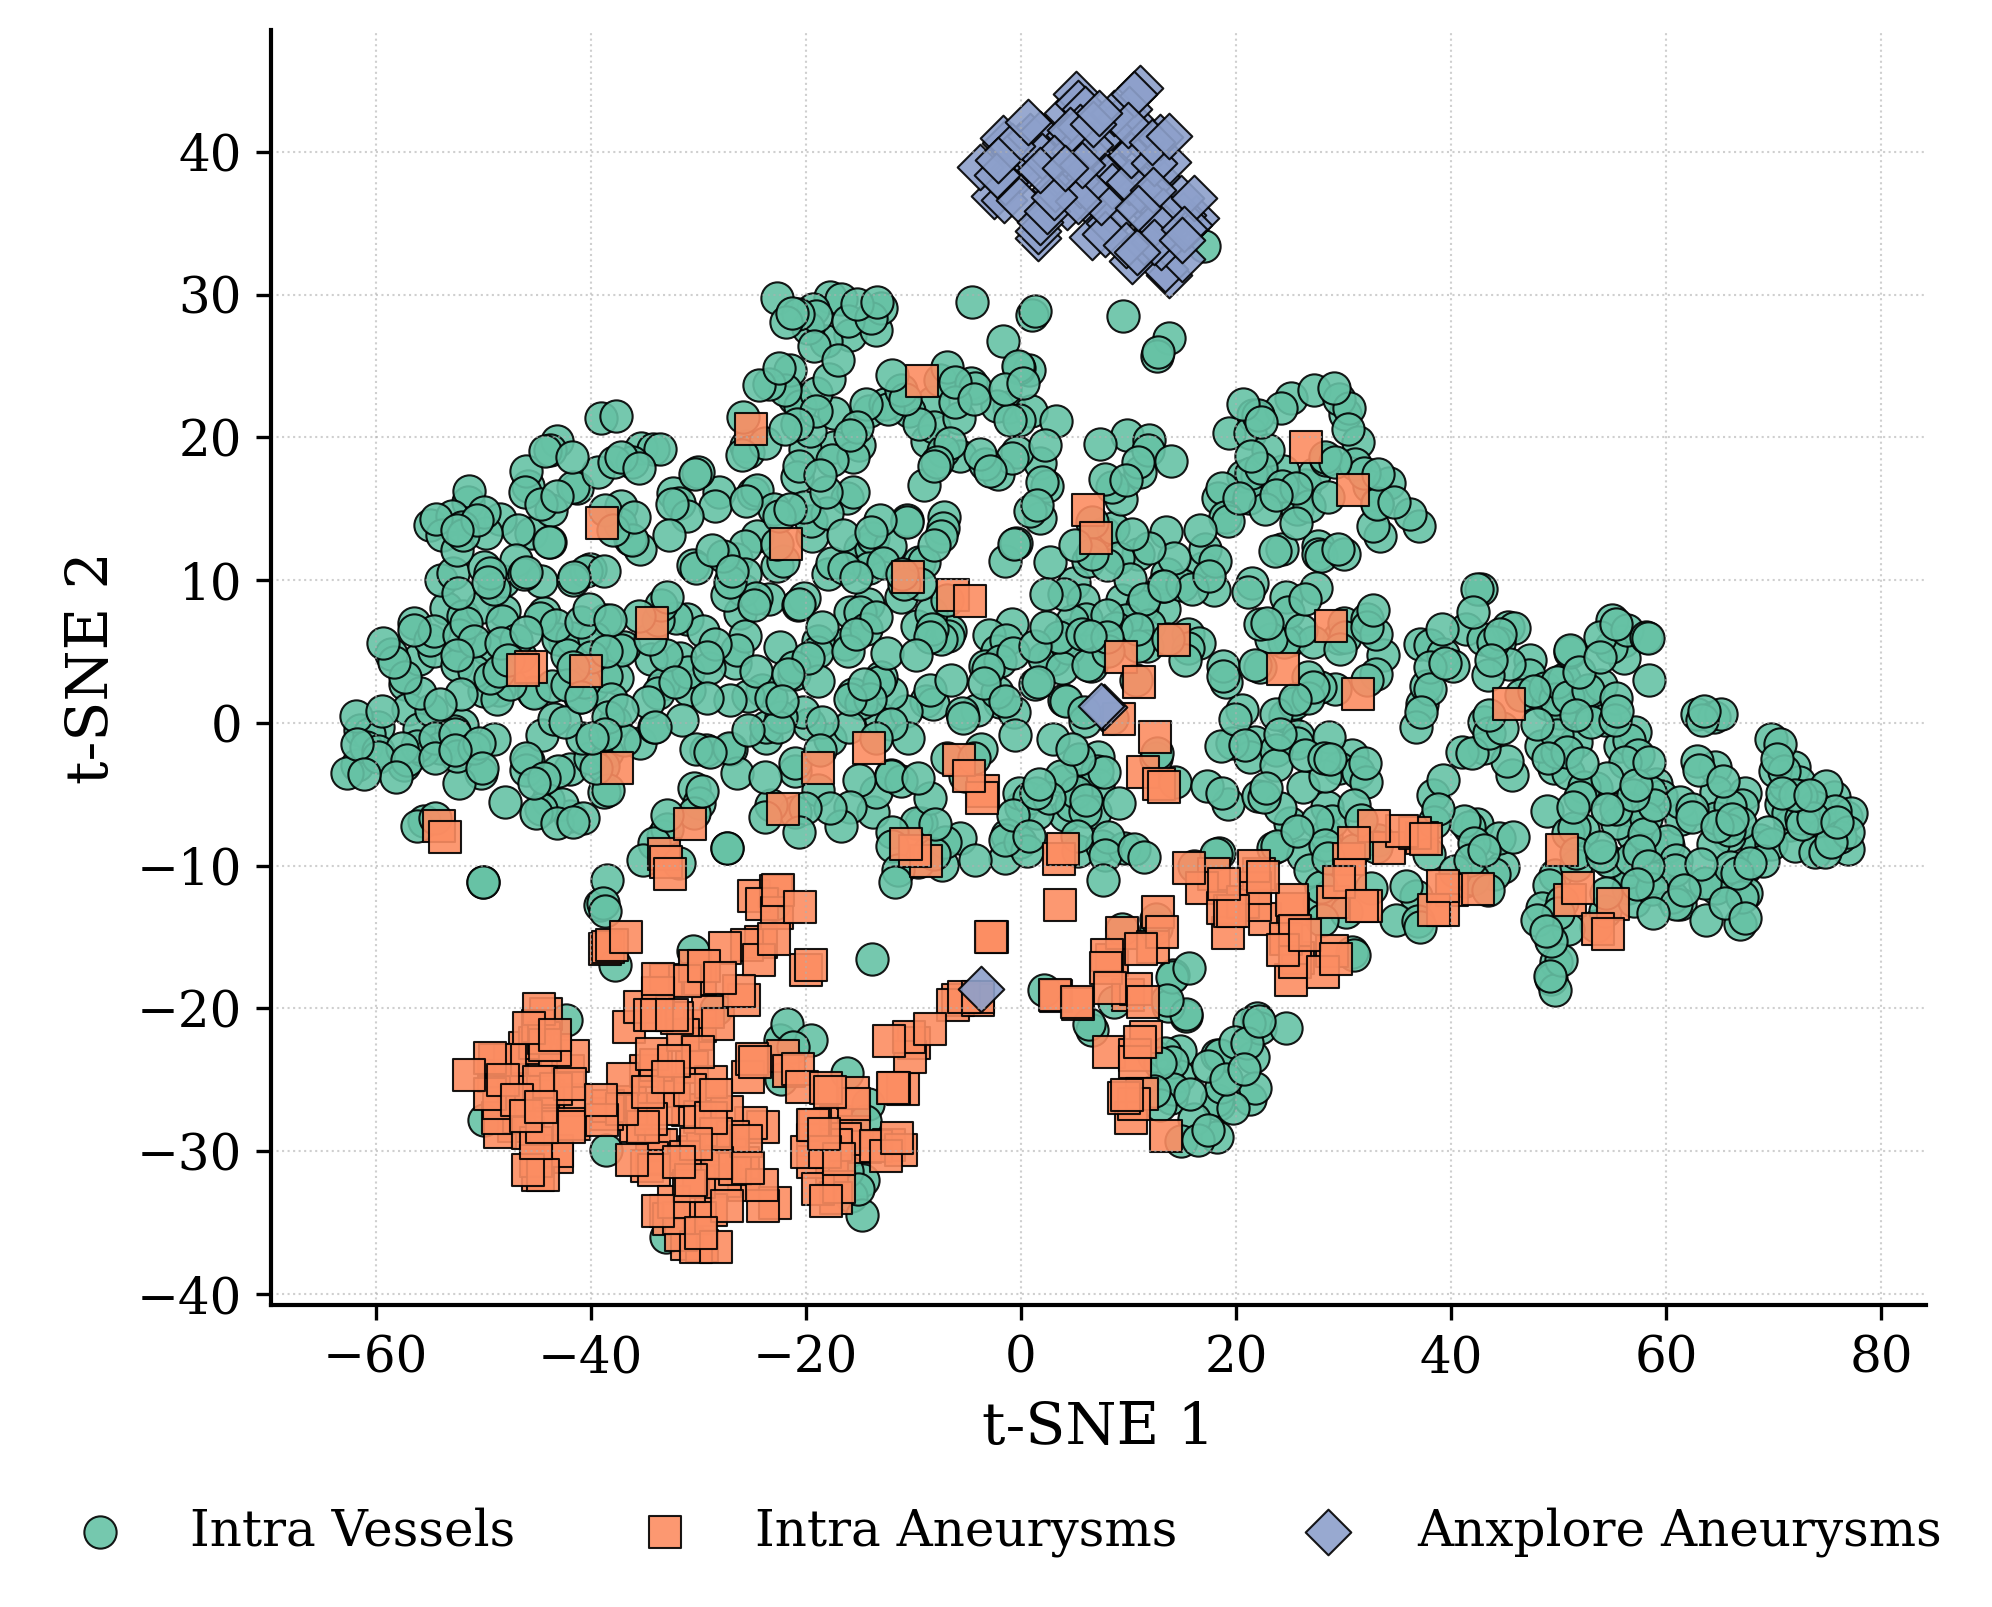
\includegraphics[width=0.34\textwidth]{t-sne_std.png}
  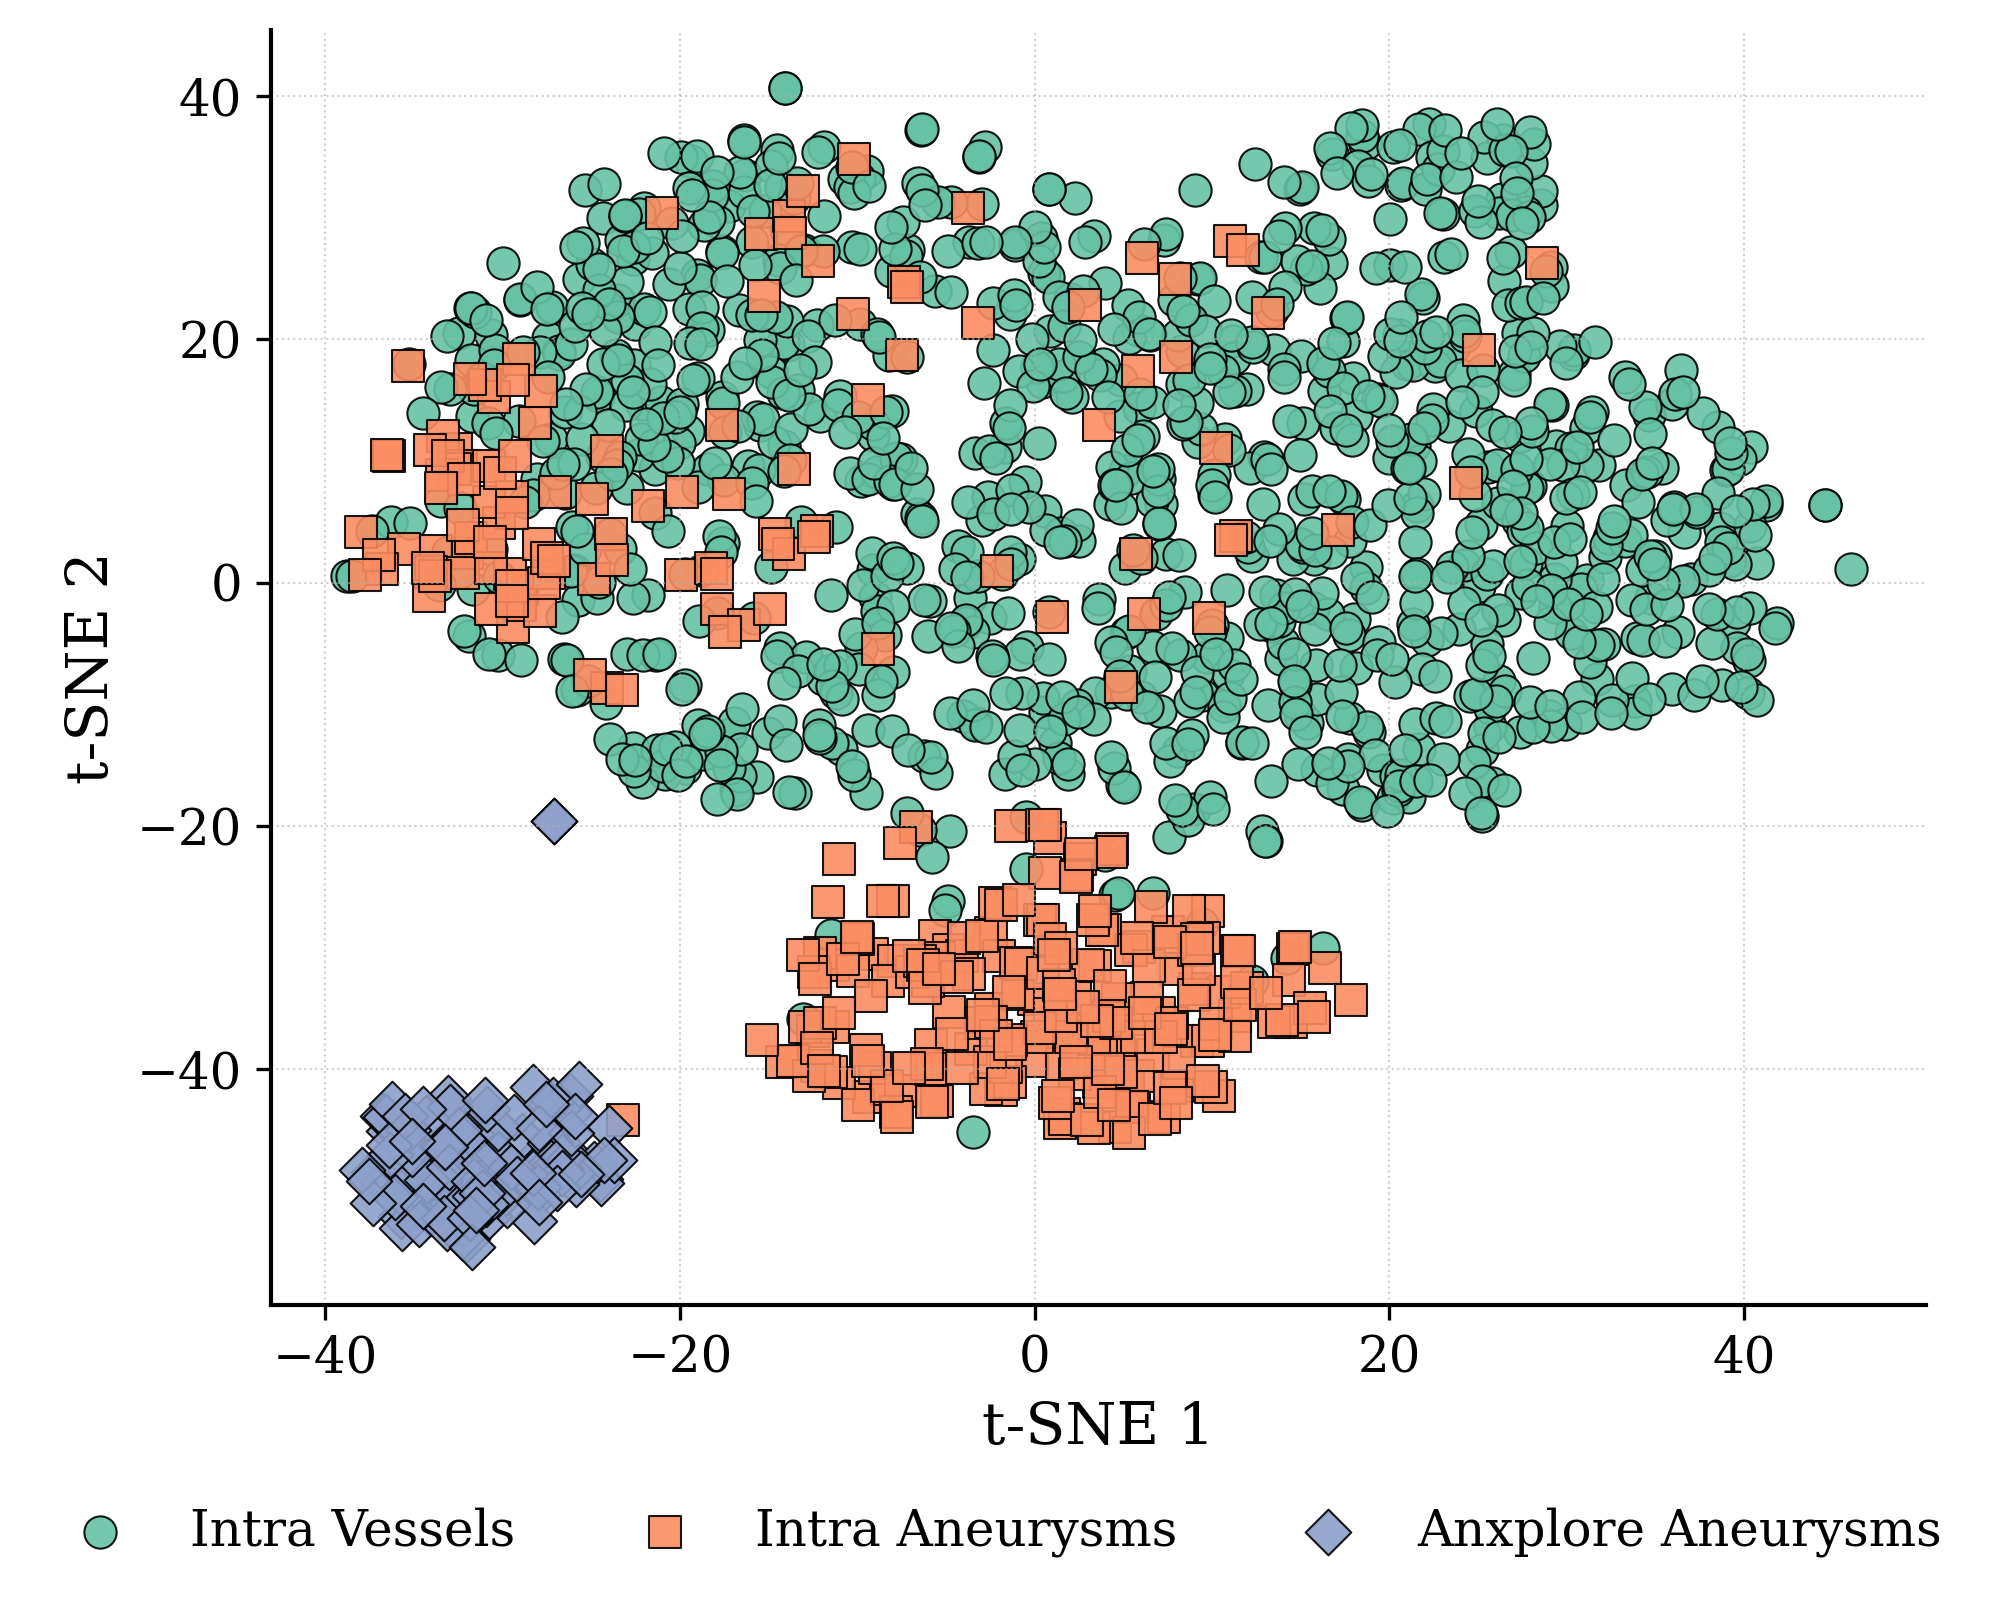
\includegraphics[width=0.34\textwidth]{t-sne_min.png}
  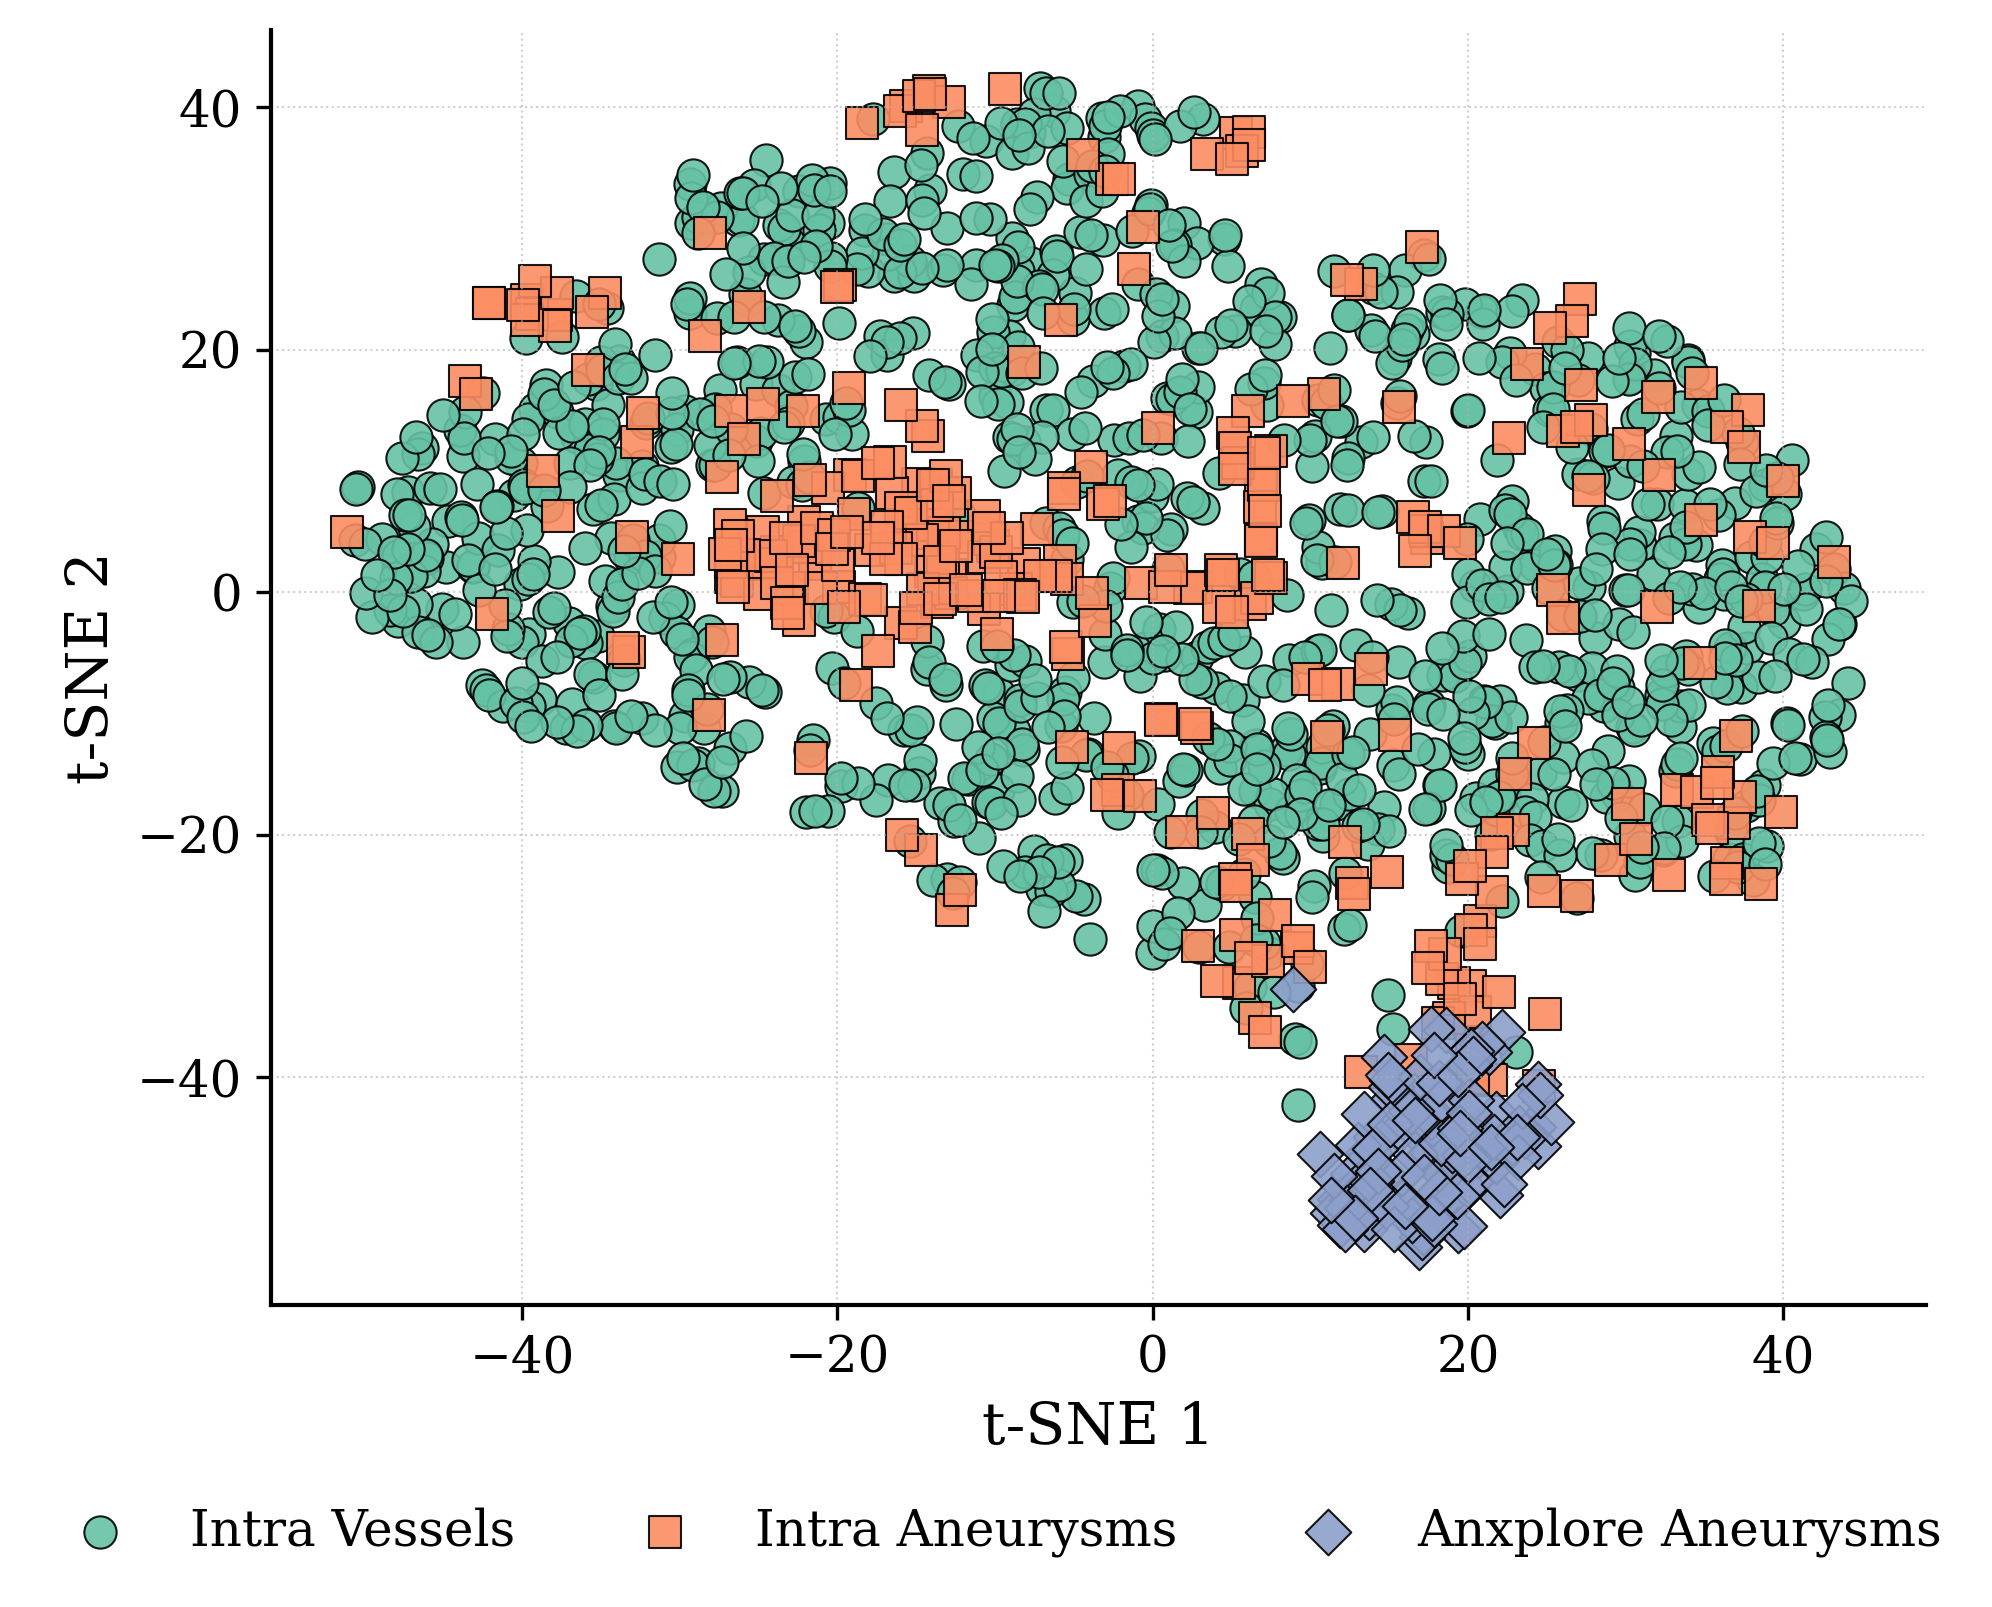
\includegraphics[width=0.34\textwidth]{t-sne_max.png}
  \caption{Result of t-SNE on the Intra 3D dataset combined with the AnXplore dataset. Figures show the mean, standard deviation, minimum, and maximum of the t-SNE components.}
  \label{fig:tsne_supplementary}
\end{figure}

\begin{figure}[h]
  \centering
  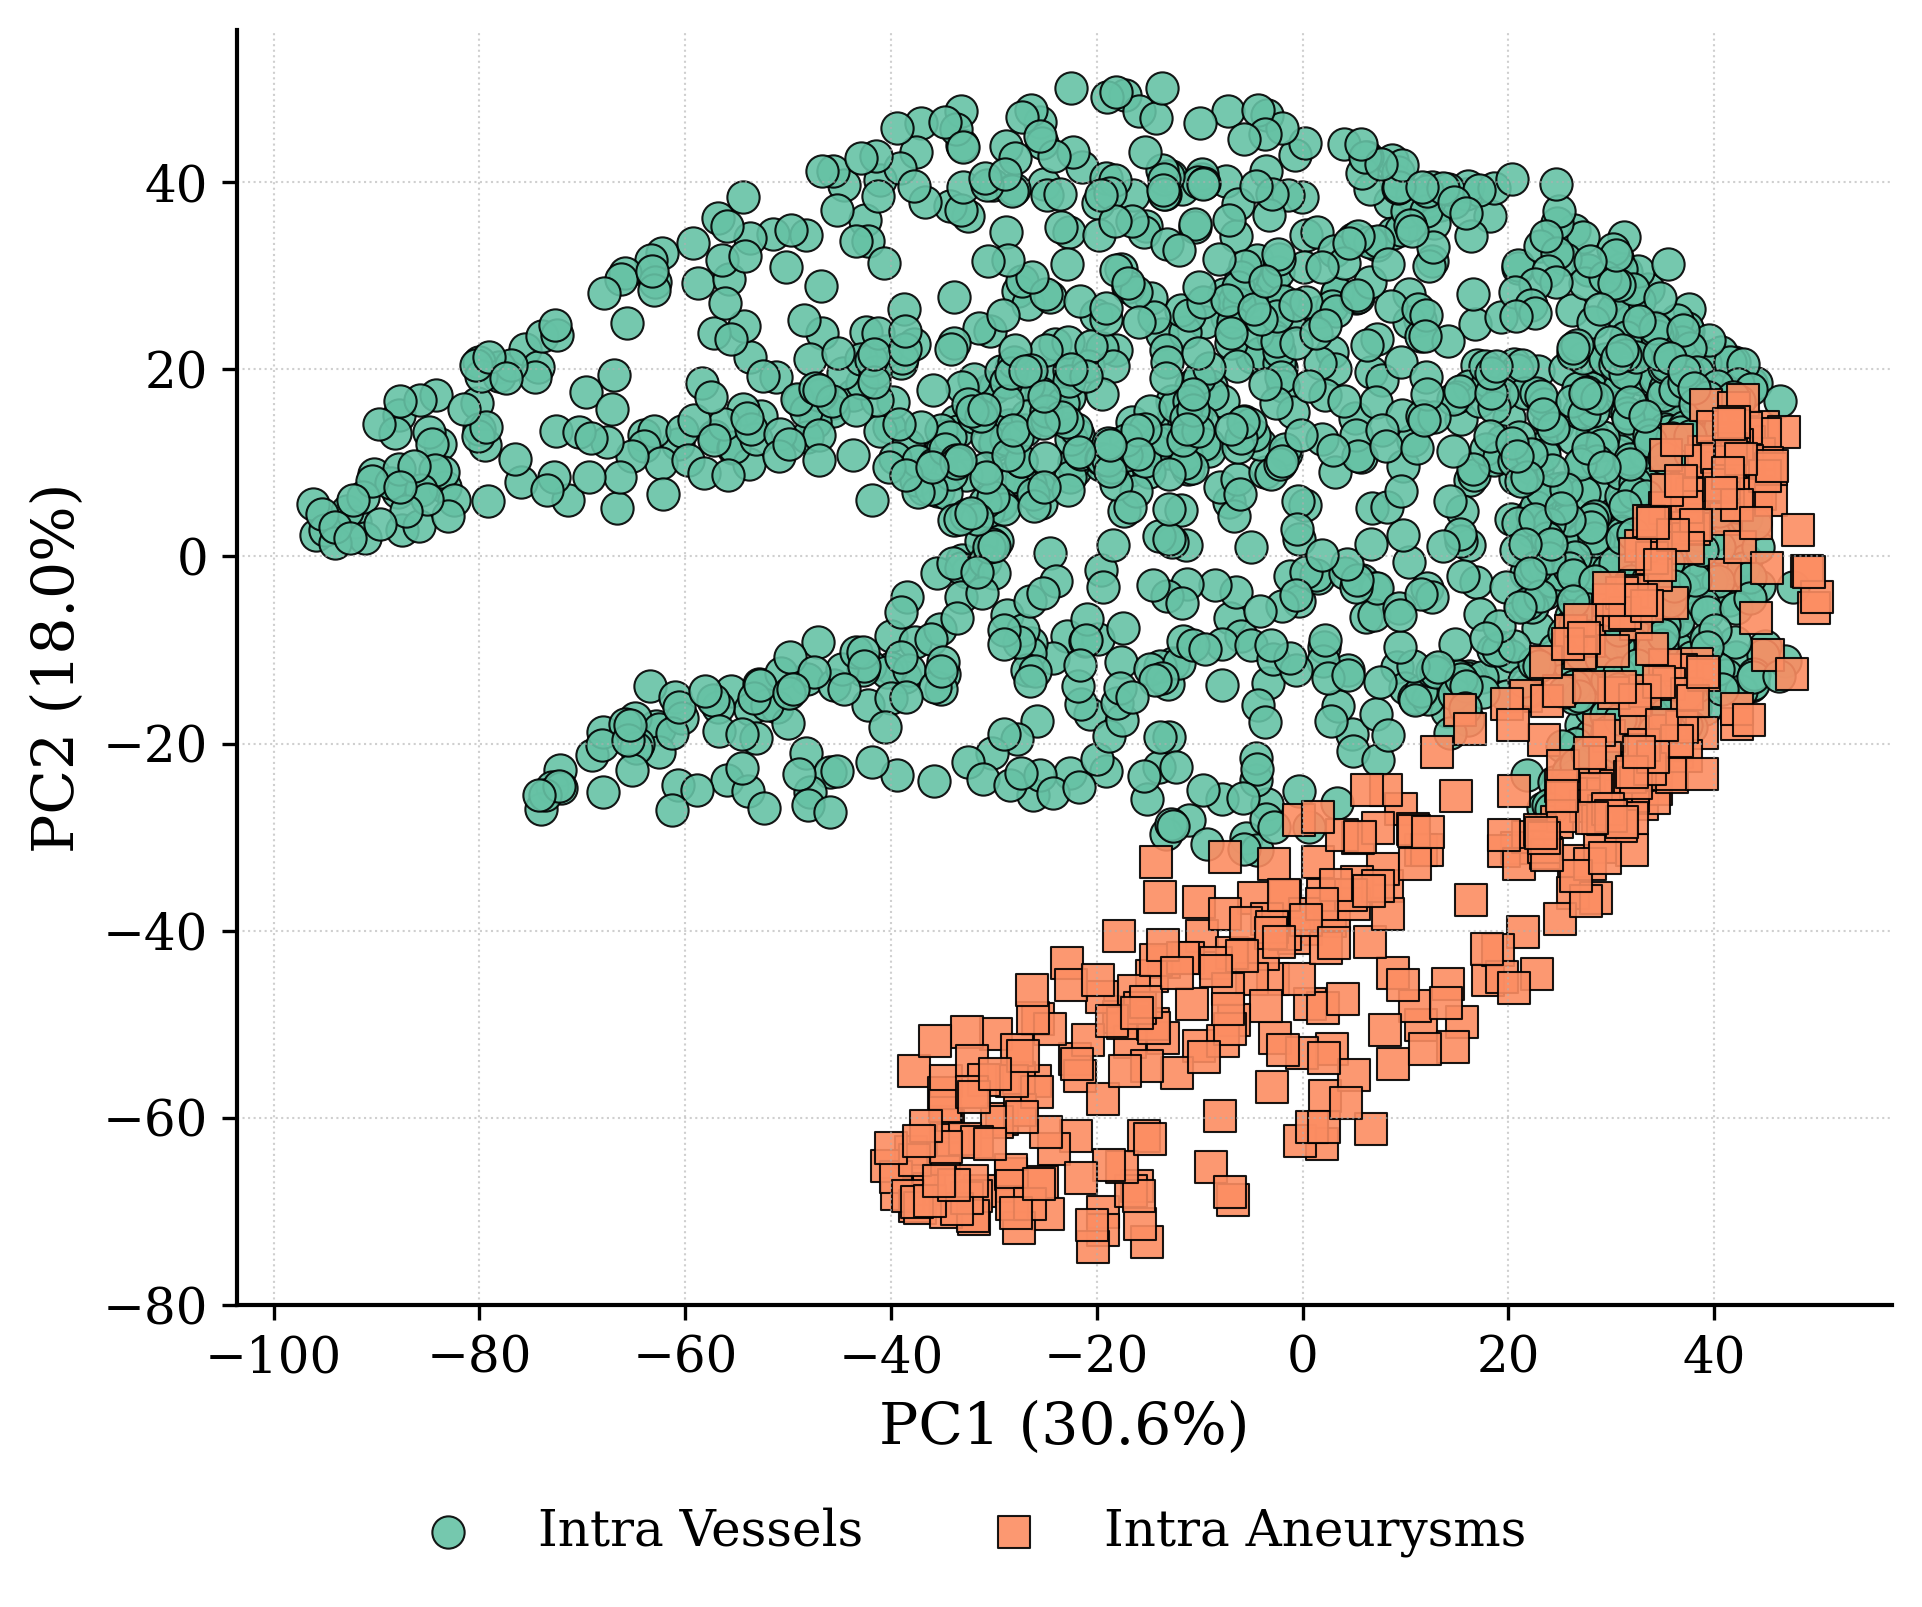
\includegraphics[width=0.34\textwidth]{pca_intra_features.png}
  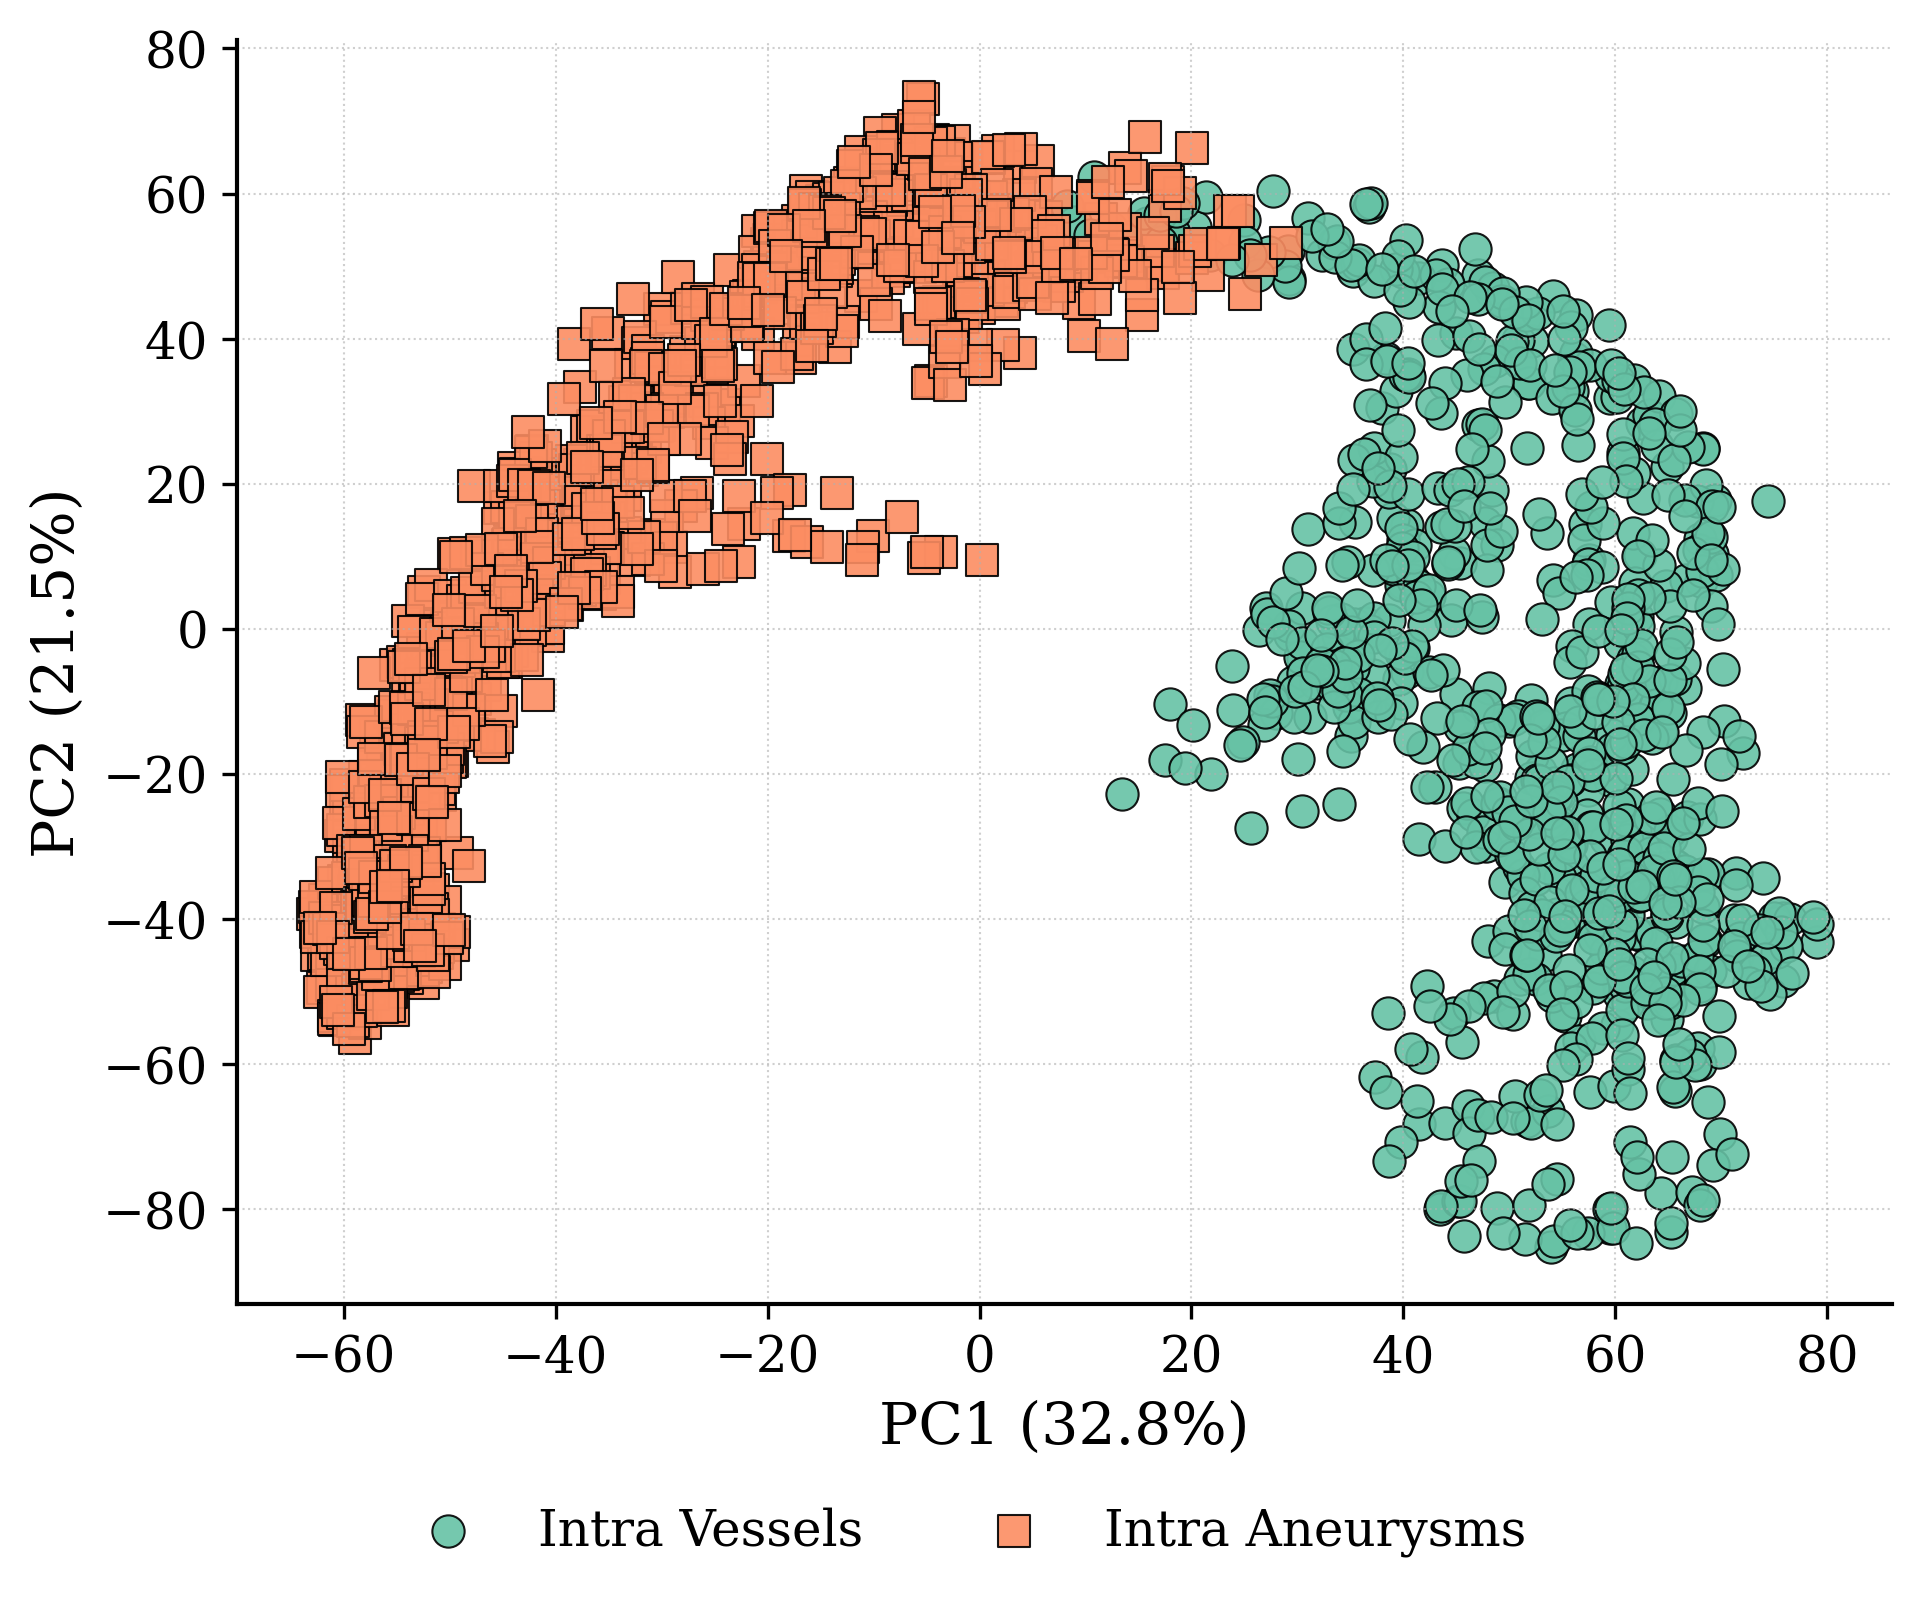
\includegraphics[width=0.34\textwidth]{pca_intra_features_2.png}
  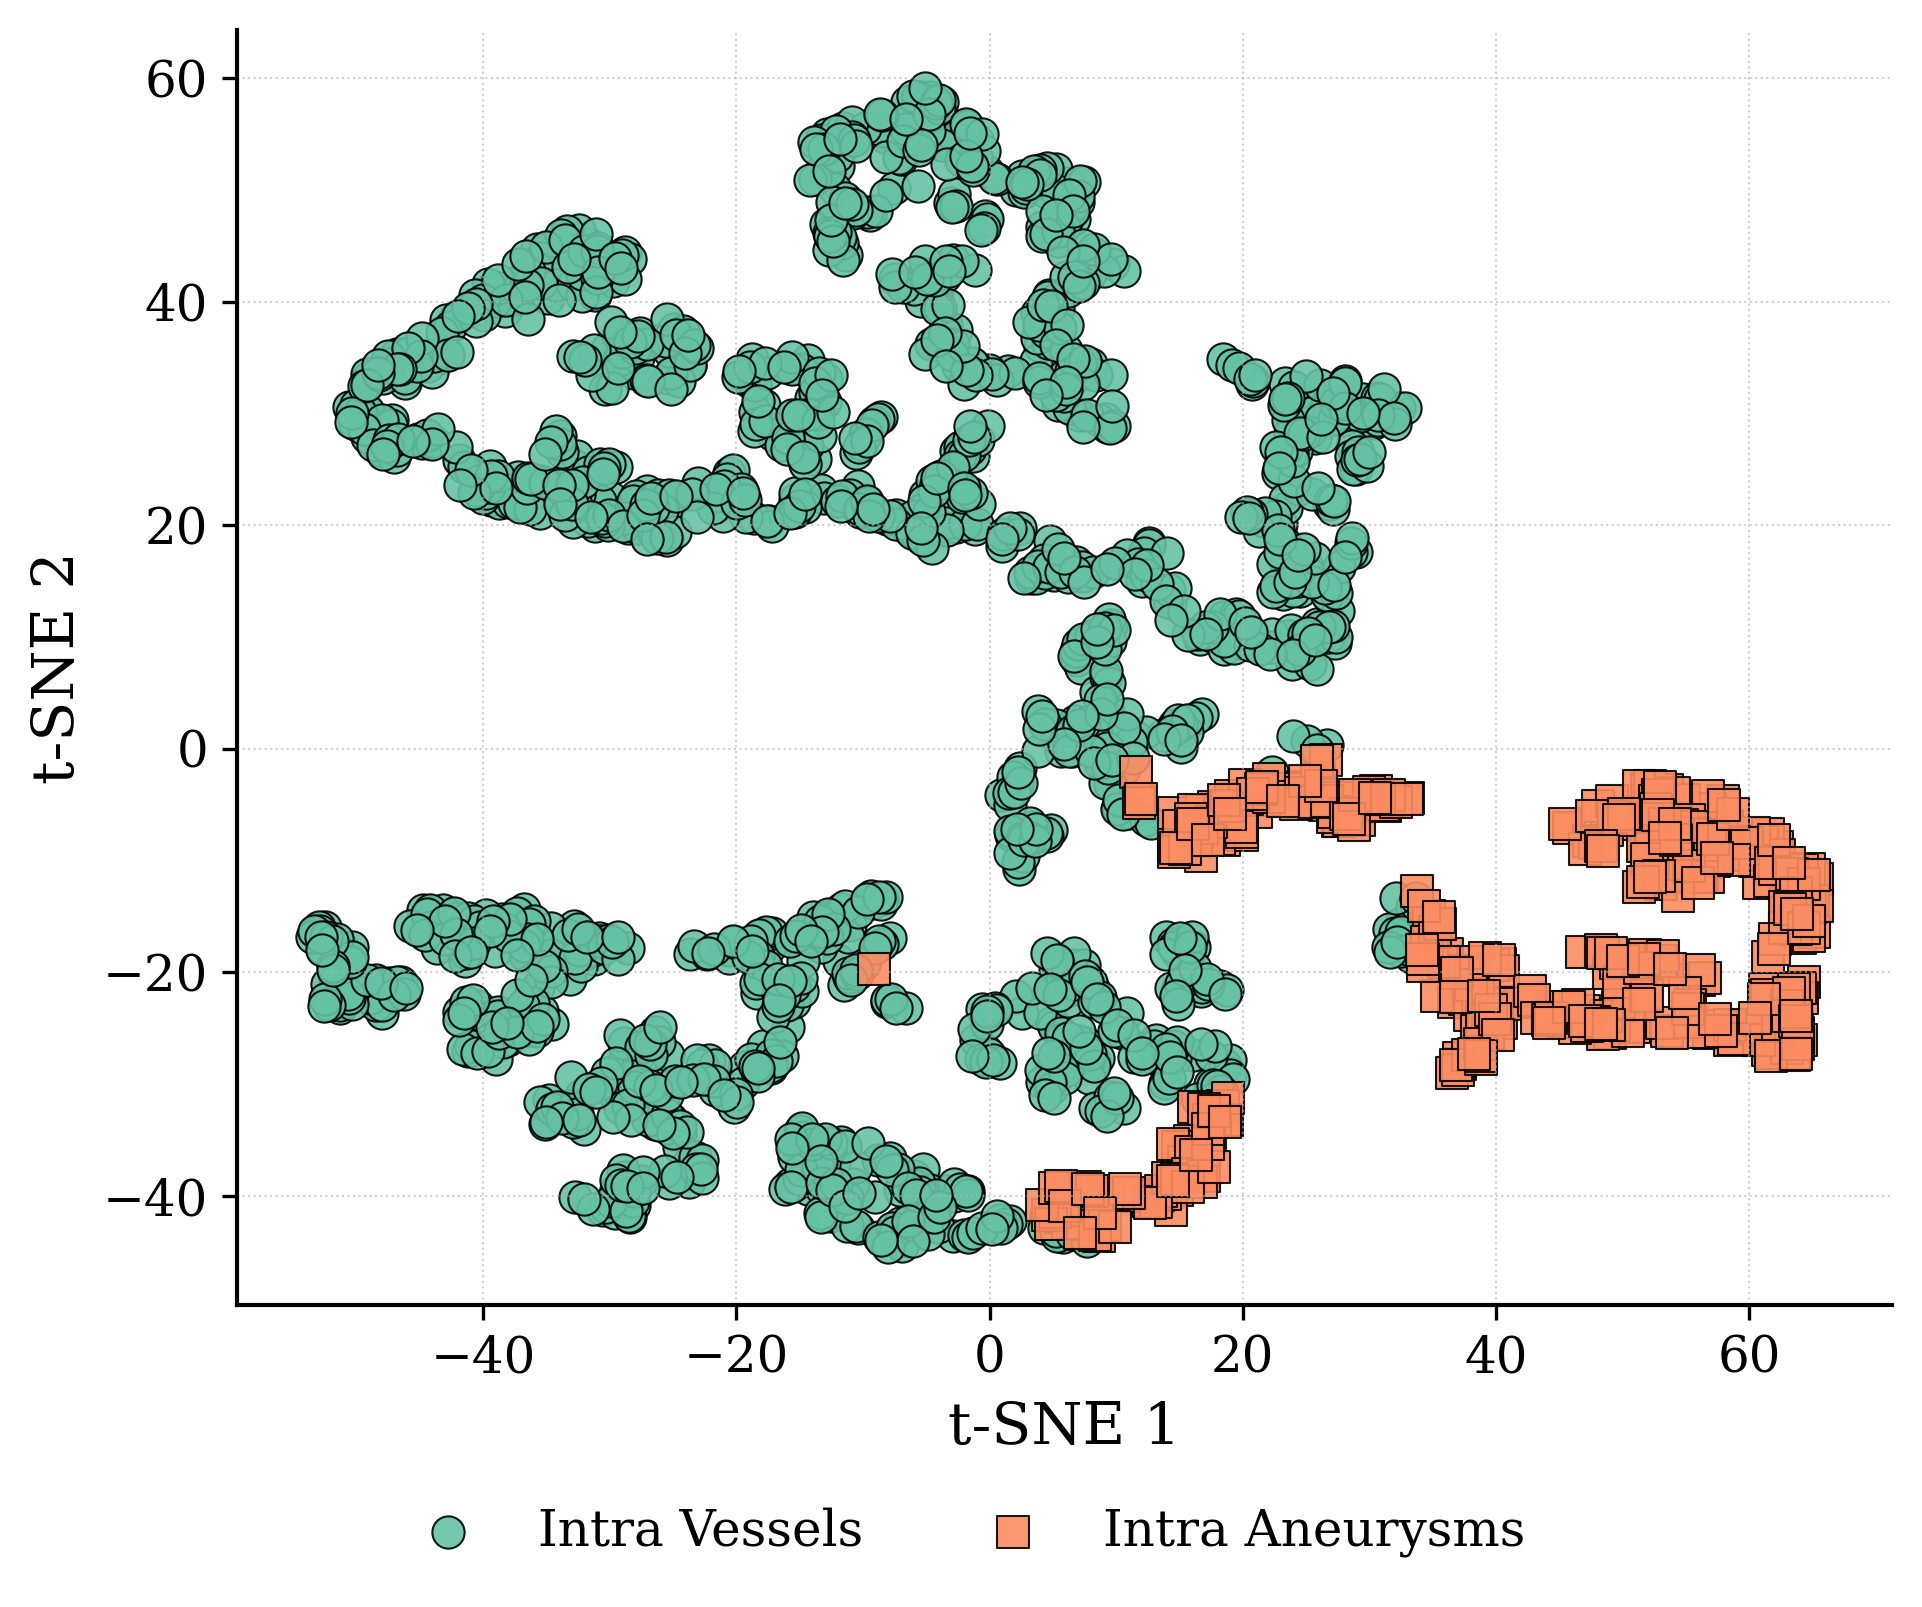
\includegraphics[width=0.34\textwidth]{t-sne_intra_features.png}
  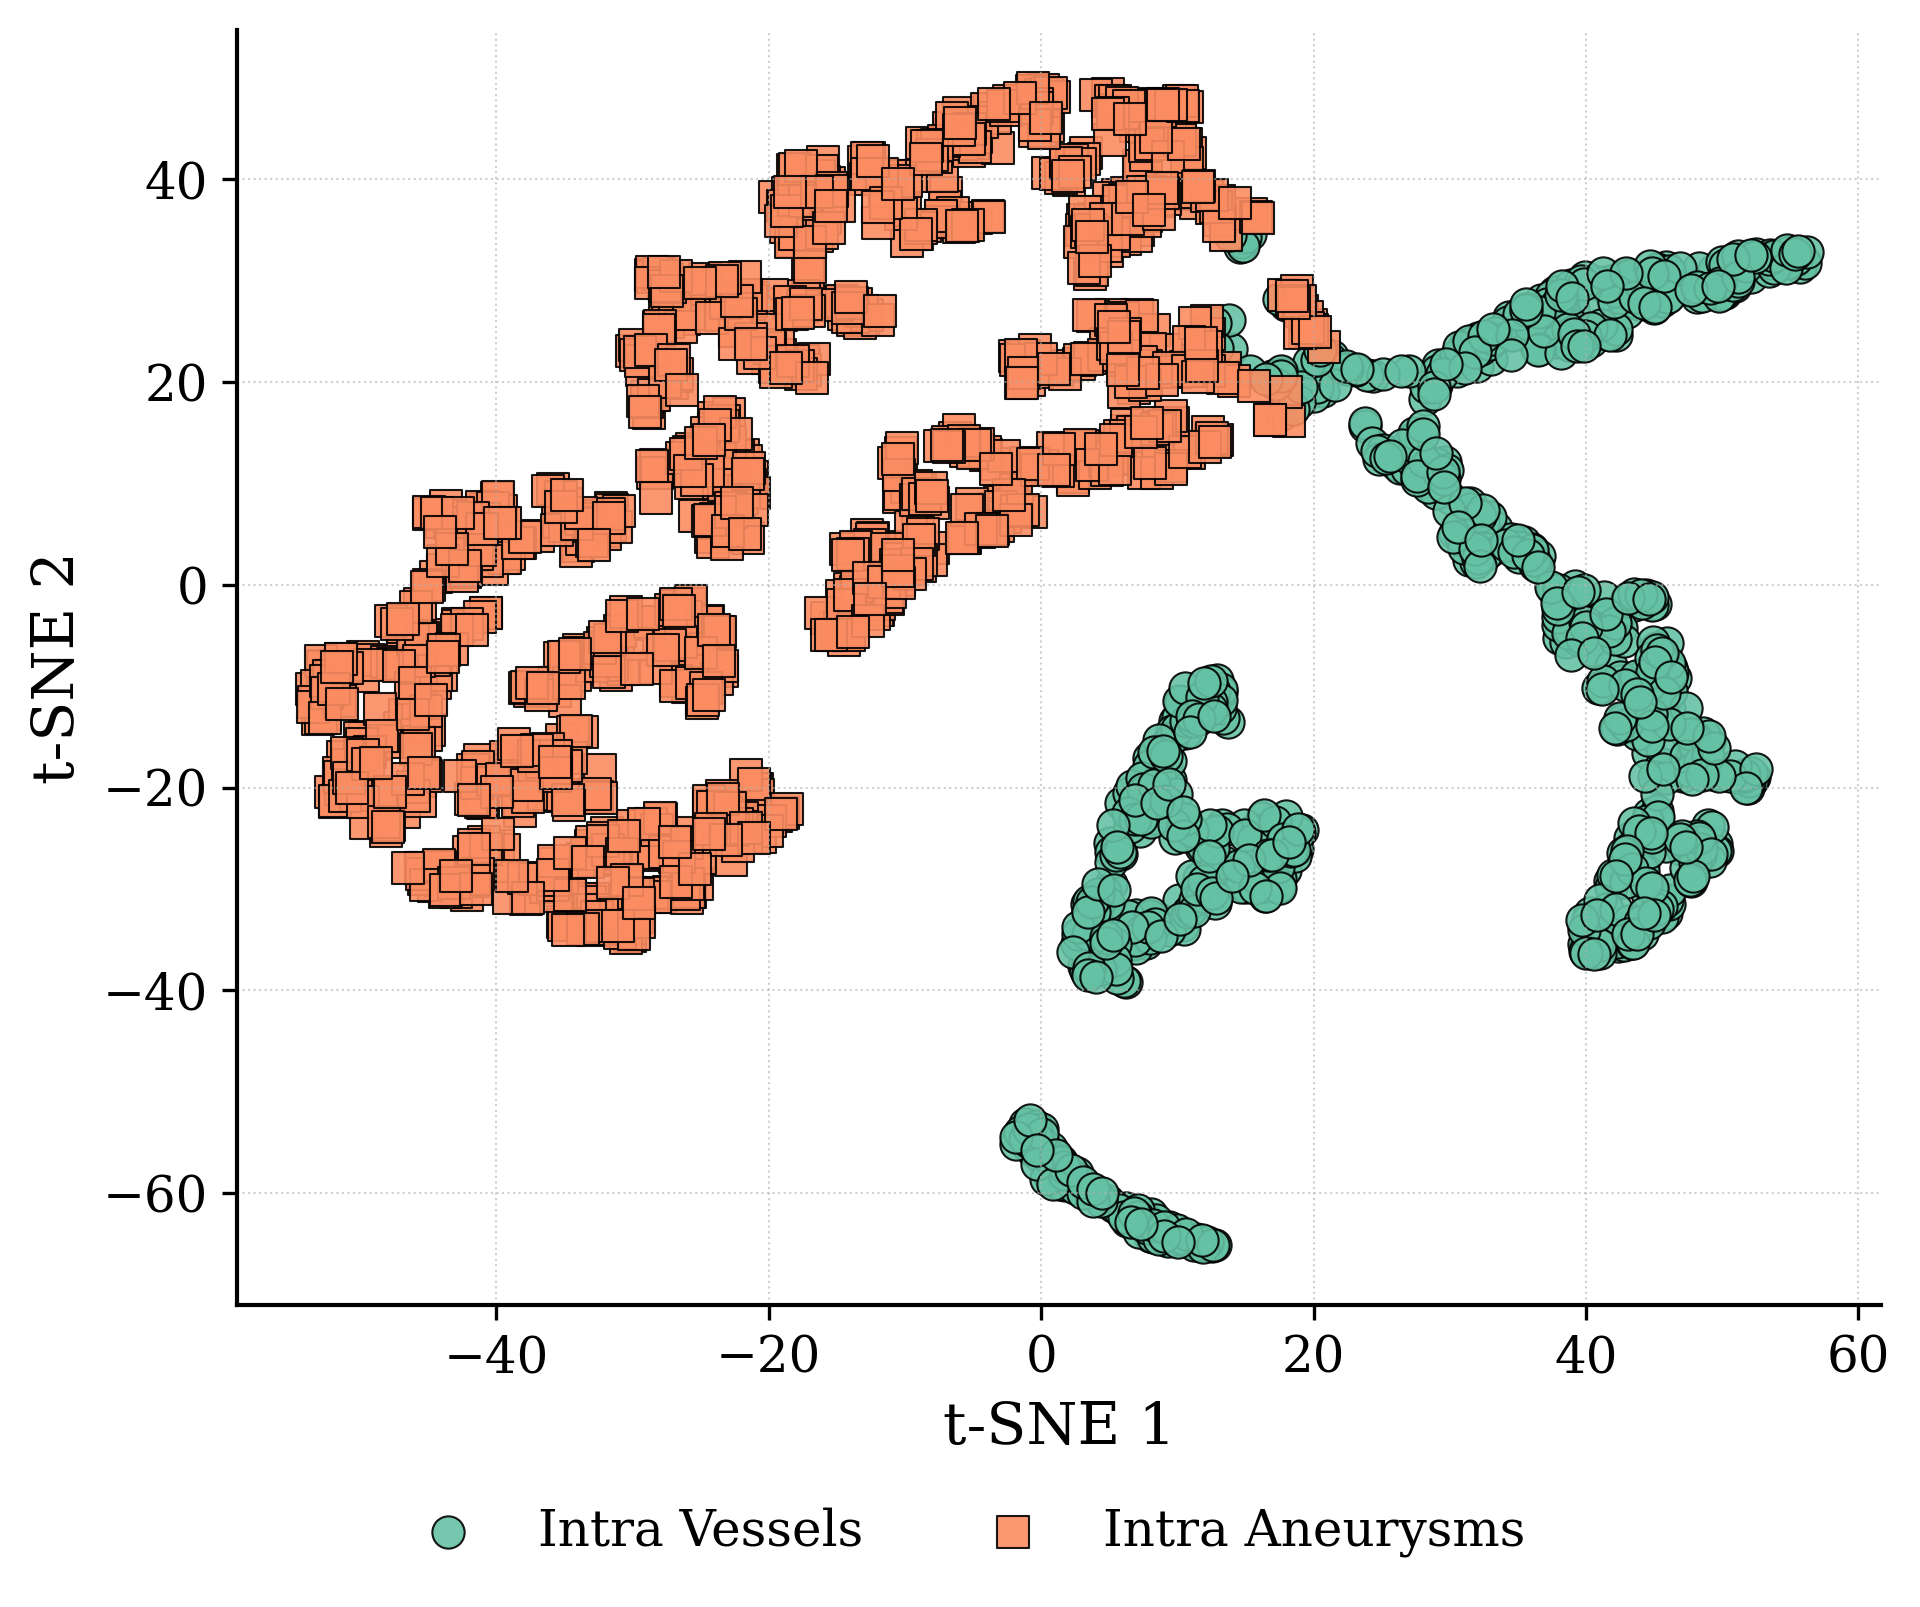
\includegraphics[width=0.34\textwidth]{t-sne_intra_features_2.png}
  \caption{t-SNE and PCA on all points of two different aneurysms from the Intra 3D segmentation dataset. The first two figures show the PCA components, while the last two figures show the t-SNE components.}
  \label{fig:seg_all}
\end{figure}

\begin{figure}[h!]
  \centering
  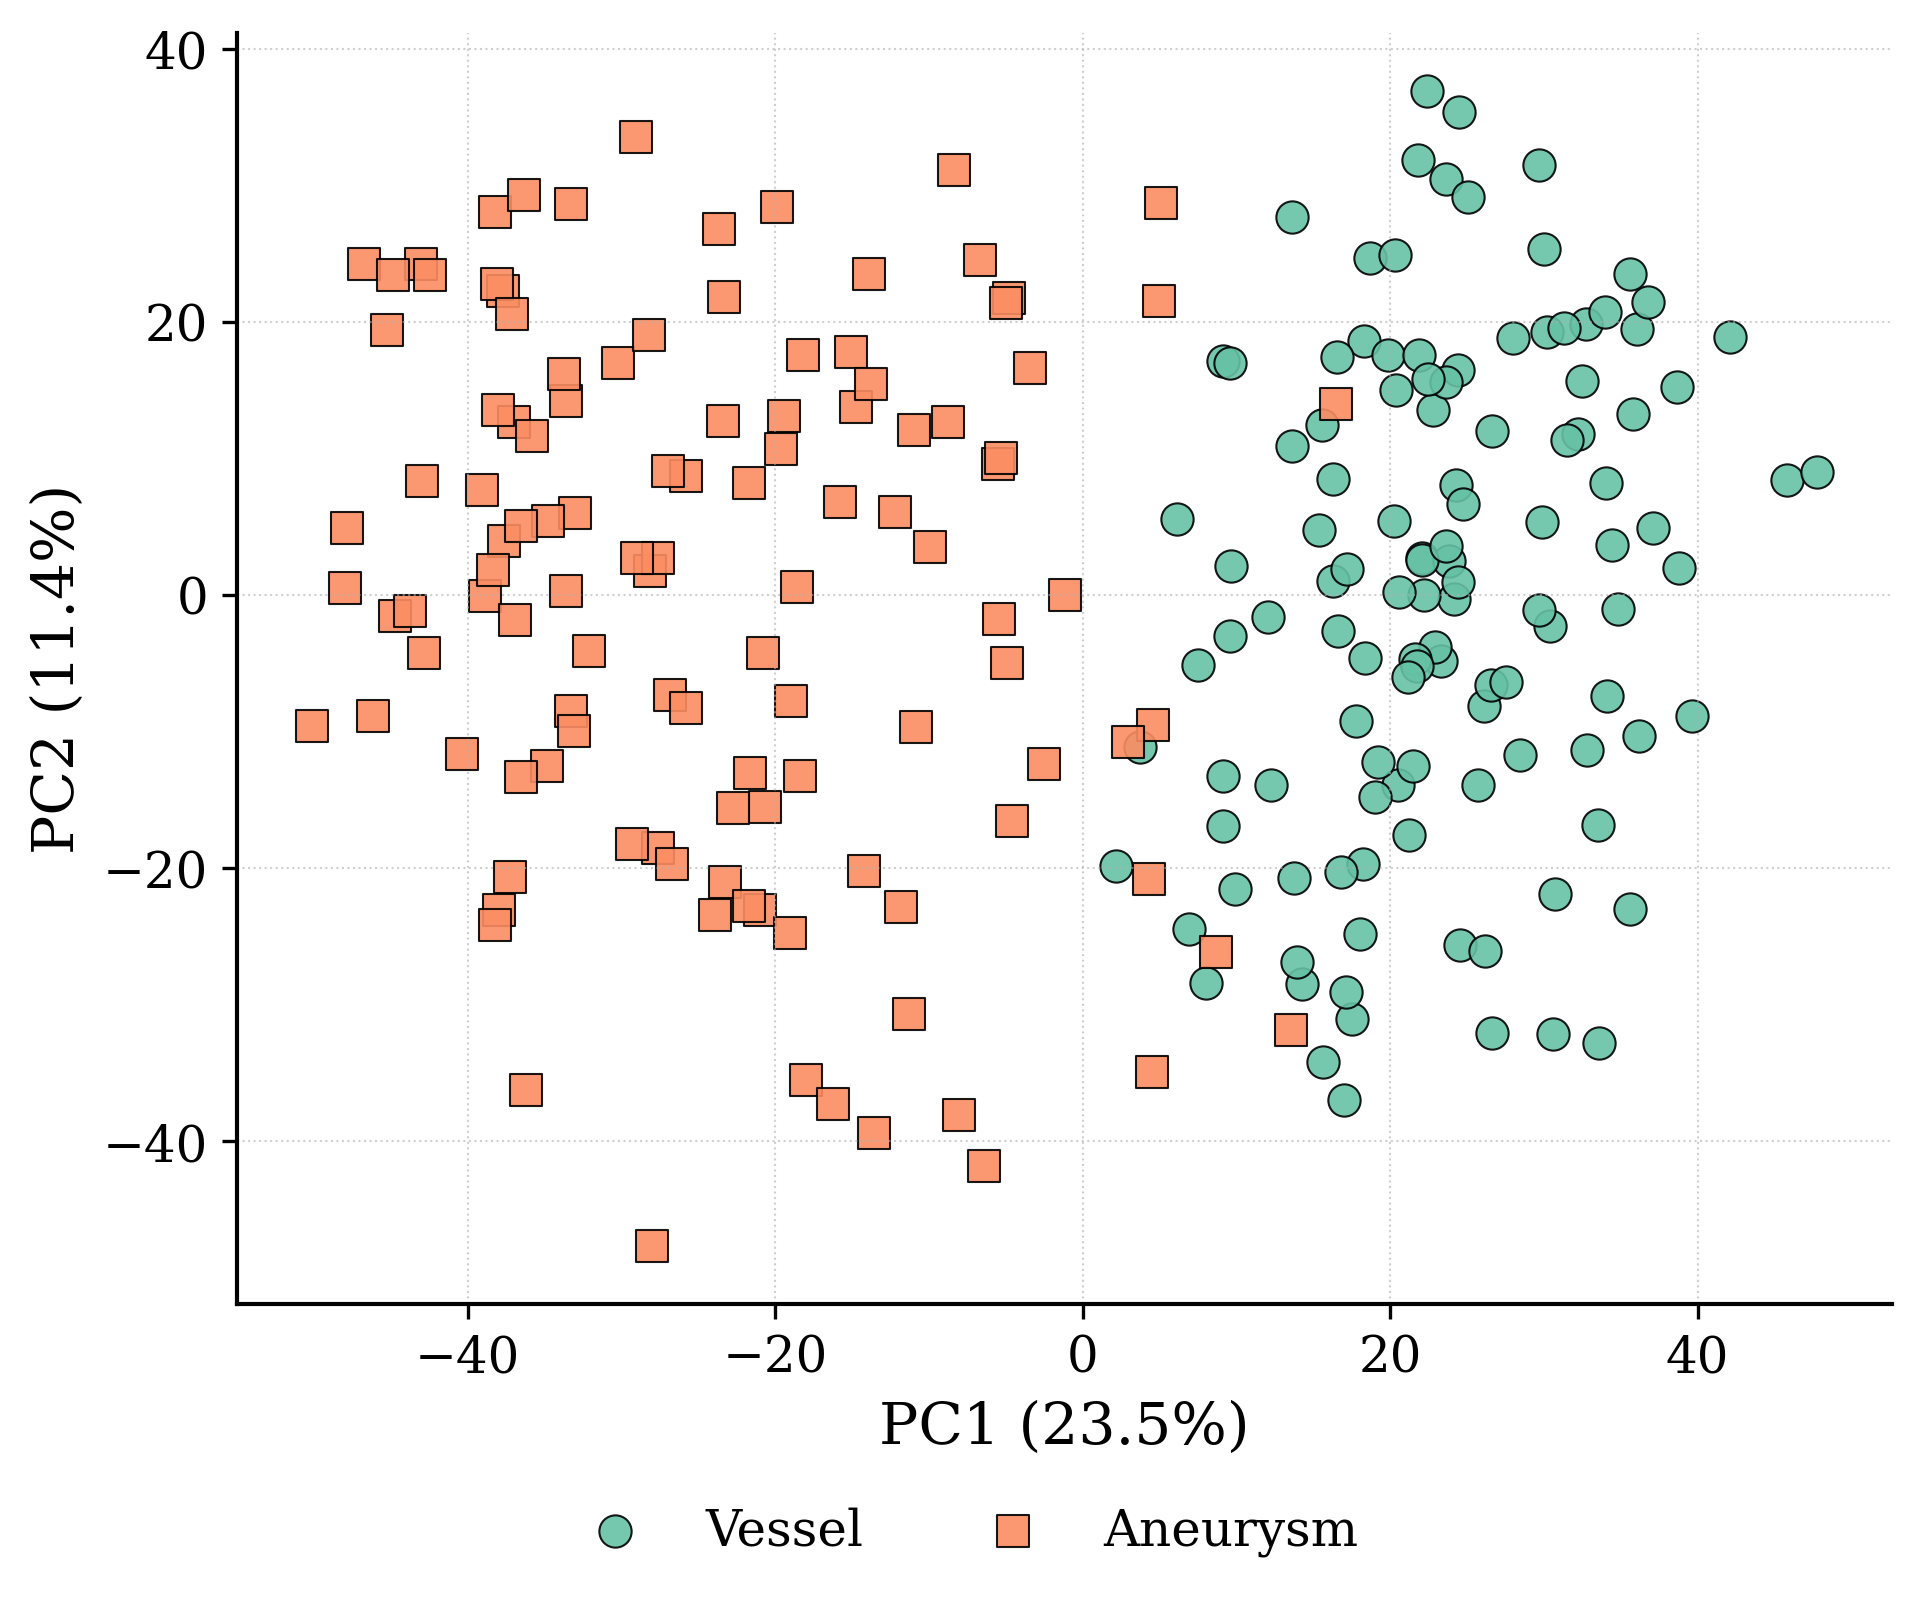
\includegraphics[width=0.34\textwidth]{pca_global_mean.png}
  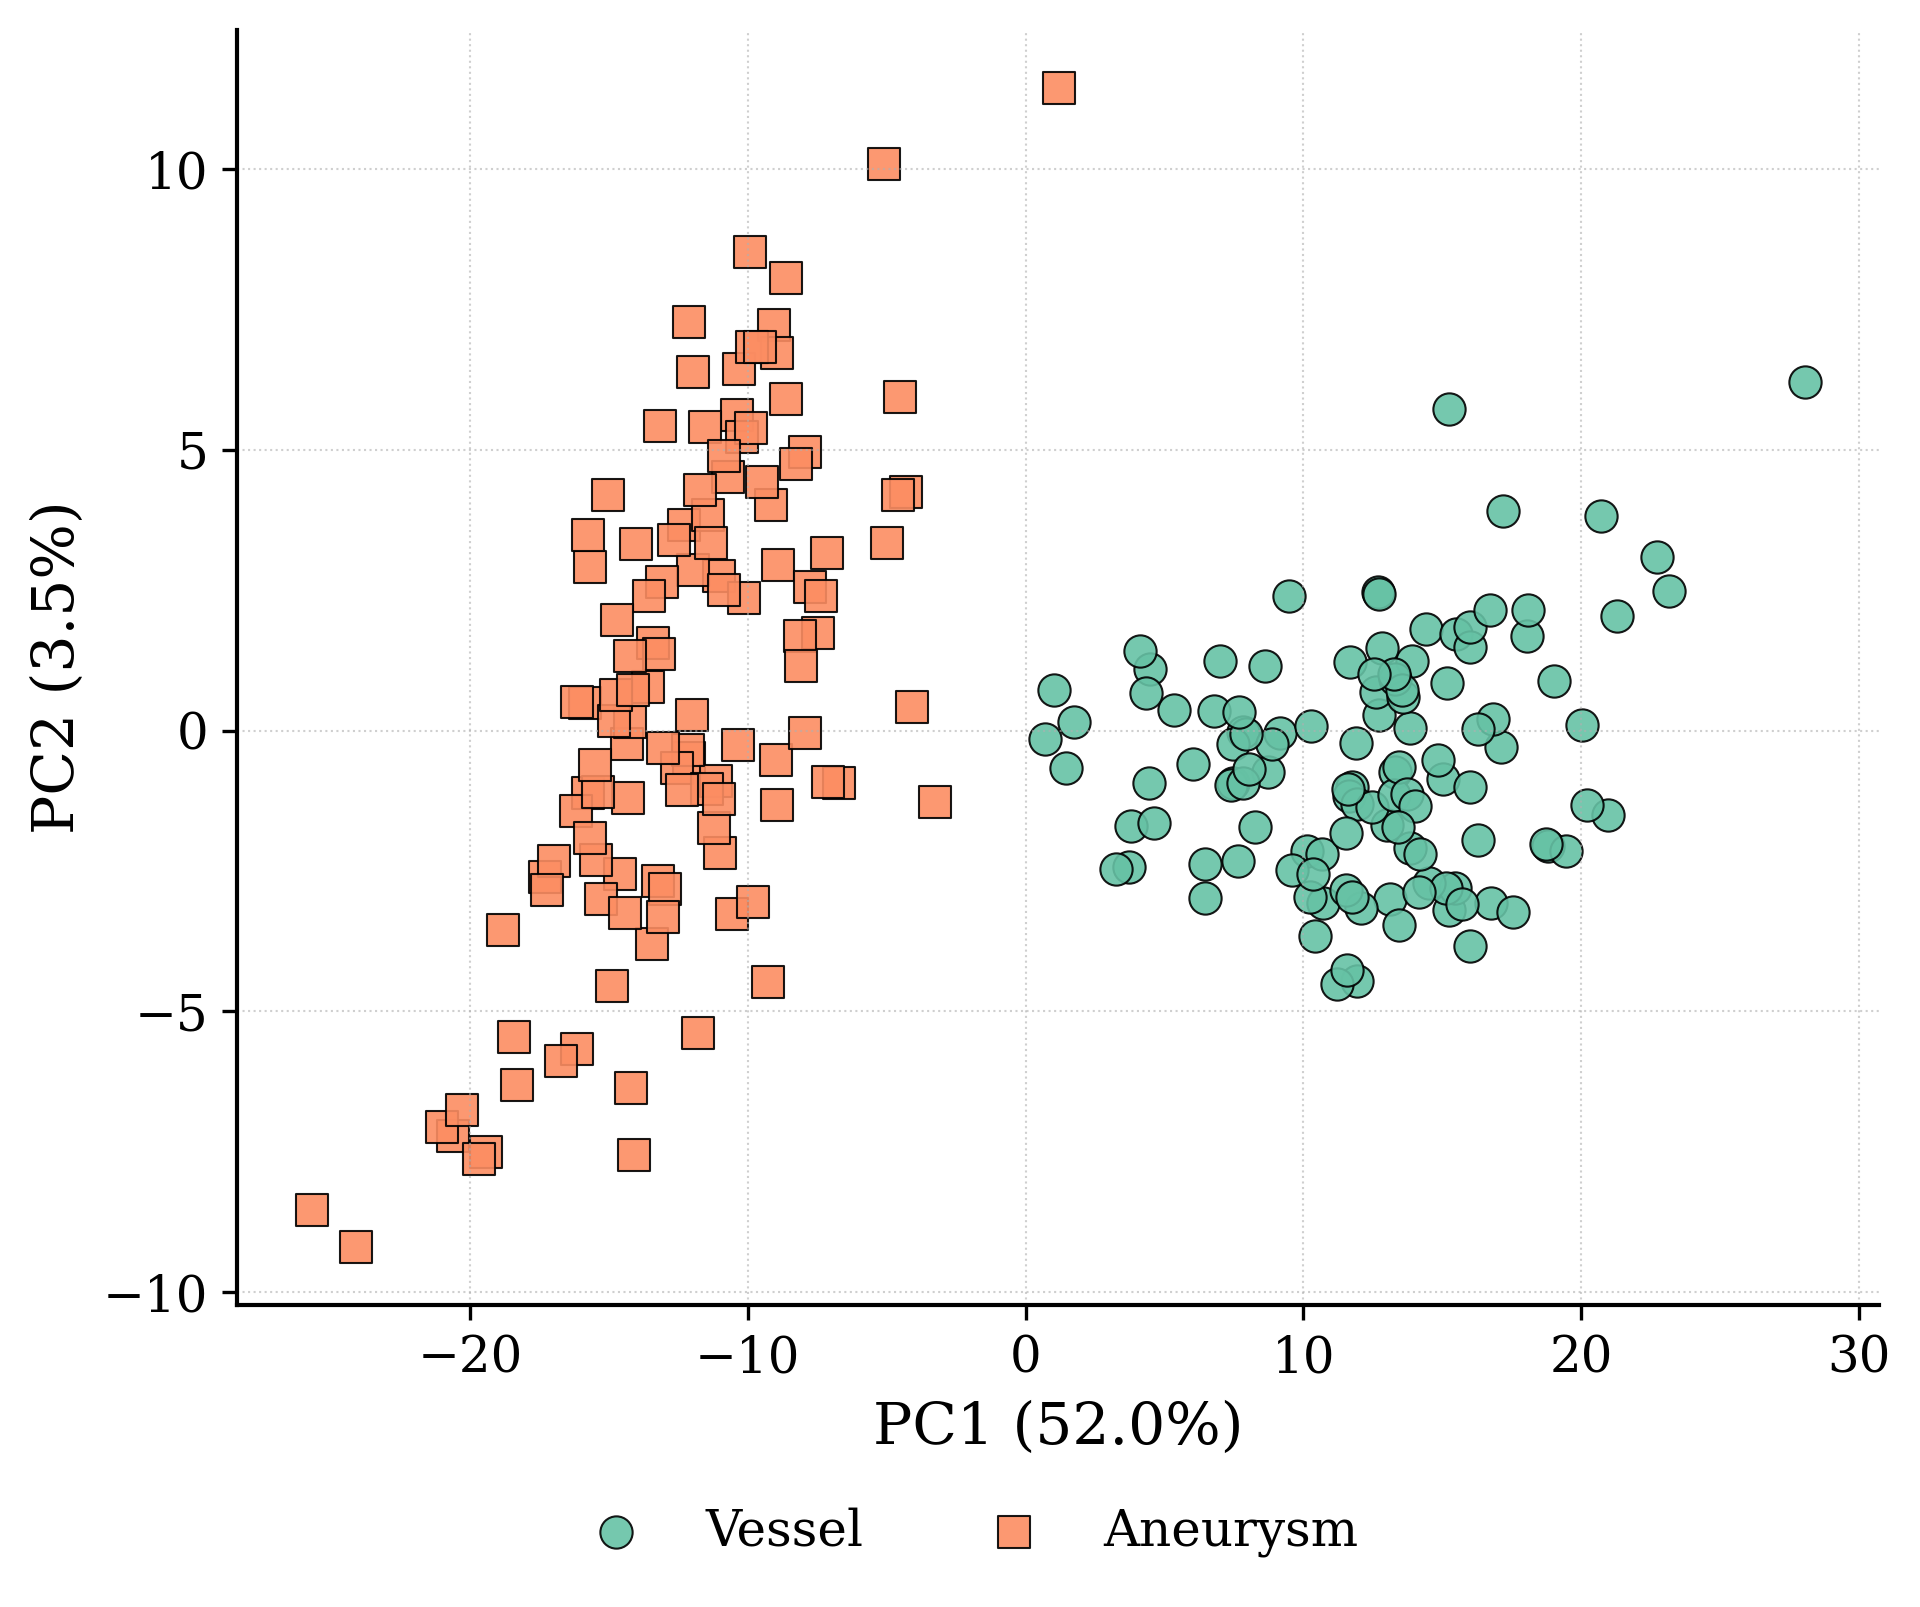
\includegraphics[width=0.34\textwidth]{pca_global_std.png}
  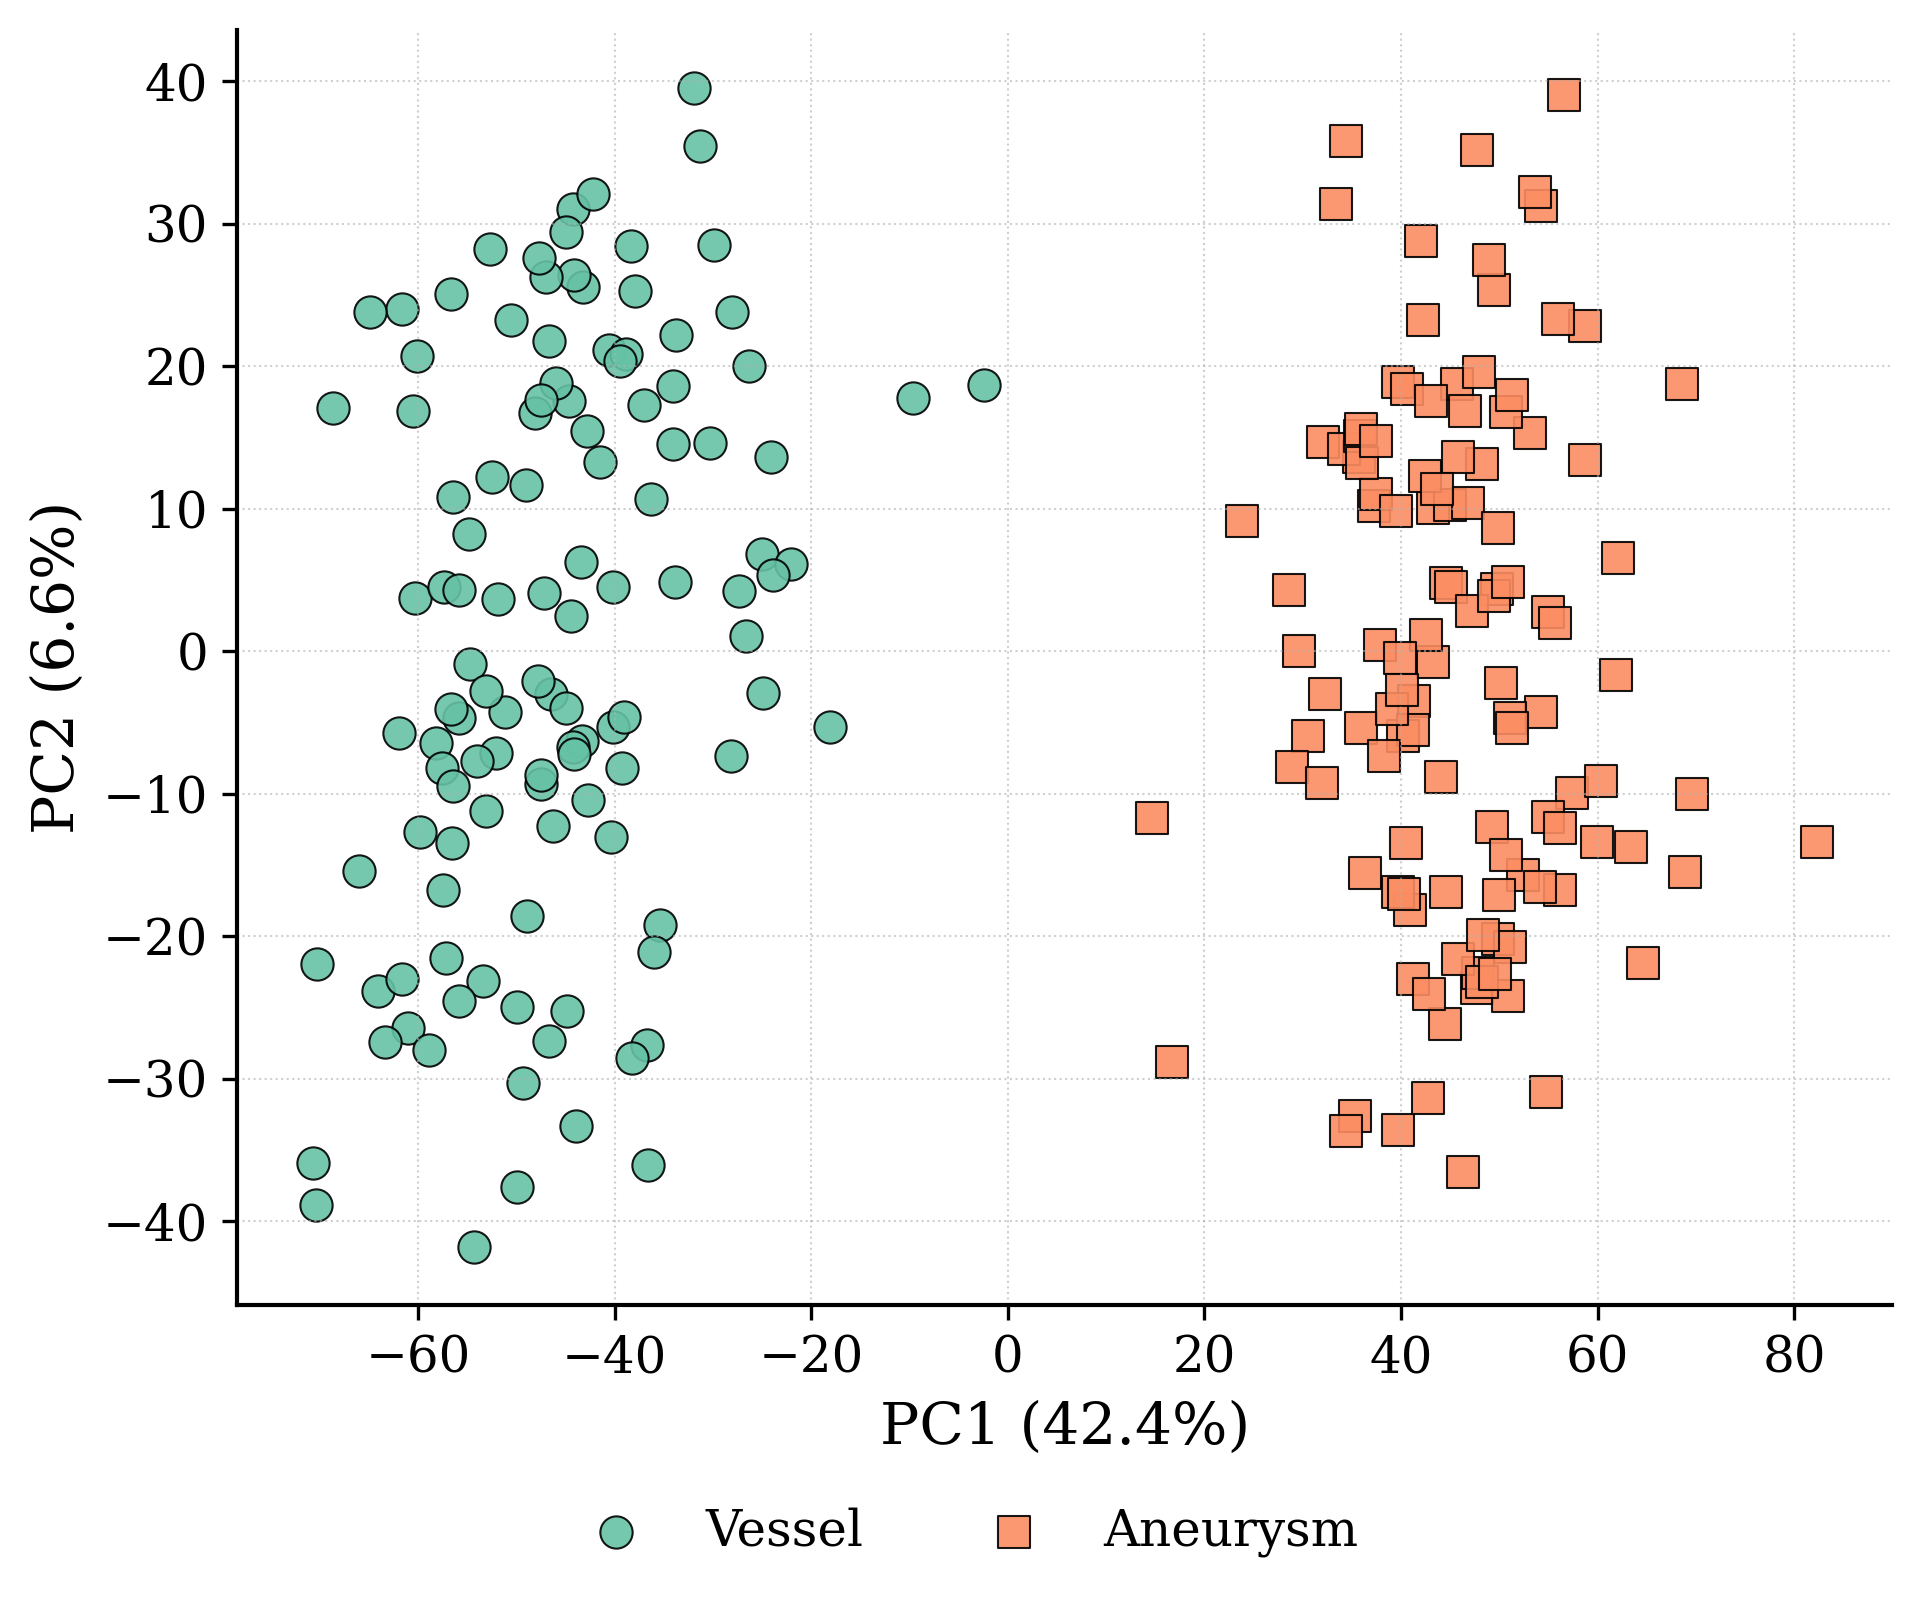
\includegraphics[width=0.34\textwidth]{pca_global_min.png}
  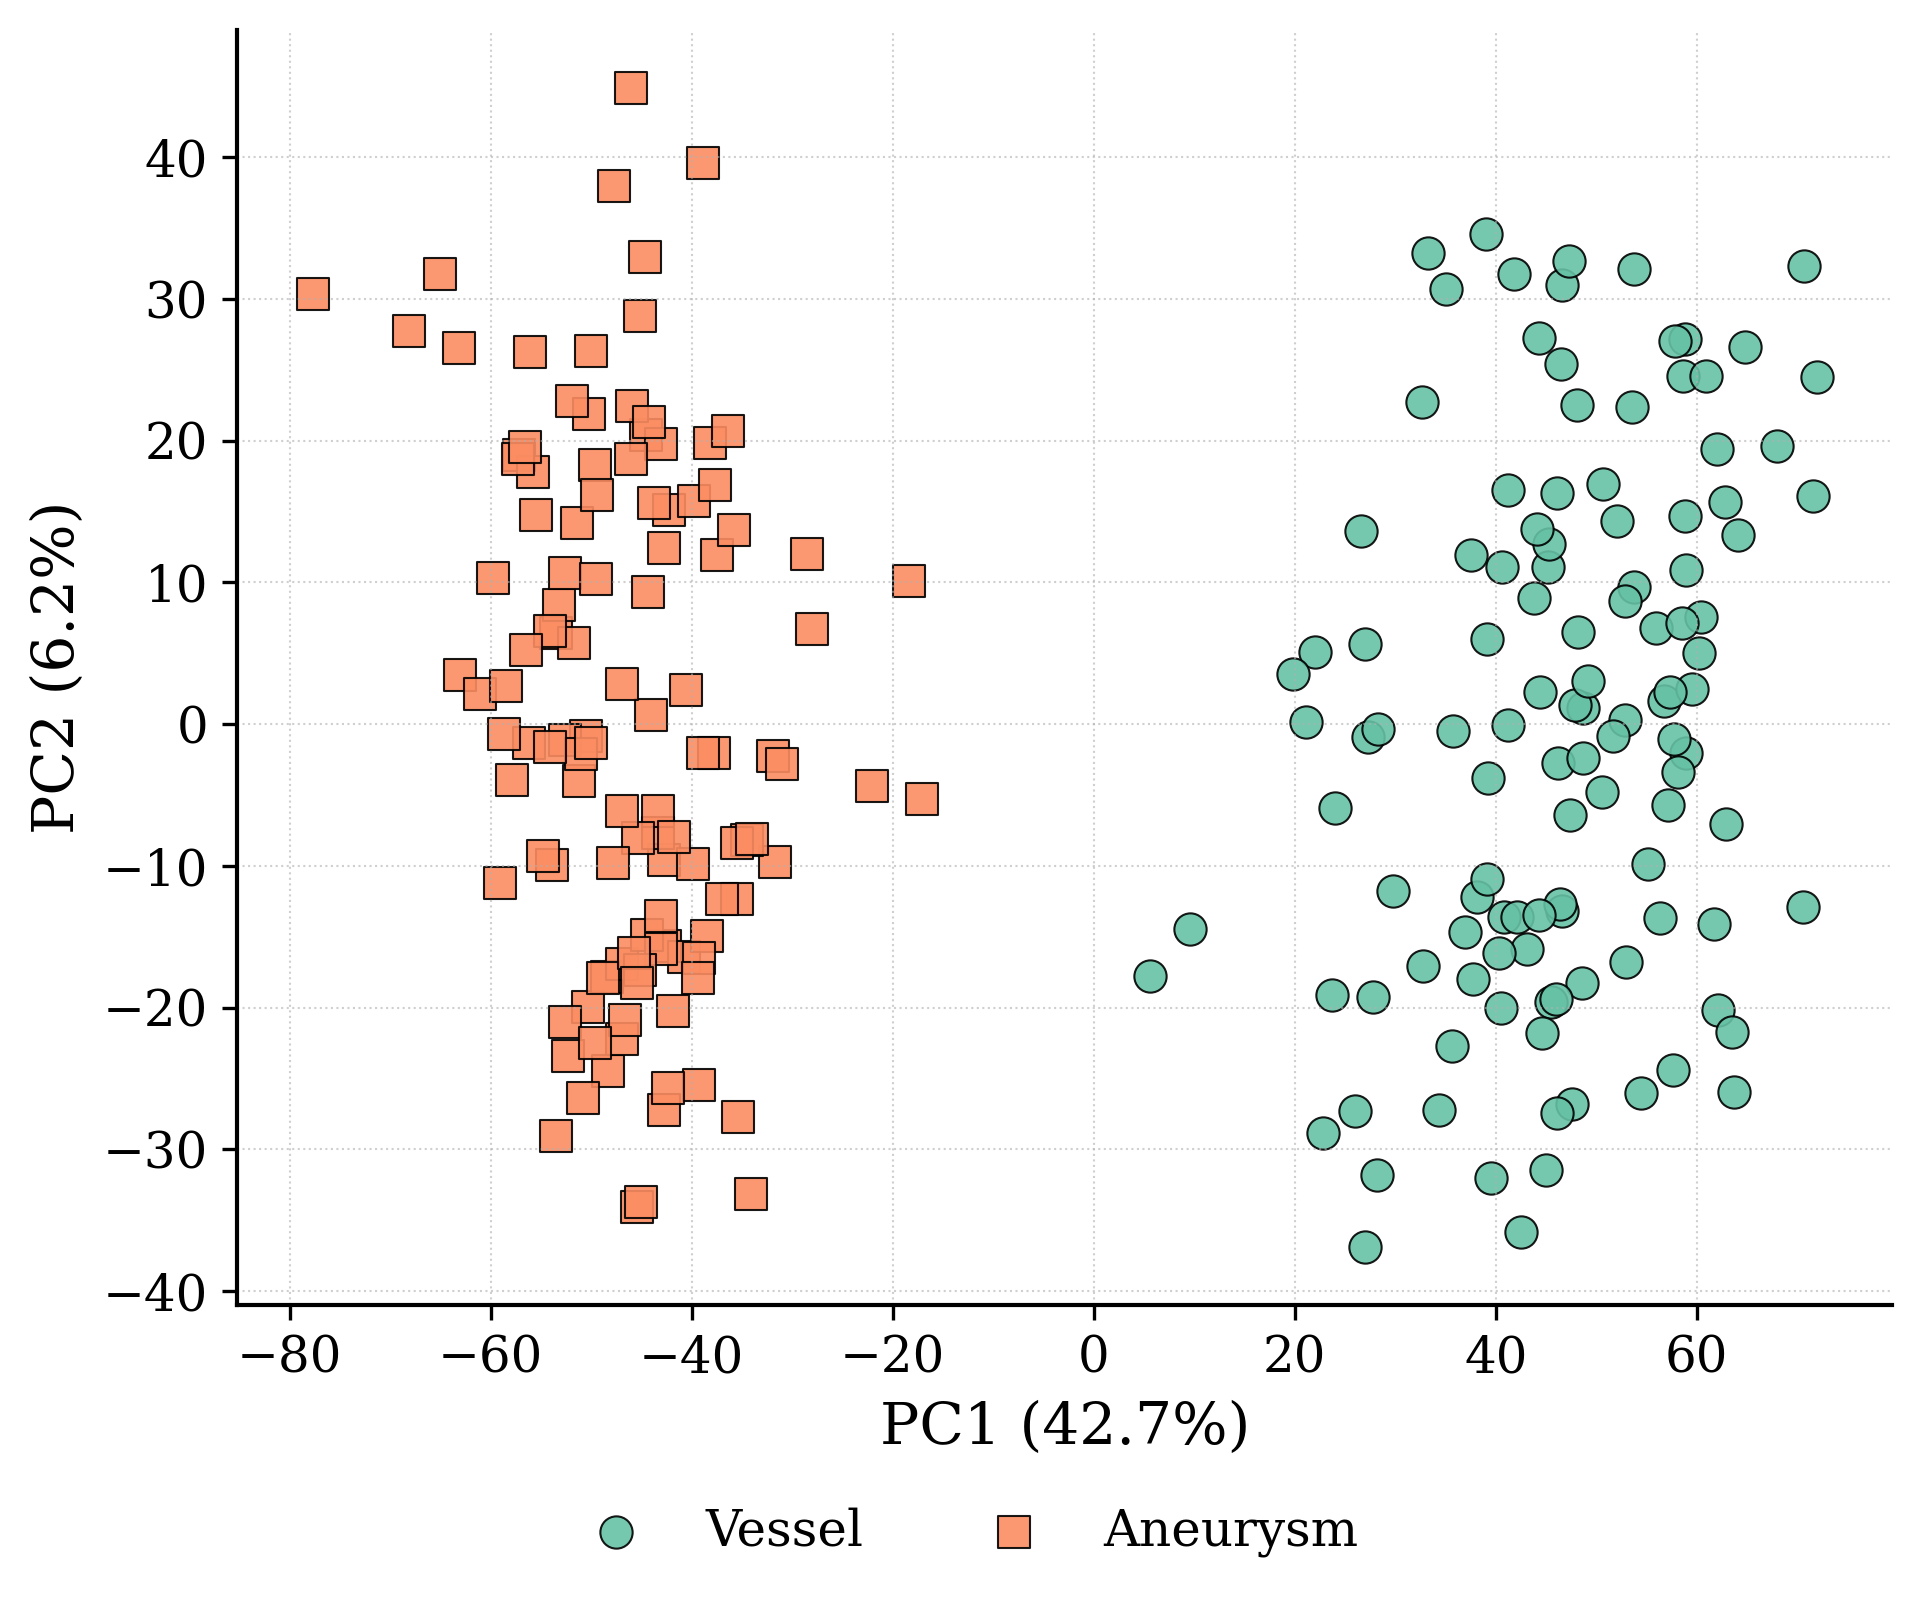
\includegraphics[width=0.34\textwidth]{pca_global_max.png}
  \caption{Results of PCA on annotated aneurysms over the Intra3D segmentation dataset. Figures show the mean, standard deviation, minimum, and maximum of the PCA components of the aneurysm and the vessel parts.}
  \label{fig:aneu_seg_supplementary}
\end{figure}

\begin{figure}[h!]
  \centering
  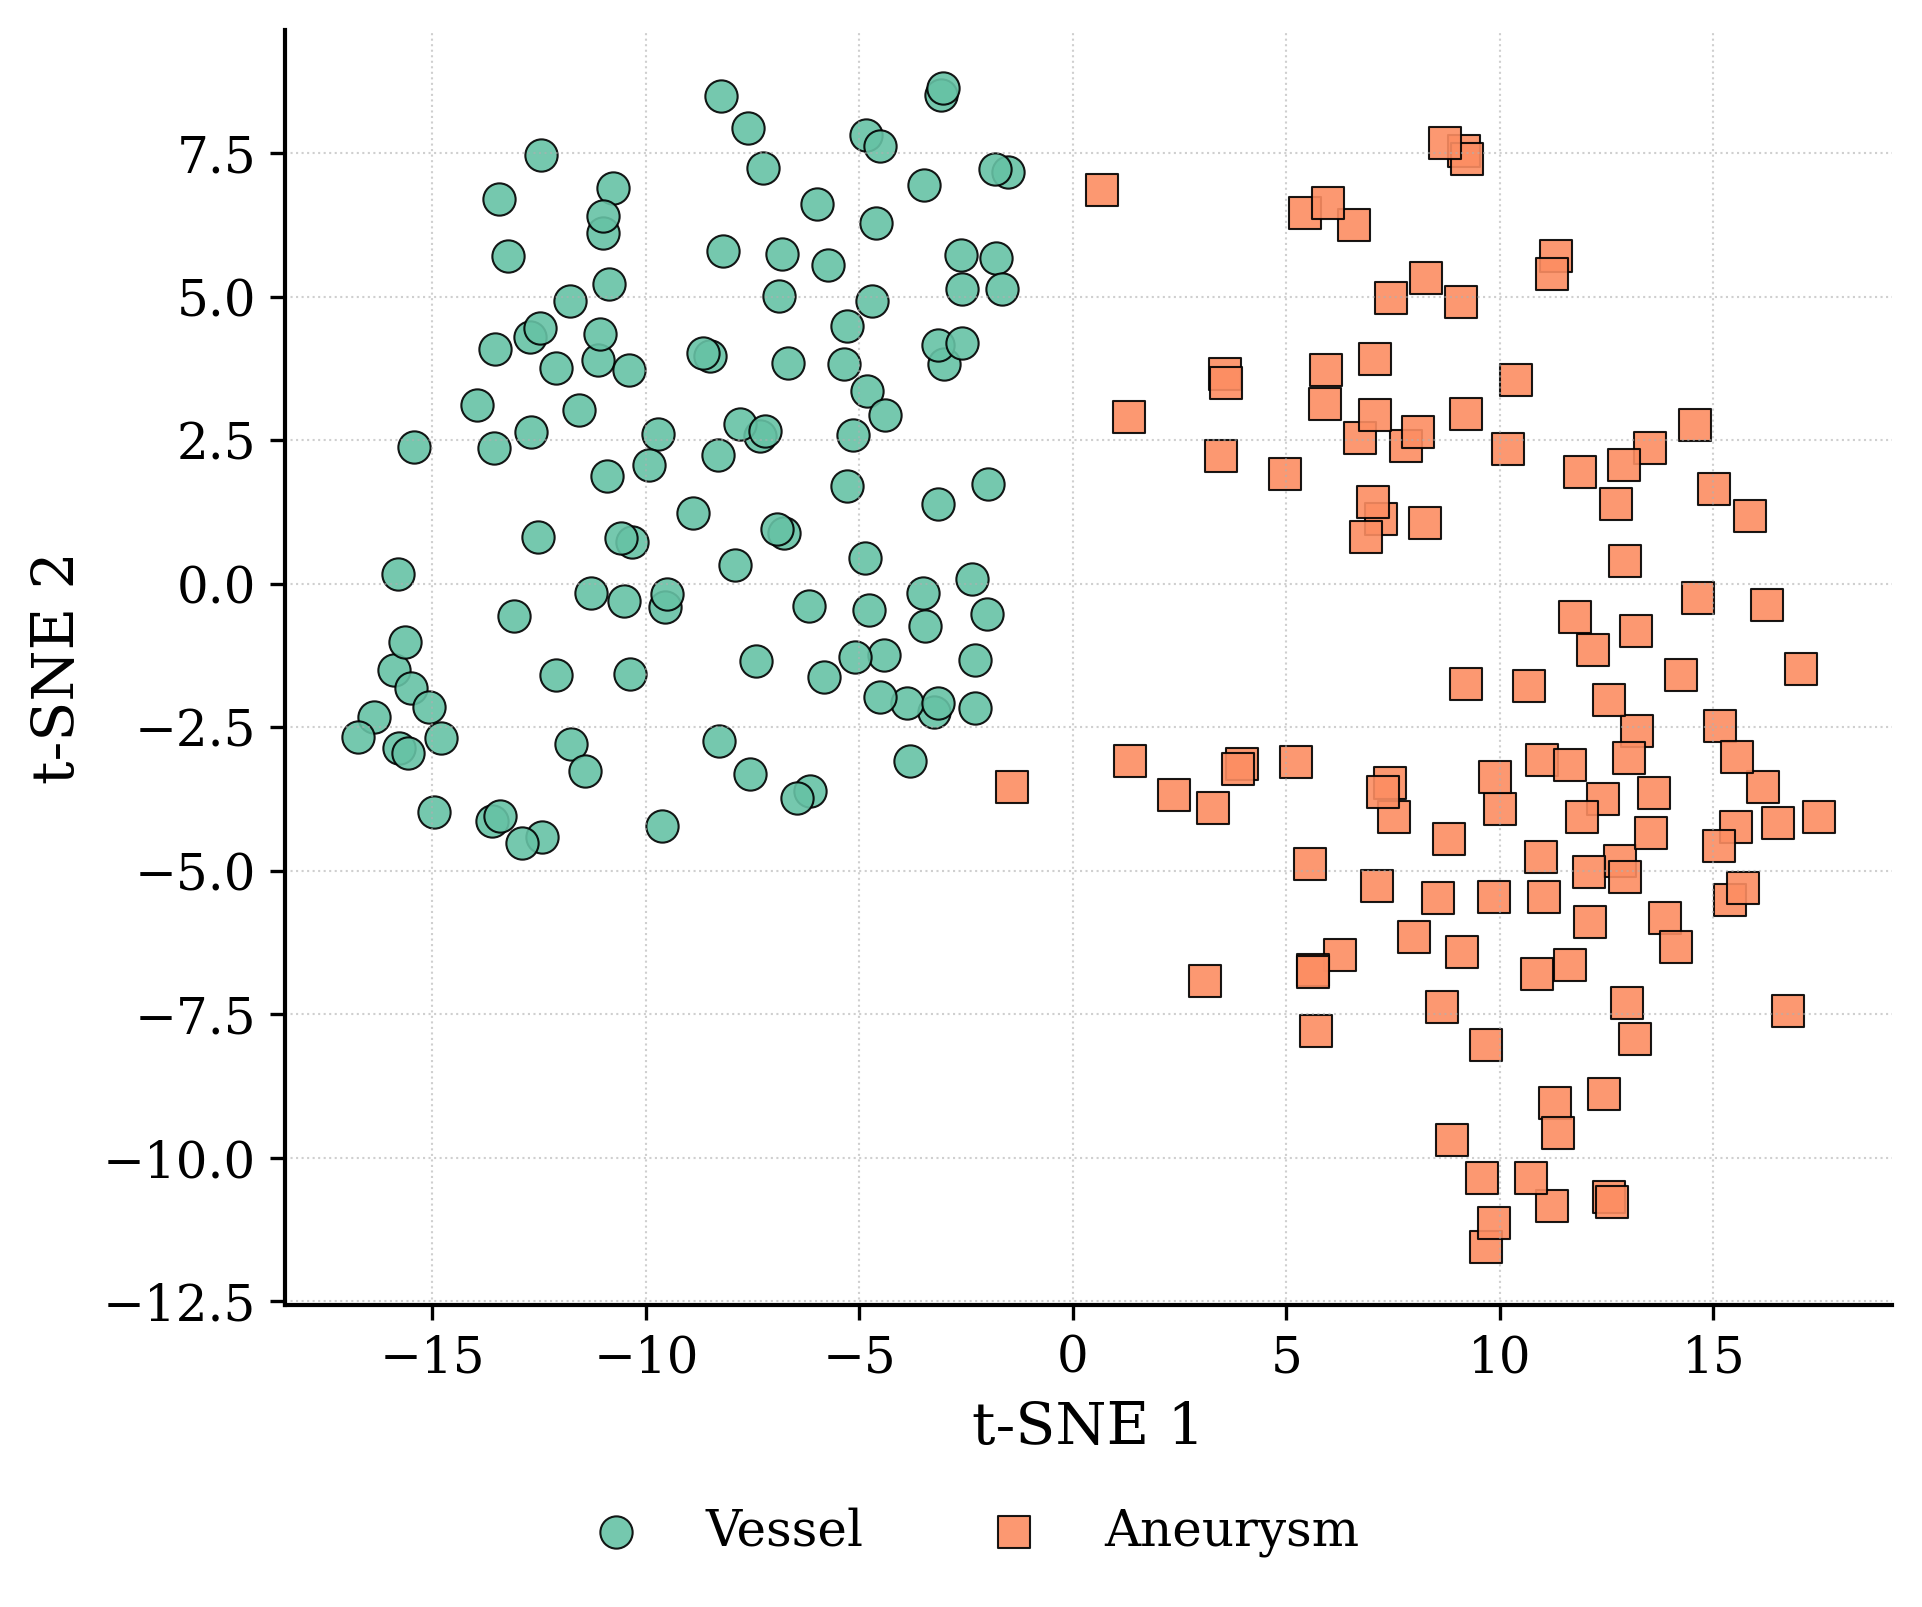
\includegraphics[width=0.34\textwidth]{t-sne_global_mean.png}
  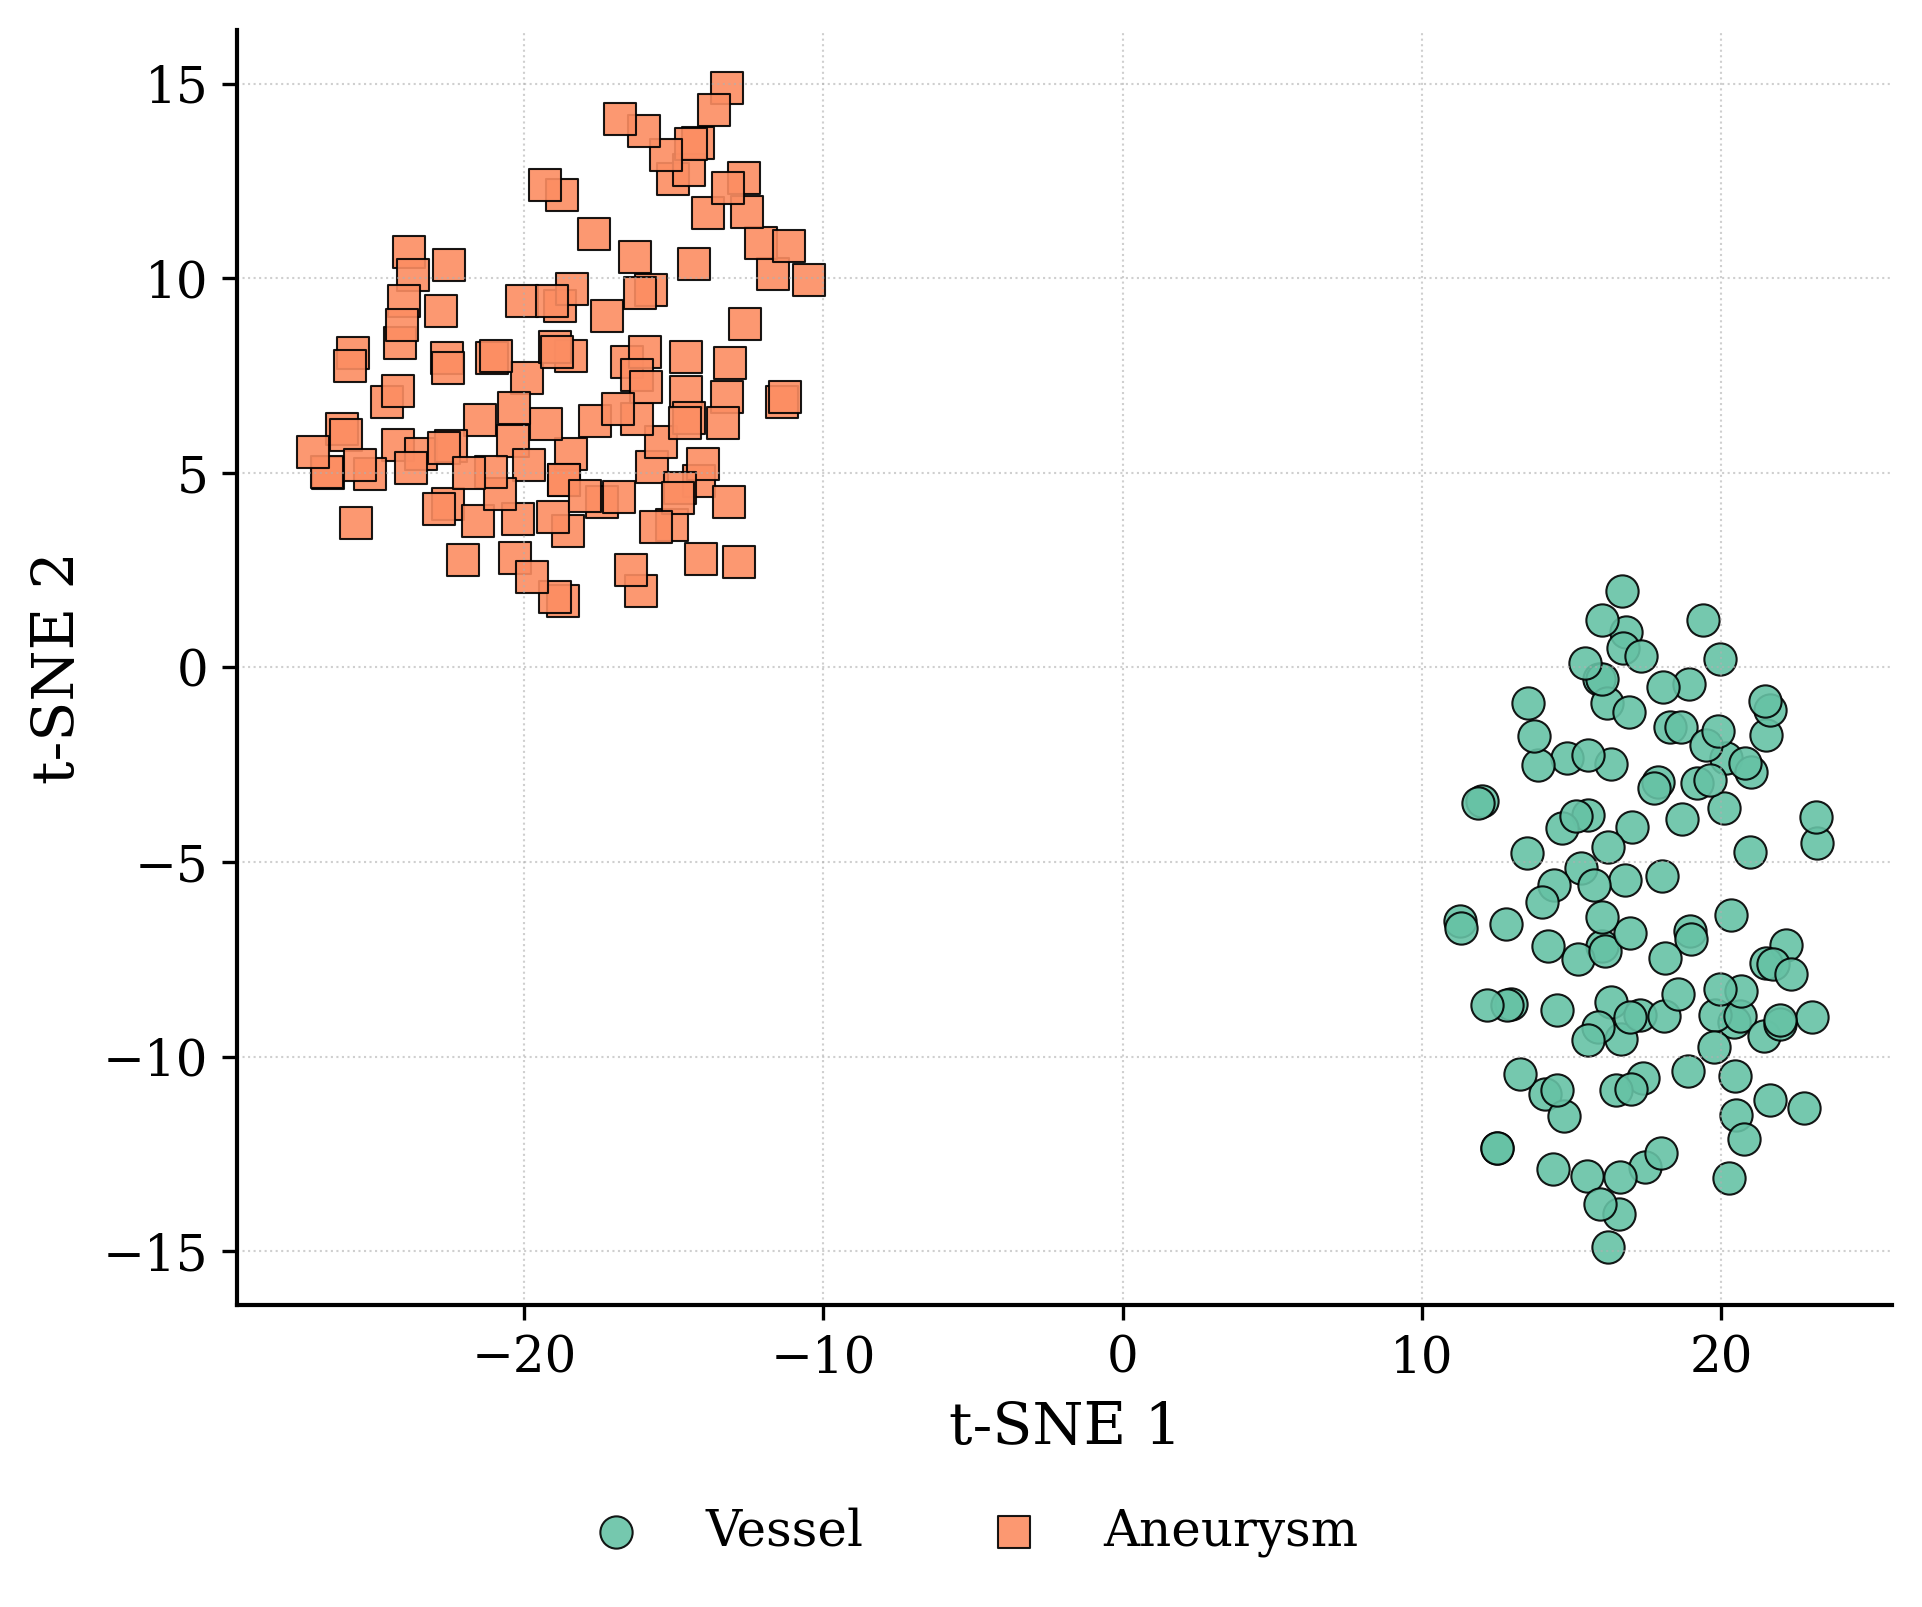
\includegraphics[width=0.34\textwidth]{t-sne_global_std.png}
  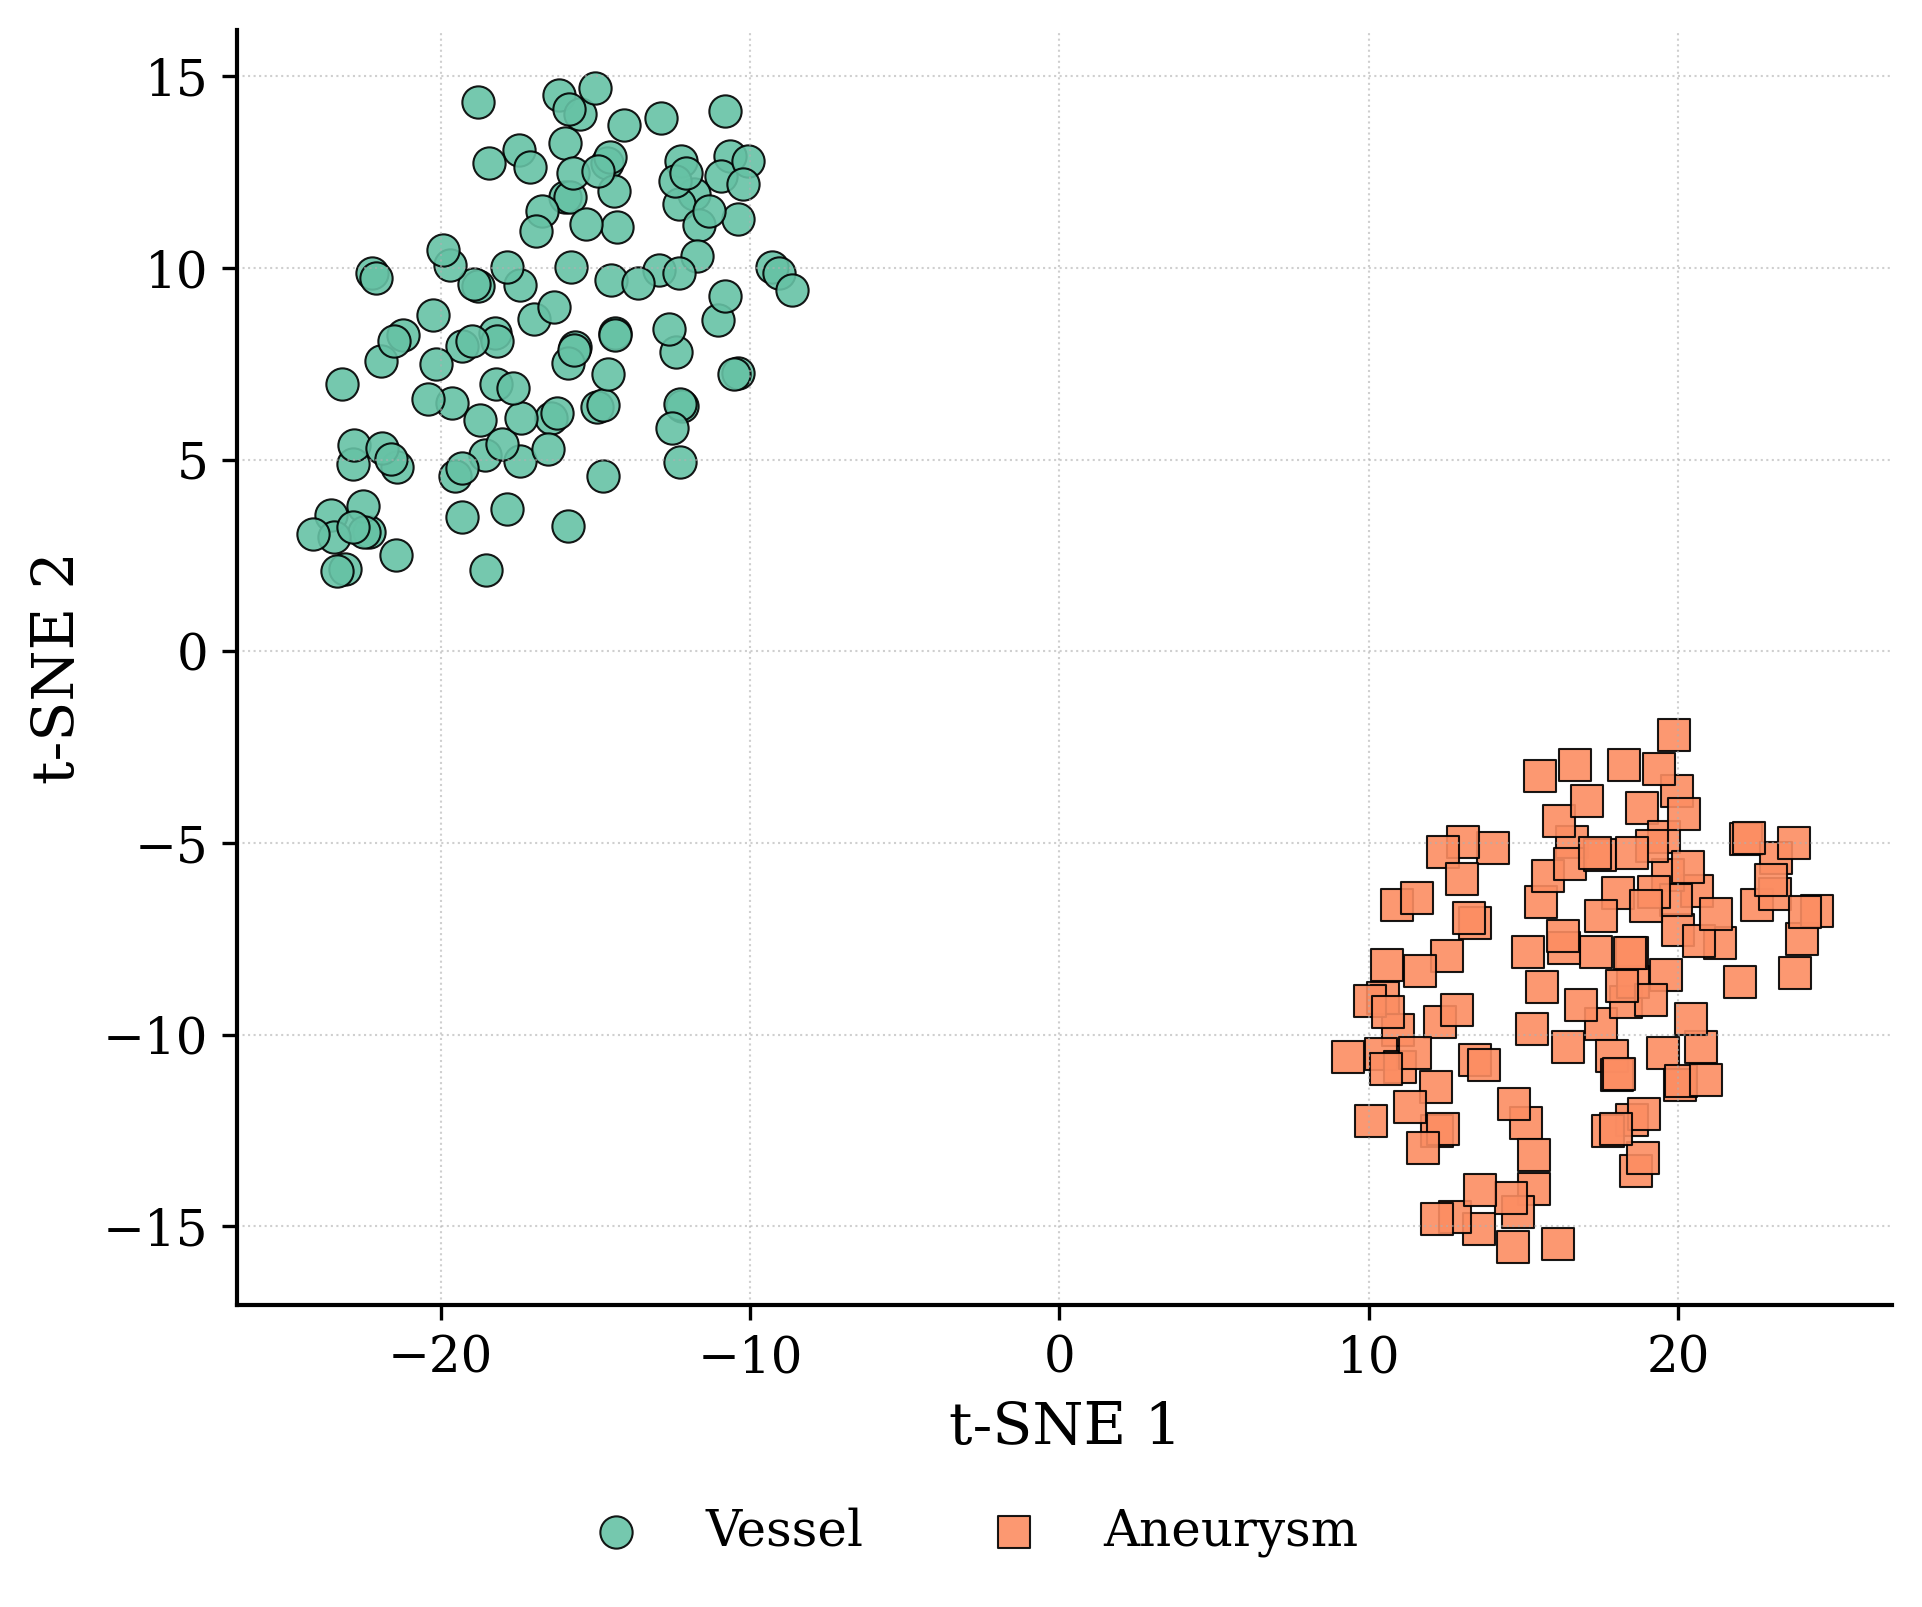
\includegraphics[width=0.34\textwidth]{t-sne_global_min.png}
  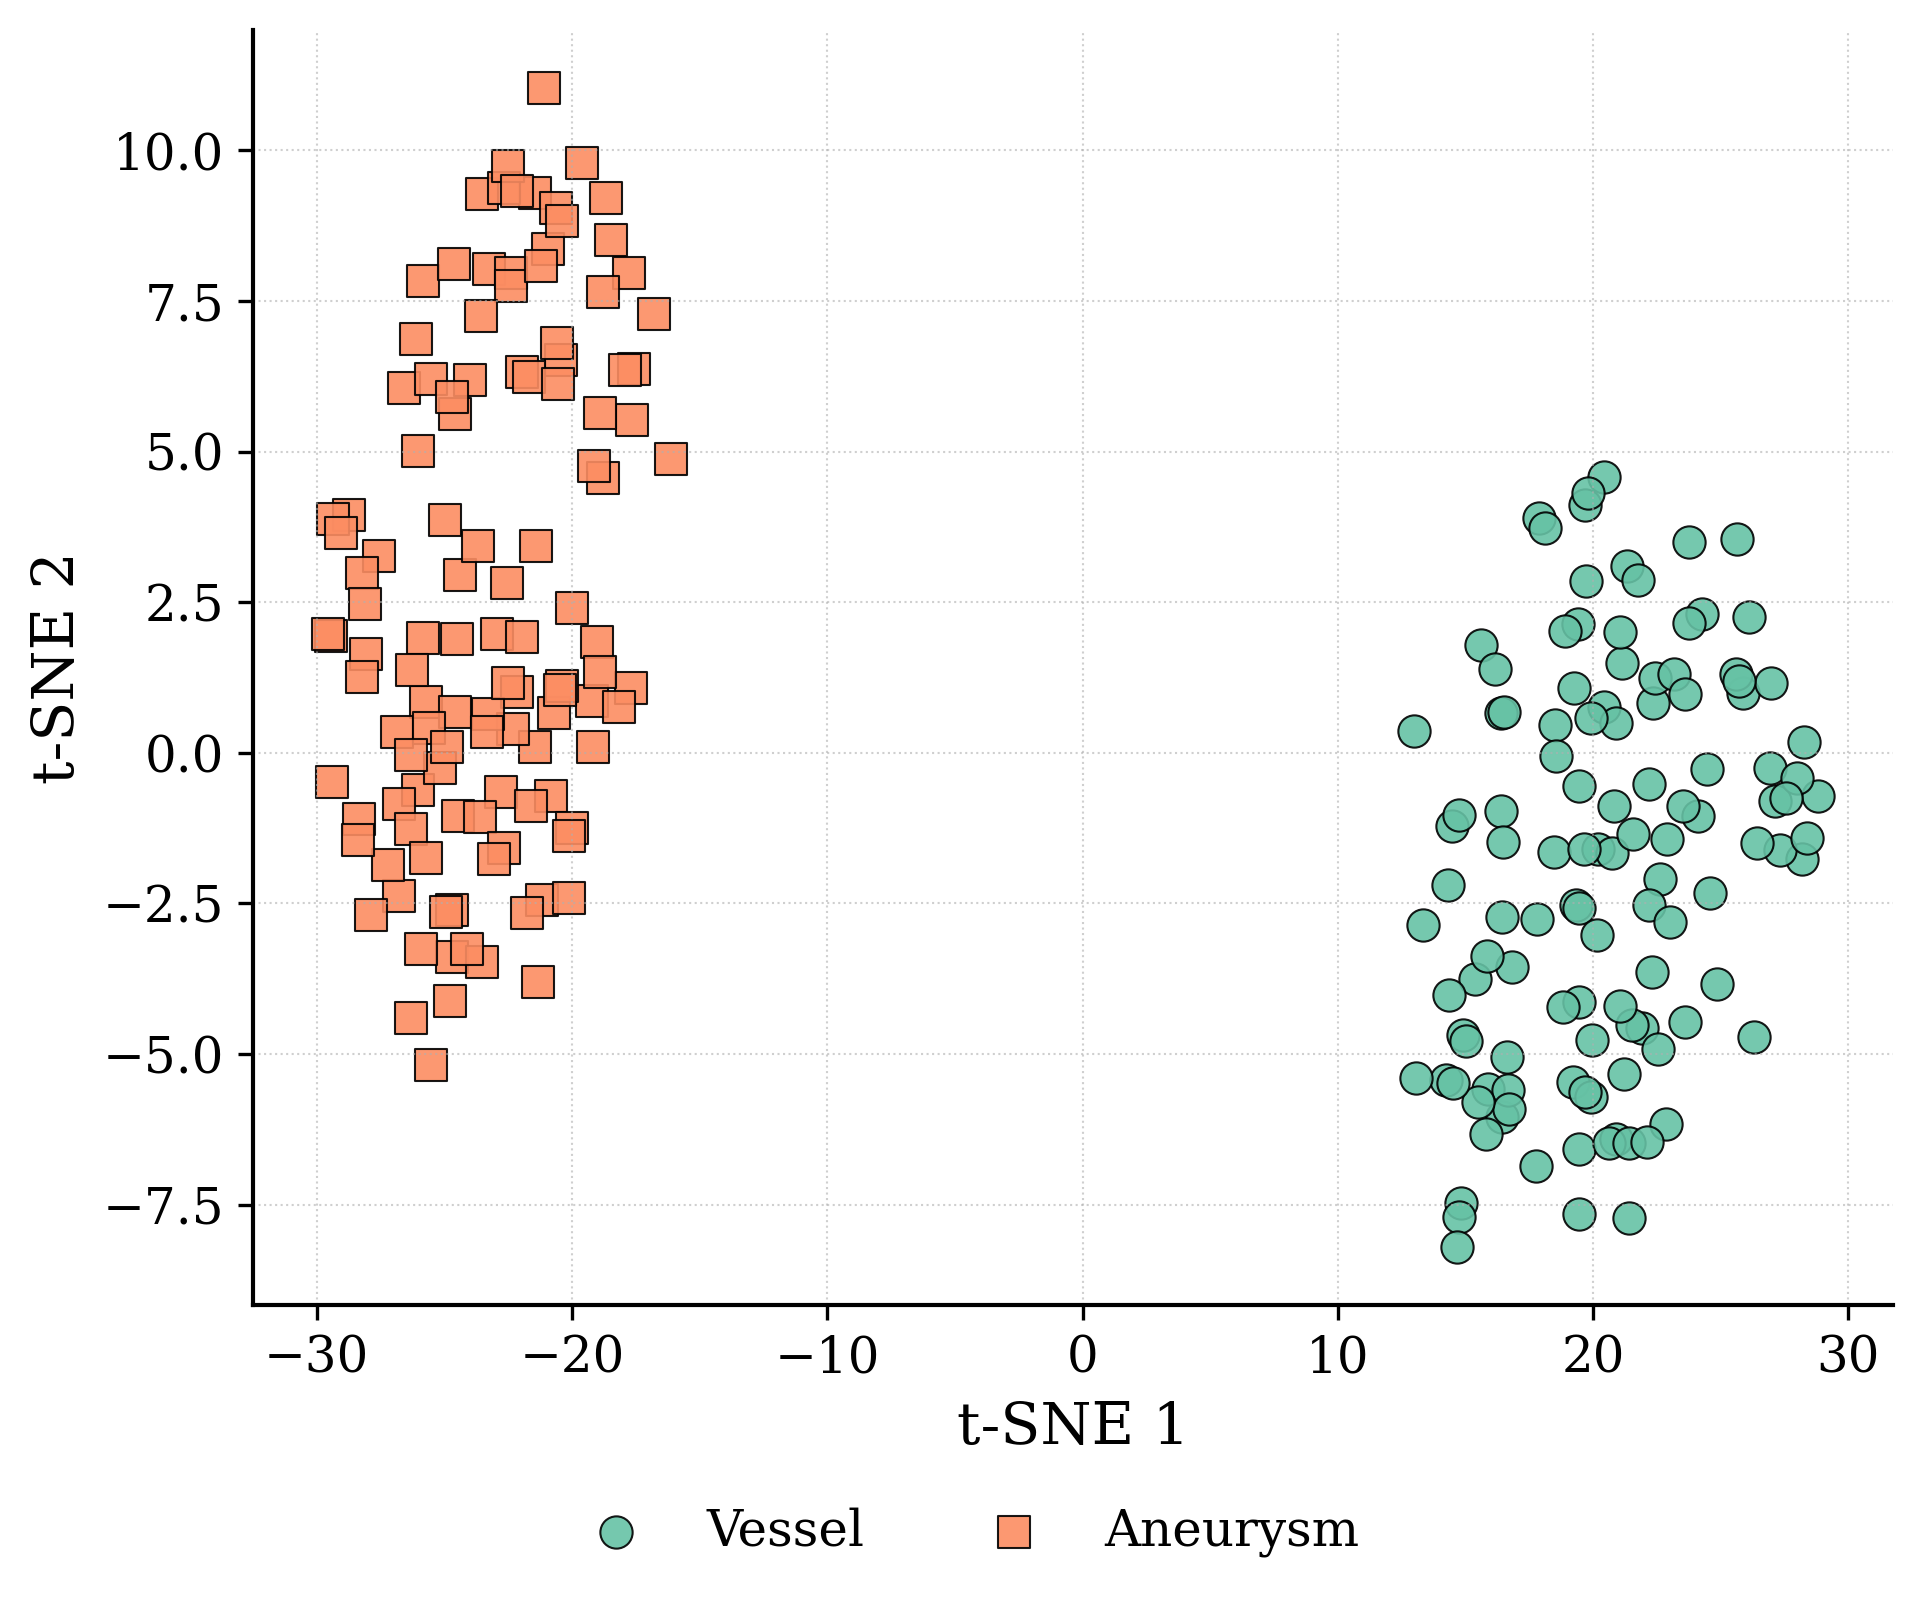
\includegraphics[width=0.34\textwidth]{t-sne_global_max.png}
  \caption{Results of t-SNE on annotated aneurysms over the Intra3D segmentation dataset. Figures show the mean, standard deviation, minimum, and maximum of the t-SNE components of the aneurysm and the vessel parts.}
  \label{fig:aneu_seg_supplementary_tsne}
\end{figure}

\begin{figure}[h!]
  \centering
\begin{center}
\begin{tabular}{ccc}
    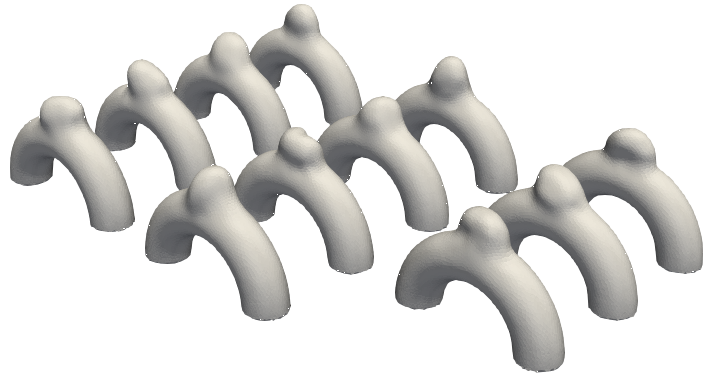
\includegraphics[width=0.330\textwidth]{cluster_2.png} &
    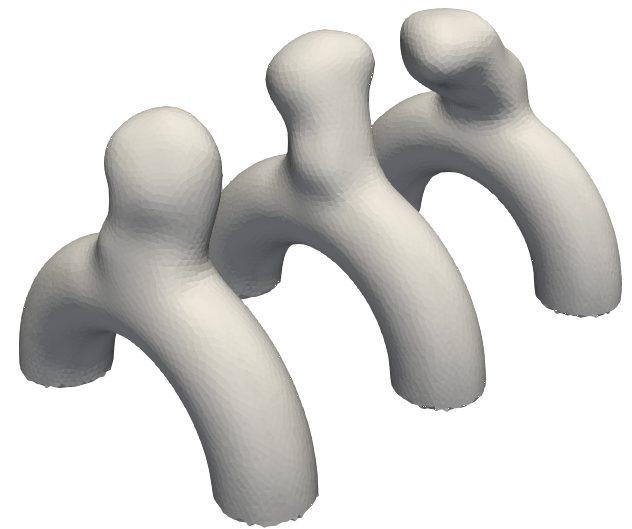
\includegraphics[width=0.200\textwidth]{cluster_6.png} &
    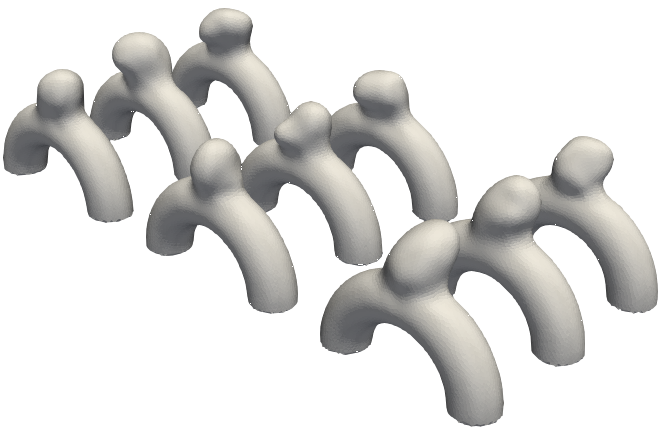
\includegraphics[width=0.300\textwidth]{cluster_0.png} \\
    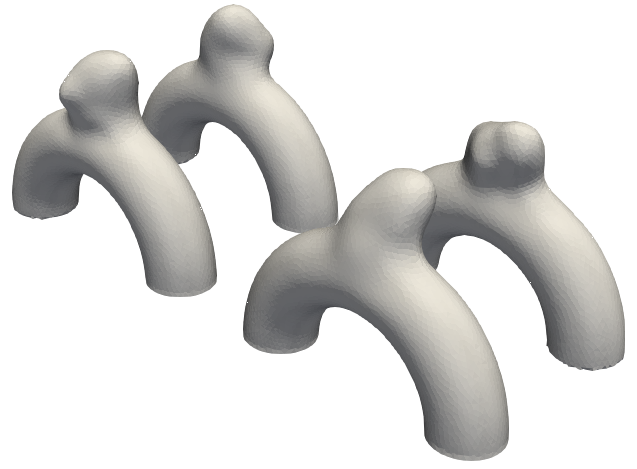
\includegraphics[width=0.249\textwidth]{cluster_3.png} &
    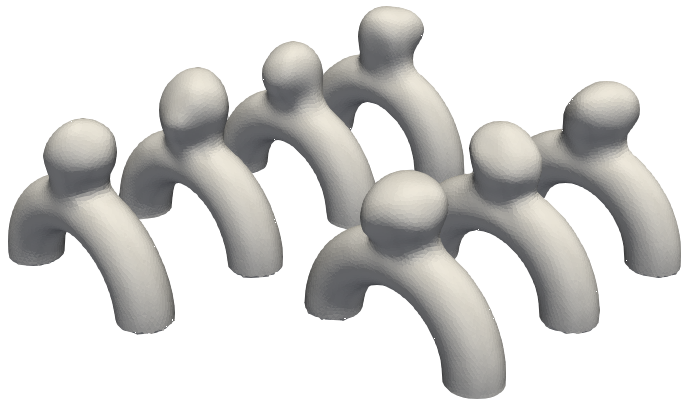
\includegraphics[width=0.319\textwidth]{cluster_4.png} &
    \includegraphics[width=0.289\textwidth]{cluster_5.png} \\
    \includegraphics[width=0.330\textwidth]{cluster_1.png} &
    \includegraphics[width=0.269\textwidth]{cluster_7.png} &
    \includegraphics[width=0.319\textwidth]{cluster_8.png} \\
    \includegraphics[width=0.310\textwidth]{cluster_9.png} &
    \includegraphics[width=0.310\textwidth]{cluster_10.png} &
    \includegraphics[width=0.205\textwidth]{cluster_11.png} \\
    \includegraphics[width=0.314\textwidth]{cluster_12.png} &
    \includegraphics[width=0.283\textwidth]{cluster_13.png} &
    \includegraphics[width=0.314\textwidth]{cluster_14.png} \\
\end{tabular}
\end{center}
\caption{Clusters of aneurysms from the AnXplore dataset \citep{anxplore} based on the t-SNE from mean features of the aneurysms.}
  \label{fig:clustering_supplementary}
\end{figure}



\end{document}